% Options for packages loaded elsewhere
\PassOptionsToPackage{hyphens}{url}
%
\documentclass[12pt, openany]{book}
\usepackage[top=2.2cm, left=2.2cm, bottom=1.6cm, right=1.8cm]{geometry} % Custom margins

\usepackage{pdfpages}
\usepackage{appendix}

\usepackage{listings}
\usepackage{xcolor}

\usepackage{float}
\usepackage{array}  % for better column formatting

\usepackage{cite} % for IEEE citation format

% Adding titlesec package
\usepackage{titlesec}
\usepackage{tabularx} % for better table control

% Redefining the chapter title format
\titleformat{\chapter}[display]
{\normalfont\huge\bfseries}{\chaptertitlename\ \thechapter}{20pt}{\Huge}
\titlespacing*{\chapter}{0pt}{-50pt}{10pt}

% Define colors for syntax highlighting
\definecolor{commentcolor}{gray}{0.5}
\definecolor{keywordcolor}{rgb}{0,0,1}
\definecolor{stringcolor}{rgb}{0.58,0,0.82}

\lstset{
	language=C++,  % Set the language
	basicstyle=\ttfamily\fontsize{10pt}{12pt}\selectfont,  % Set font style and size to 10pt with a normal line spacing of 12pt
	breaklines=true,  % Automatic line breaking
	captionpos=b,  % Caption at the bottom
	numbers=left,  % Line numbers on the left
	numberstyle=\tiny\color{gray},  % Styling for the line numbers
	numbersep=5pt,  % Space between line numbers and code
	xleftmargin=5pt,  % Margin on the left outside the frame
	frame=none,  % No frame around the code
	showstringspaces=false,  % Don't show spaces in strings with special character
	tabsize=4,  % Size of tabs
	commentstyle=\color{commentcolor}\ttfamily,
	keywordstyle=\color{keywordcolor}\bfseries\ttfamily,  % Bold for keywords
	stringstyle=\color{stringcolor}\ttfamily,
	morecomment=[l][\color{magenta}]{\#}
}

\renewcommand{\bibname}{References}

\usepackage{fontspec}
\setmainfont{Carlito}

\usepackage{amssymb,amsmath}
\usepackage{ifxetex,ifluatex}
\ifnum 0\ifxetex 1\fi\ifluatex 1\fi=0 % if pdftex
  \usepackage[T1]{fontenc}
  \usepackage[utf8]{inputenc}
  \usepackage{textcomp} % provide euro and other symbols
\else % if luatex or xetex
  \usepackage{unicode-math}
  \defaultfontfeatures{Scale=MatchLowercase}
  \defaultfontfeatures[\rmfamily]{Ligatures=TeX,Scale=1}
  \usepackage{fontspec}
  \setmainfont{Carlito}
\fi
% Use upquote if available, for straight quotes in verbatim environments
\IfFileExists{upquote.sty}{\usepackage{upquote}}{}
\IfFileExists{microtype.sty}{% use microtype if available
  \usepackage[]{microtype}
  \UseMicrotypeSet[protrusion]{basicmath} % disable protrusion for tt fonts
}{}

\makeatletter
\@ifundefined{KOMAClassName}{% if non-KOMA class
	\IfFileExists{parskip.sty}{%
		\usepackage{parskip}
	}{% else
		\setlength{\parindent}{0pt}
		\setlength{\parskip}{6pt plus 2pt minus 1pt}}
}{% if KOMA class
	\KOMAoptions{parskip=half}}
\makeatother
\usepackage{xcolor}
\IfFileExists{xurl.sty}{\usepackage{xurl}}{} % add URL line breaks if available
\IfFileExists{bookmark.sty}{\usepackage{bookmark}}{\usepackage{hyperref}}
\hypersetup{
	hidelinks,
	pdfcreator={LaTeX via pandoc}}
\urlstyle{same} % disable monospaced font for URLs
\usepackage{longtable,booktabs}

% Correct order of tables after \paragraph or \subparagraph
\usepackage{etoolbox}
\makeatletter
\patchcmd\longtable{\par}{\if@noskipsec\mbox{}\fi\par}{}{}
\makeatother
% Allow footnotes in longtable head/foot
\IfFileExists{footnotehyper.sty}{\usepackage{footnotehyper}}{\usepackage{footnote}}
\makesavenoteenv{longtable}
\usepackage{graphicx}
\makeatletter
\def\maxwidth{\ifdim\Gin@nat@width>\linewidth\linewidth\else\Gin@nat@width\fi}
\def\maxheight{\ifdim\Gin@nat@height>\textheight\textheight\else\Gin@nat@height\fi}
\makeatother
% Scale images if necessary, so that they will not overflow the page
% margins by default, and it is still possible to overwrite the defaults
% using explicit options in \includegraphics[width, height, ...]{}
\setkeys{Gin}{width=\maxwidth,height=\maxheight,keepaspectratio}
% Set default figure placement to htbp
\makeatletter
\def\fps@figure{htbp}
\makeatother
\setlength{\emergencystretch}{3em} % prevent overfull lines
\providecommand{\tightlist}{%
  \setlength{\itemsep}{0pt}\setlength{\parskip}{0pt}}

% Include fancyhdr for header and footer customization
\usepackage{fancyhdr}

% Page style setup
\pagestyle{fancy}
\fancyhf{} % clear all header and footer fields
\fancyfoot[C]{\thepage} % put the page number in the center of the footer
\renewcommand{\headrulewidth}{0pt} % no line in header area
\renewcommand{\footrulewidth}{0pt} % no line in footer area

% Ensure the plain page style, used on chapter opening pages, is also empty
\fancypagestyle{plain}{
	\fancyhf{} % clear all header and footer fields for plain pages
	\fancyfoot[C]{\thepage} % page number in the center of the footer on plain pages
	\renewcommand{\headrulewidth}{0pt}
	\renewcommand{\footrulewidth}{0pt}
}



\usepackage{titlesec}

% Formatting the chapter title to remove "Chapter X"
\titleformat{\chapter}[display]
{\normalfont\huge\bfseries}{}{0pt}{\Huge}


\begin{document}
\begin{titlepage}
	\centering
	% Title
	\vspace*{1cm} % Adjust the vertical space as needed
	{\Huge\bfseries Individual Project\\[0.5cm] Final Report\par}
	\vspace{2cm}
	% Reset centering to left-align the rest
	\raggedright
	% ID Number
	ID Number: B820928\par
	
	% Programme
	Programme: Electronic and Electrical Engineering MEng\par
	
	% Module Code
	Module Code: 23WSD030/23WS50META\par
	
	% Project Title
	Project Title: Thread by Thread: Benchmarking and Comparing the Executions of Multi-threaded Applications on Multi-core Architectures.\par
	
	% Abstract Heading
	\textbf{Abstract:}\par % Making 'Abstract' bold
	% Abstract Text
	% Background, aims, methods, results/conclusions.

	Modern processors, both in desktop and embedded systems, increasingly feature multi-core architectures. This project aimed to optimise three applications using parallel computing techniques to decrease runtime and enhance scalability, testing them on desktop and embedded processors, including the Raspberry Pi 5. The applications included \texttt{mpbenchmark}, a benchmarking tool for multi-core performance; \texttt{MobileNet}, a machine learning application for image classification originally single-threaded and adapted to use the \texttt{OpenMP} library for multi-threading; and \texttt{DeBaTE-FI}, a GUI for testing microcontrollers for soft errors, optimised with Python’s multi-processing and a high-performance C++ library for telnet communication. Results showed significant performance improvements: \texttt{mpbenchmark} was redesigned with modern \texttt{C++} and SIMD intrinsics, improving scalability and design; \texttt{MobileNet} achieved an 87\% performance increase on desktop processors, with a 60-65\% gain on Raspberry Pi; and \texttt{Debate-FI} saw a 43.5-62.1\% reduction in runtime across various setups. The project's contributions include a novel \texttt{C++} benchmark tool, a parallel version of the \texttt{MobileNet} CNN model, and an optimised \texttt{Debate-FI} platform, all demonstrating enhanced performance and scalability.

\end{titlepage}


\newpage
\tableofcontents

\chapter{Introduction(3-5 pages)}
The objective of this project is to enhance the performance of specific applications through parallel computing and to examine their efficiency on both desktop and embedded central processing units (CPUs). Parallel computing is a methodology employed in software development that enables certain segments of code to execute simultaneously, thereby diminishing the overall execution time of an application and augmenting its scalability. Contemporary processors boast a multi-core architecture, integrating multiple CPUs within a single chip, which is pivotal for facilitating parallelism\cite{modern_processors}.  

Parallelism can be achieved via multi-threading and multi-processing techniques. A process refers to an active instance of a computer program, encompassing the program's code and its ongoing activities. Each process operates within its distinct memory address space and system resources, maintaining independence from other processes. However, processes can engage in communication with one another through various inter-process communication (IPC) mechanisms. Conversely, a thread represents the minimal unit of processing within a process. It executes within a process's context, sharing the process’s resources like memory and file descriptors, yet it retains its distinct execution state, including the program counter, register set, and stack. Threads can facilitate the parallel execution of code segments within a single process\cite{multi_processing_multi_threading_article}.

Multi-processing involves an application initiating multiple processes to perform parallel operations, whereas multi-threading pertains to an application that generates multiple threads usually within a single process. This project concentrates on three main applications: the initial two are optimised utilizing multi-threading and their outcomes are assessed on both desktop and embedded processors. The embedded processors examined in this study include the Raspberry Pi 5, 4, and 3, with the Raspberry Pi 5 representing the forefront of technology as of 2024. The final application is a graphical user interface (GUI) application, where multi-processing is employed to attain parallelism. This application was developed by Alex Henneman, a Ph.D. student, under the supervision of Dr. Luciano Ost\cite{debate_fi_publication}. The aim here is to refine this application to minimize its execution time and enhance its scalability. 

The first objective of this project is to improve the \texttt{mpbenchmark} multi-core benchmark tool, which simulates jet engine thermodynamics to evaluate CPU performance \cite{mpbenchmark_paper}. \texttt{mpbenchmark} generates two key outputs: runtime and the number of deadlines missed, the latter indicating performance quality based on thread completion times. This tool builds upon its predecessor, \texttt{JetBench}, which was originally developed in \texttt{C} using \texttt{OpenMP} \cite{JetBench_paper}. The transition to \texttt{mpbenchmark} addresses \texttt{JetBench}'s limitations and extends support to other languages like \texttt{Ada}, \texttt{C\#}, and \texttt{Java}, with \texttt{C} and \texttt{Ada} showing the best performance. However, these versions face challenges such as \texttt{C}'s lack of object-orientation and manual memory management issues \cite{c_language_drawbacks}, and \texttt{Ada}'s limited use outside defense and aerospace \cite{ada_langauge_uses}. To overcome these, the project aims to develop \texttt{mpbenchmark} using \texttt{C++}, leveraging modern enhancements to improve functionality and efficiency since 2011.

The secondary objective of this project centres on enhancing the performance of \texttt{MobileNet}, a specialised machine learning algorithm within the realm of convolutional neural networks (\texttt{CNNs})\cite{mobilenet_paper}. \texttt{MobileNet} excels in the field of image classification, a process in which the algorithm is provided with an image and tasked with determining the image's corresponding class. While the intricate mathematical foundations and specific operational details of \texttt{MobileNet} are beyond the scope of this discussion, the primary focus is set on augmenting its efficiency. Originally designed as a sequential algorithm, \texttt{MobileNet} primarily operates on a single CPU core, which poses limitations on its execution speed and scalability. In pursuit of addressing these constraints, this project endeavours to transform the existing \texttt{C++} implementation of \texttt{MobileNet}\cite{mobilenet_repo} into a multi-threaded architecture. By doing so, the aim is to significantly decrease its runtime and enhance its scalability, thereby optimizing the algorithm's performance for more robust and efficient image classification tasks. This effort to transition \texttt{MobileNet} from a sequential to a multi-threaded model represents a strategic move to leverage the capabilities of modern multi-core processors, ensuring a more responsive and efficient computational process.

The project's third objective is dedicated to the optimisation of a graphical user interface (\texttt{GUI}) application designed for microcontroller (\texttt{MCU}) testing, with a focus on minimising application runtime and bolstering its scalability. Named the \texttt{DeBaTE-FI} platform\cite{debate_fi_publication}, this application is crafted in \texttt{Python} and leverages both multi-threading and multi-processing techniques to achieve parallelism and concurrency. It's crucial to distinguish between concurrency and parallelism; in a concurrent framework, tasks are initiated, executed, and completed in overlapping intervals, without necessitating simultaneous operation. The operational flow of the \texttt{DeBaTE-FI} platform involves the user connecting \texttt{MCUs} to a computer, after which the application dispatches specific commands to these \texttt{MCUs}. Following the transmission of commands, the platform awaits responses from the \texttt{MCUs} and proceeds to log the requisite data into output files. Among the three applications addressed in this project, the \texttt{DeBaTE-FI} platform emerges as the most intricate, a complexity attributable to both the scale and the sophisticated nature of its functions. This optimisation effort aims to streamline these extensive operations, enhancing the application's performance and user experience.

The report is structured as follows: It begins with a literature review that contextualises the research within the field by examining relevant studies. This is followed by the methodology section, which details strategies for identifying and addressing performance bottlenecks in the software, illustrated through Unified Modelling Language (UML) diagrams and code snippets. The results and discussion sections then present and analyse the performance enhancements observed in experiments conducted on desktop and Raspberry Pi models 3 through 5, with benchmark runtime and speedup plots quantifying the improvements. The discussion evaluates the optimisations' effectiveness and suggests future research directions, linking practical outcomes with theoretical implications. Appendices follow the conclusion, providing supplementary materials such as experimental setup details, system specifications, and extended code snippets to enhance understanding and ensure the report's transparency and reproducibility.


\section{Original contributions of this project}

\begin{enumerate}
	\item A novel multi-core benchmark application has been developed using the latest \texttt{C++} features, this application built upon the previous \texttt{mpbenchmark}\cite{mpbenchmark_paper} application. It outperformed the previous \texttt{mpbenchmark} implementations in \texttt{C} and \texttt{Ada} by 11\%, 4\% and 1\% on desktop, Raspberry Pi 5 and 4 respectively in terms of run time and provided better speedup across threads. Moreover the novel benchmark application also utilised SIMD intrinsics which provided up to an astonishing 70\% reduction in run time, this unprecedented improvement provided means of analysing the target CPU's SIMD operations ability. A publication describing the contribution of this project has been submitted to SBCCI(Symposium on Integrated Circuits and System Design) conference part of IEEE(Institute of Electrical and Electronics Engineers) organisation. 
	
	\item The development of the first multi-threaded \texttt{MobileNet} CNN(convolutional neural network) model. This enhanced CNN model has been used as a case study to assess the behaviour of multi-threaded applications running on multi-core processors under neutron radiation. A publication describing this CNN model has been submitted to IEEE RADECS(``RADiation Effects on Components and Systems") conference.
	
	\item The optimised redesign of the \texttt{DeBaTE-FI} platform\cite{debate_fi_publication} resulted in up to 60\% reduction in run time. Moreover a high performance \texttt{C++} library was developed for \texttt{telnet} communication with microcontrollers. The enhanced \texttt{DeBaTE-FI} platform produced a 43.5\% reduction in run time when testing 36 \texttt{STM32F767ZI} microcontrollers when tested in PhD research office in Loughborough University(Figure ~\ref{fig:debate_fi_setup}).
\end{enumerate}


\chapter{Literature review(6-10 pages)}
\section{Introduction}
The research topic focuses on parallel computing to optimize algorithms for both desktop and embedded CPUs. Parallel computing is widely regarded as a complex area within engineering and computer science. To develop or enhance multi-threaded solutions, a thorough understanding of the underlying algorithms and the specific goals of the application is crucial. This foundational knowledge is essential before attempting any modifications to ensure that changes do not deviate from the application’s original objectives. In our project, we concentrate on three applications: \texttt{mpbenchmark}, \texttt{MobileNet}, and \texttt{DeBaTE-FI} platform. It is imperative to understand the background and functionality of these applications by utilising the existing publications centred around them. 

Another goal of the literature review is to identify existing solutions to avoid duplicating efforts. Adherence to programming best practices is also a critical aspect of the project, given the complexity of parallel computing. This project strives to ensure that all developed software solutions conform to the best practices and guidelines recommended by industry experts, necessitating a comprehensive literature review.

The literature review is structured to support the report's overall organization, with individual subsections dedicated to the three main objectives, the review covers providing background information, reviewing current research, and offering critical analysis. The review then explores build systems, focusing on how this project aims to develop cross-platform applications that can operate on different operating systems such as \texttt{Linux}, \texttt{Windows}, or \texttt{macOS}. Further research is directed towards software design and multi-threading in line with modern \texttt{C++} guidelines, including discussions on relevant libraries, tools, and research on parallel algorithms. The conclusion section summarizes the findings from the preceding sections and underscores the significance of the reviewed literature to the research question.

\section{Objective 1: \texttt{mpbenchmark}}
% Brief overview and relevance to the project 
% Discussion of methodologies used in the studies.
% Summary of major findings related to the theme.
% Critical evaluation of the strengths, weaknesses, and gaps.

Our initial focus is on the original \texttt{JetBench} software, which was featured in a publication arising from an international conference held annually in Germany. This conference, part of the ARCS (Architecture of Computing Systems) series, boasts a tradition spanning over 30 years and is renowned for presenting cutting-edge research in computer architecture and operating systems. The specific conference relevant to the first objective of this project took place in 2010. Following the conference, a book was published containing a compilation of papers presented at the event. Our project specifically examines the paper titled ``JetBench: An Open Source Real-Time Multiprocessor Benchmark", authored by Muhammad Yasir Qadri, Dorian Matichard, and Klaus D. McDonald-Maier. This paper is of particular interest to our research as it introduces a multiprocessor benchmark software that aligns well with our project's goals, providing a foundational tool for assessing real-time multiprocessor performance\cite{JetBench_paper}.

The \texttt{JetBench} software emerged in response to the observed scarcity of real-time, multi-threaded benchmarks. Designed to simulate the thermodynamic calculations of jet engines in real time, \texttt{JetBench} serves as an application benchmark that not only simulates a realistic workload but also measures the time required to complete these calculations with different thread counts. Its primary objective is to assess the multi-core capabilities of CPUs. The workload generated by \texttt{JetBench} predominantly consists of Arithmetic Logic Unit (ALU) centric operations, including integer and double precision multiplication, addition, and division. These operations facilitate the computation of critical mathematical functions such as exponentiation, square roots, and conversions including the calculation of pi and degree-to-radian conversions. The software exhibits a significant parallel portion, constituting 88.6\% of its total operations. \texttt{JetBench} is developed in the \texttt{C} programming language and utilizes the \texttt{OpenMP} library to enable multi-threading, ensuring both efficiency and scalability. Furthermore, \texttt{JetBench} prioritizes portability, allowing it to assess the performance of a wide spectrum of systems, from low-end to high-end. This design philosophy ensures the avoidance of system-specific libraries or timers, underlining the software’s broad applicability and utility in performance evaluation across diverse computing environments.

The first paper\cite{JetBench_paper} provides valuable insights into the foundational aspects of this application benchmark, though it is not without its limitations. For instance, the application encompasses a limited scope of computations, a decision made to ensure compatibility with lower-end CPUs. However, this constraint may render the application seemingly inadequate for testing on more advanced CPUs. Additionally, the omission of input/output operations was a deliberate choice to enhance the application's portability, albeit at the expense of being unable to assess the I/O capabilities of the target platform. Despite these limitations, the benchmark's strength lies in its portability and its efficacy in evaluating the multi-core performance across a spectrum of computing systems, from low to high-end. These attributes deem the application an apt selection for this project, which seeks to explore and develop multi-threading capabilities for both desktop and embedded platforms.

To address the identified limitations of the \texttt{JetBench} software, a novel solution was devised using diverse programming languages. This innovation was detailed in a publication titled ``Using JetBench to Evaluate the Efficiency of Multiprocessor Support for Parallel Processing,'' authored by HaiTao Mei and Andy Wellings. The paper, released in 2014, was part of the proceedings of a notable conference\cite{mpbenchmark_paper}.

In their research, the authors of \texttt{mpbenchmark}\cite{mpbenchmark_paper} adopted an object-oriented programming (OOP) approach for C\# and Java implementations. They standardized result collection by executing the application 30 times with a varying number of threads, employing a specific Linux command to control CPU core usage. Results were collected using a desktop CPU and \texttt{Simics}(a virtual platform to simulate a high end 128-core CPU).  This methodology is in line with standard practices for benchmark data collection.

The authors of \texttt{mpbenchmark}\cite{mpbenchmark_paper} highlighted several design flaws in the original \texttt{JetBench} software\cite{JetBench_paper}, including the excessive use of shared variables leading to inaccurate performance results, race conditions from variables shared across threads, and erroneous benchmark output data printing. To remedy these issues, they restructured the \texttt{JetBench} code and introduced implementations in \texttt{Ada}, \texttt{C\#}, and \texttt{Java}. Notably, the compiled languages (\texttt{C} and \texttt{Ada}) demonstrated superior performance. Additionally, the impact of virtual cores enabled by simultaneous multi-threading (SMT) was observed to vary inconsistently across different programming languages.

In the second paper\cite{mpbenchmark_paper} several limitations were found. Firstly, the data collection, based on just 30 runs, may be insufficient, especially for applications with minimal execution times on high-end CPUs. Additionally, the research focused solely on desktop CPUs and a system simulator mimicking a high-end 128-core CPU, excluding experiments on embedded or lower-end CPUs. Furthermore, given the superior performance of compiled languages like C and Ada, further research could beneficially explore comparisons with \texttt{C++}, another compiled language often regarded as superior to both C and Ada in certain contexts. This paper lays a solid foundation for our project, where its limitations present opportunities for further investigation, and its methodological approaches offer a model for emulation.

\section{Objective 2: \texttt{MobileNet}}
% Brief overview and relevance to the project 
% Discussion of methodologies used in the studies.
% Summary of major findings related to the theme.
% Critical evaluation of the strengths, weaknesses, and gaps.

\texttt{MobileNet} is a specialized machine learning algorithm that falls under the category of convolutional neural networks (CNNs). Developed specifically for mobile and embedded vision applications, \texttt{MobileNet} is discussed in detail in a 2017 paper by Cornell University titled ``MobileNets: Efficient Convolutional Neural Networks for Mobile Vision Applications"\cite{mobilenet_paper}. 

This paper\cite{mobilenet_paper} delves into the mathematical foundations required to construct the \texttt{MobileNet}, which are considered beyond the scope of our project. To summarize, the \texttt{MobileNet} architecture employs depth-wise separable convolutions that enhance memory efficiency and leverage optimized numerical linear algebra algorithms to reduce latency.

\texttt{MobileNet} introduces two crucial hyper-parameters: the width and resolution multiplier. These allow for adjustments to the model's size and computational requirements, with smaller \texttt{MobileNet} models typically showing slightly reduced accuracy compared to their larger counterparts. In comparative analyses with other renowned models like \texttt{GoogleNet}, \texttt{VGG 16}, and \texttt{FaceNet}; \texttt{MobileNet} offers comparable accuracy levels.

Despite its advantages of reduced size and latency, making it ideal for mobile and embedded devices, the paper\cite{mobilenet_paper} does not address the use of parallel computing techniques, presenting an opportunity for further exploration of its source code to enhance performance through parallelism.

For the practical component of our project, a \texttt{C++} implementation of \texttt{MobileNet} was chosen, sourced from a public repository on the \texttt{GitHub}\cite{mobilenet_repo}. This particular implementation was part of a computer science competition\cite{mobilenet_competition}, challenging participants to classify images into 20 predefined classes using provided training, validation, and testing data, with submissions made in a \texttt{.zip} file format.

The \texttt{C++} implementation comprises several header and source files but lacks build software or instructions, which poses a significant initial hurdle. Moreover, the implementation features a method for testing custom images against 12 predefined classes. However, these class names are in Chinese, necessitating translation into English for broader accessibility. Setting up and running the project before making any enhancements will be challenging. Nevertheless, this \texttt{C++} implementation presents a valuable opportunity to apply parallelisation techniques to improve the efficiency of the widely recognized \texttt{MobileNet} algorithm.

\section{Objective 3: \texttt{DeBaTE-FI platform}}
% Brief overview and relevance to the project 
% Discussion of methodologies used in the studies.
% Summary of major findings related to the theme.
% Critical evaluation of the strengths, weaknesses, and gaps.

The \texttt{DeBaTE-FI} platform, developed by PhD student Alex Henneman under the supervision of Dr. Luciano Ost at Loughborough University, is a GUI application detailed in the publication ``DeBaTE-FI: A Debugger-Based Fault Injector Infrastructure for IoT Soft Error Reliability Assessment." While not publicly available, this document can be accessed in appendix \ref{appendix:debate_fi}.

\texttt{DeBaTE-FI} was engineered to test embedded devices for soft errors—random errors in processors caused by background radiation, which can be particularly harmful in safety-critical systems. Testing methods for soft errors range from high-level analytical models, which are easier to implement but less accurate, to costly full radiation tests, which offer higher precision. \texttt{DeBaTE-FI} seeks to emulate the latter's accuracy by simulating soft errors in embedded devices. The platform utilized \texttt{Raspberry Pi 4} and \texttt{Rock 4C} to conduct tests on \texttt{STM32F7} microcontrollers (MCUs). The research involved running a neural network binary on these MCUs, measuring the execution time across various testing scenarios, and using different numbers of MCUs to evaluate speed and efficiency. Additionally, the results from \texttt{DeBaTE-FI} were compared with those from simulation software to assess accuracy, and \texttt{OpenOCD} was used for MCU communication.

The authors observed that increasing the number of MCUs reduced overall runtime. They also discovered that while multithreading in Python did not improve performance, multiprocessing—which enables parallel processing—did enhance performance significantly. The study confirmed that \texttt{DeBaTE-FI} provides greater accuracy than the high-level simulation software they aimed to surpass. Challenges arose when using \texttt{Raspberry Pi 4}, particularly with USB controller limitations that restricted the connection to no more than 8 MCUs, prompting a switch to \texttt{Rock 4C}, which supported up to 30 MCUs but also reached full CPU utilization under this load.

Despite the innovative approach of \texttt{DeBaTE-FI}, the platform is hindered by several significant limitations. The primary issue is its lengthy runtime, which can extend to several minutes, suggesting the presence of performance bottlenecks. Moreover, the performance on embedded Linux devices, such as \texttt{Rock 4C}, is modest, highlighting the need for optimization across both desktop and embedded Linux devices (or single-board computers). Additionally, the utilization of \texttt{OpenOCD} for MCU communication presents an opportunity to enhance efficiency and expedite processes. The central goal of our project is to tackle these issues by improving the runtime efficiency and scalability of \texttt{DeBaTE-FI}.

\section{Cross platform build systems}
When researching cross platform build systems this is an area of software engineering that is rapidly evolving therefore finding peer reviewed publications was a difficult task. Instead research was conducted using online blogs and relevant books. Since our project focuses on creating \texttt{C++} applications, there is a need to automate the building and compiling process. There exists many tools that allow for this to happen. Moreover the project also must ensure that the applications created work on multiple operating systems such Linux, Windows or macOS. This is important as Linux maybe the go to operating system for most developers, the majority of computers nowadays run Windows. Cross platform simply means that the application is able to run on multiple operating systems.  


\section{\texttt{C++} guidelines and best practices}

\section{Conclusion}
Summarize the main findings and debates covered in the review.
Reiterate the importance of the existing literature to your research question.
Outline how your research is positioned within the academic field based on your review.



\chapter{Methodology(5-7 pages)}
\section{Objective 1: \texttt{mpbenchmark}}
As mentioned in the introduction section \texttt{mpbenchmark} performs calculations of a jet engine using multiple threads and produces the time taken to complete these calculations as output. The source code of \texttt{mpbenchmark} provided a solution in \texttt{C\#}\cite{mpbenchmark_code}, this served as a useful reference of how would be implemented in code using object-oriented design. Subsequently, the \texttt{C++} object oriented design comprised of three main classes:

\begin{enumerate}
	\item \texttt{FileDataLoader}: the primary function of this class is to load data from the input file and also to allow the user to save output data to the output file.
	\item \texttt{SharedPerformanceData}: this class stores data loaded from the input file into an array and also allows storage of output data into a separate array. But importantly it allows threads to access specific parts of the input data in a thread-safe manner. 
	\item \texttt{Worker}: this class contains functions to perform the important calculations, computations of deadlines missed and output data. This class defines the \texttt{operator ()} which encapsulates the main calculations, this class design is know as a \texttt{Functor}.
\end{enumerate}

The \texttt{C++} object-oriented class design can be visualised using a UML class diagram shown in figure \ref{fig:mpbenchmark_UML_diagram}.

\begin{figure}[H] % Positioning preference: here, top, bottom, page
	\centering
	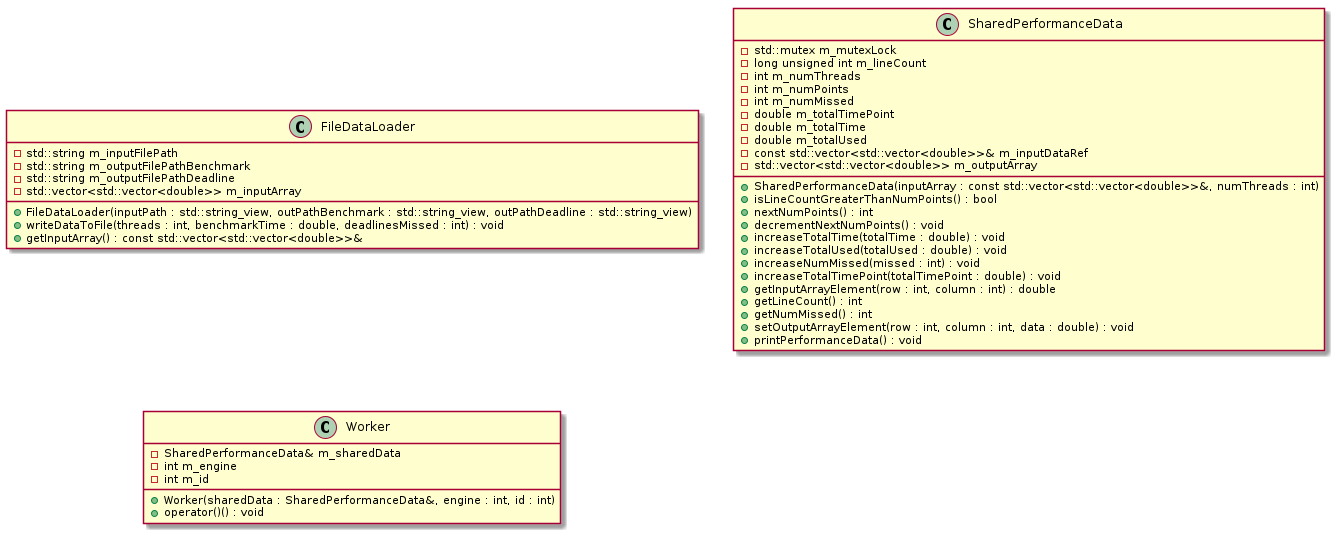
\includegraphics[width=1\textwidth, height=20cm]{~/Documents/Part_D_Modules/Individual_Project/Individual_report/figures/mpbenchmark_class.png} % Adjust the path and width as needed
	\caption{UML class diagram of the proposed \texttt{C++} solution.}
	\label{fig:mpbenchmark_UML_diagram} % Use this label to reference the figure
\end{figure}

Figure ~\ref{fig:mpbenchmark_UML_diagram2} shows the UML sequence diagram on how the three classes in the previous Figure ~\ref{fig:mpbenchmark_UML_diagram} are used. The ``\texttt{main}" in the sequence diagram represents the \texttt{.cpp} file where the \texttt{int main(...)} function exists. 

\begin{figure}[htbp] % Positioning preference: here, top, bottom, page
	\centering
	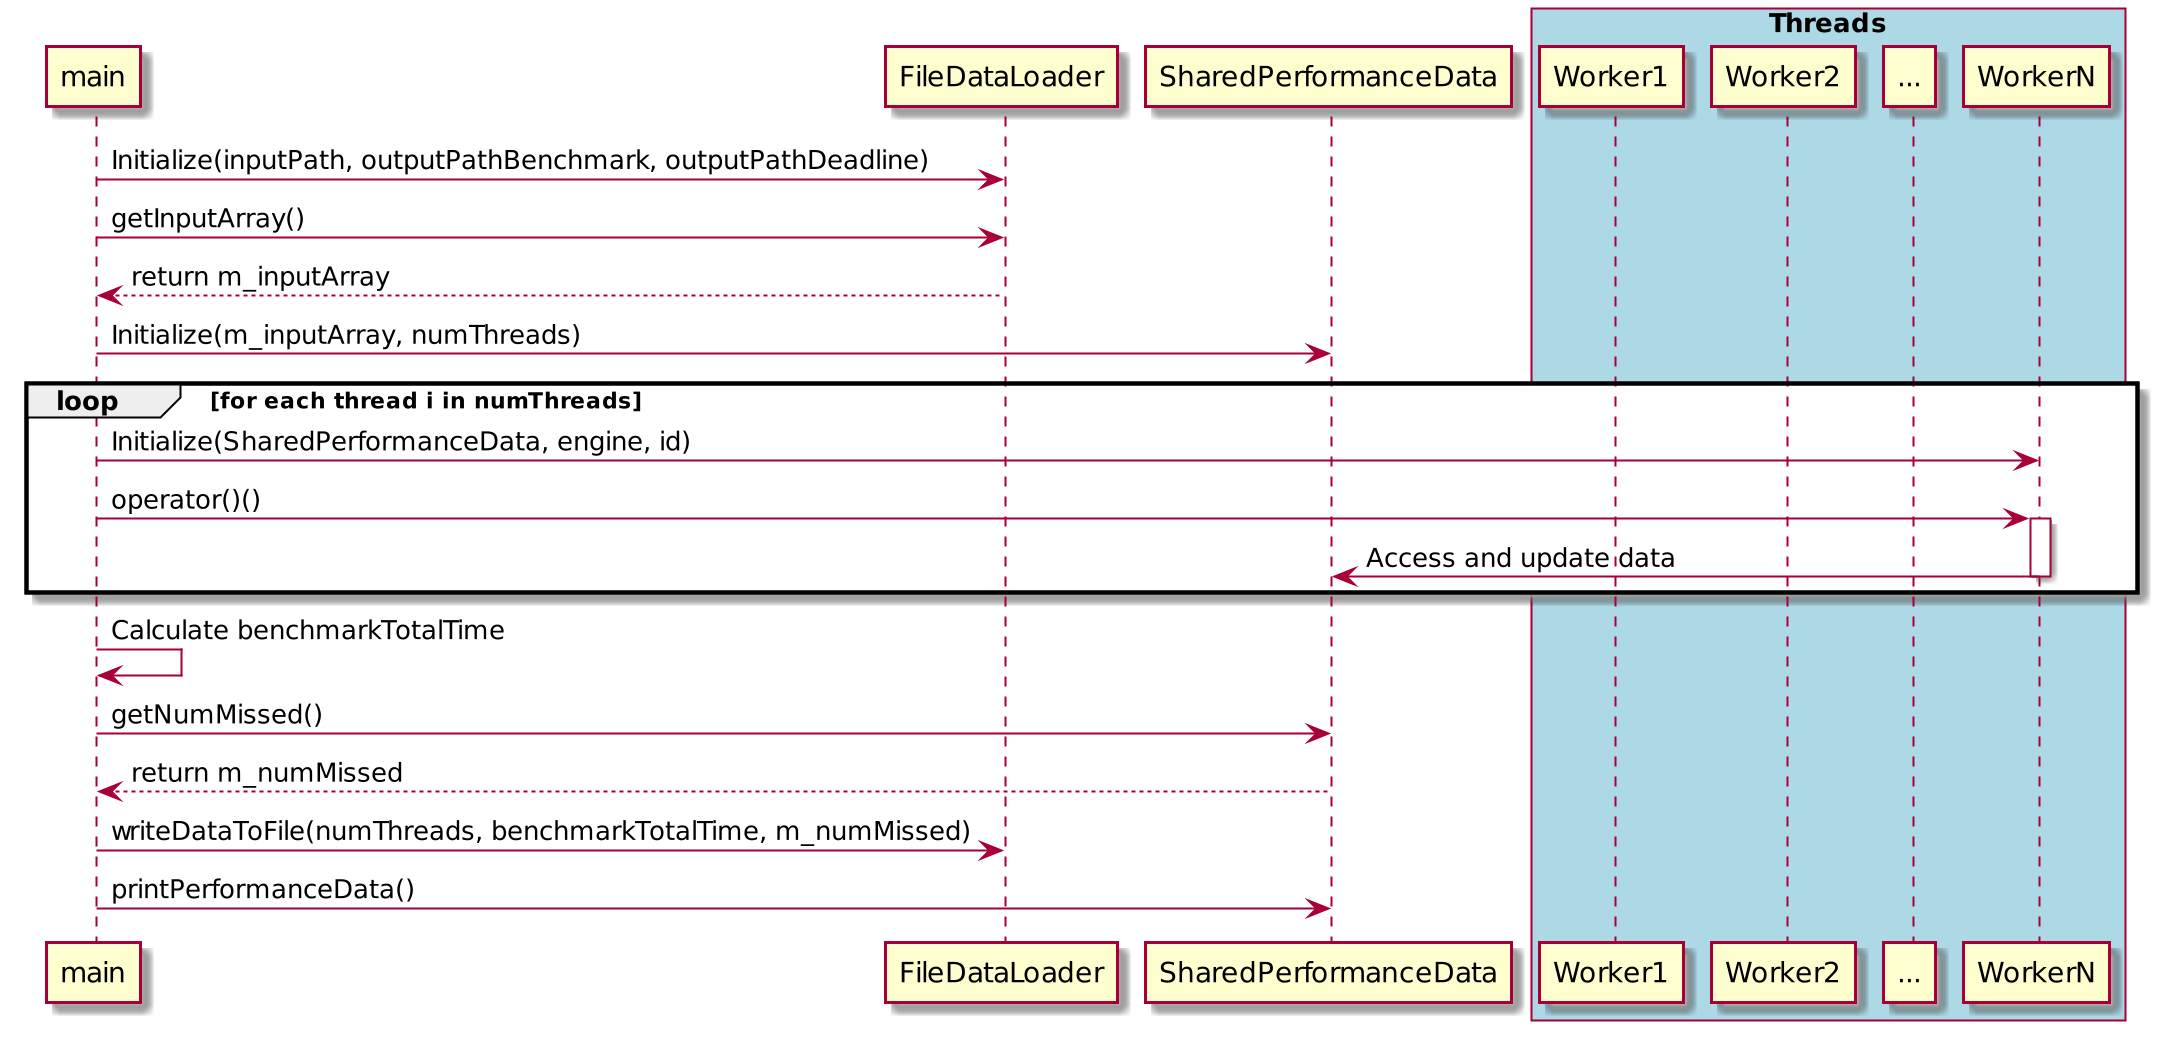
\includegraphics[width=1\textwidth, height=20cm]{figures/mpbenchmark_sequence.png} % Adjust the path and width as needed
	\caption{UML sequence diagram of the proposed \texttt{C++} solution.}
	\label{fig:mpbenchmark_UML_diagram2} % Use this label to reference the figure
\end{figure}

The key features of the proposed solution leverage the modern enhancements introduced to the \texttt{C++} language in its 2011 update. Since then, \texttt{C++} has undergone significant transformations that include advanced multi-threading capabilities and improved memory management techniques. Significantly, the introduction of \texttt{std::thread} and \texttt{std::mutex} in modern \texttt{C++} offers a more convenient and cross-platform approach to multi-threading compared to traditional \texttt{POSIX} threads, which are not only more cumbersome to use but also restricted to \texttt{Unix}-based systems. The utilization of these features in the proposed solution enhances its portability and ease of use. Additionally, the proposed solution incorporates the \texttt{std::vector} class, a dynamic array sequence container that significantly simplifies memory management. Unlike in the \texttt{C} language, where manual handling of dynamic memory can be error-prone, \texttt{std::vector} automates this aspect, thereby reducing complexity and potential bugs. While modern \texttt{C++} offers numerous advantages over \texttt{C}, including object-oriented programming features and performance parity, it does come with a steeper learning curve. This learning curve is often seen as a trade-off for the powerful features and robustness provided by \texttt{C++}\cite{evolution_of_C++}.

The proposed solution employed the \texttt{fmt} library in \texttt{C++}\cite{fmt_printing_library} for output, providing an enhanced printing method compared to the \texttt{std::cout()} function from the \texttt{C++} standard library. Although the compiler on the target system supported the \texttt{C++20} standard, it lacked support for the \texttt{std::format()} function, which provides better printing capabilities in \texttt{C++}\cite{std_format_gcc_compiler_version}. Additionally, a new command line argument was introduced to adjust the number of threads used, complementing the existing argument that modifies the simulation engine. For compilation and linking, the industry-standard \texttt{CMake}\cite{cmake_about} software was utilized. In the \texttt{CMakeLists.txt} file, essential configurations included specifying the \texttt{C++20} standard, incorporating the \texttt{fmt} library, and compiling with the \texttt{-O2} optimization flag. This optimisation flag, also used by the original authors of \texttt{mpbenchmark}\cite{mpbenchmark_paper}, was retained in the proposed solution for consistency.

An alternate solution was developed to further enhance the performance of \texttt{mpbenchmark}, the \texttt{Valgrind/Callgrind} function profiler tool was deployed to find potential bottlenecks. The application was compiled with debug information and optimisations turned off, this was done by specifying the build type as \texttt{Debug} and compiling with \texttt{-g} and \texttt{-O0} flags in the \texttt{CMake} file. \texttt{Callgrind} profiling shows ``self-cost" of different parts of the code. ``Self-cost" refers to the number of CPU cycles that were directly consumed by a specific function itself. This can be used to find potential areas of optimisations\cite{Valgrind2024}. \texttt{Callgrind} profiling results showed that part of the application where it approximates the value of $\pi$ had the highest self-cost. This code snippet is shown in the listing ~\ref{lst:pi_approximation_1} below:

\begin{lstlisting}[
	caption={Part of the code with the highest self-cost. It approximates $\pi$ using numerical integration.},
	label={lst:pi_approximation_1}
	]
// initialise variables for the pi calculation
const long num_steps = 1000000;
double step = 1.0 / static_cast<double>(num_steps);
double x{}, pi{}, sum{};

// performing numerical integration using the midpoint Riemann sum
for (int i = 0; i < num_steps; i++) {
	x = (i + 0.5) * step;
	sum += 4.0 / (1.0 + x * x);
}
pi = sum * step;
\end{lstlisting}

The problem with this part of the code was that it was already part of the parallel regions where it is executed by each thread. It may seen like a good candidate for applying parallel \texttt{for loop} from the OpenMP library however creating nested threads beyond the number of threads available on the system does not always lead to higher performance and in many cases can degrade performance. Another way to improve performance is by using SIMD intrinsics. An advantage of using \texttt{C++}(and/or \texttt{C}) is that SIMD intrinsics can be deployed whereas higher level languages like \texttt{Java} or \texttt{C\#} make it very difficult to access these. 

SIMD intrinsics vary by the target CPU, \texttt{x86} processors (which are found in most laptop and desktops) use \texttt{AVX2} instructions whereas \texttt{ARM} processors(commonly found in Apple products and embedded devices) use \texttt{NEON} instructions. In this project we use both as our proposed \texttt{C++} solution will be deployed on desktop(\texttt{x86} processor) and Raspberry Pi devices(\texttt{ARM} processor). The SIMD enhanced code can be summarised algorithmatically in the following steps in Figure ~\ref{fig:_simd_algorithm}.

\begin{figure}[htbp]
\centering
\begin{enumerate}
	\item Initialise \texttt{256-bit} wide vectors: each vector can hold four double-precision (\texttt{64-bit}) floating point numbers. The main initialisations would be a vector to hold four loop indices (\texttt{vec\_i}), a vector to calculate four values of $x$ (\texttt{vec\_x}), a vector to hold the result of the integrand (\texttt{vec\_temp}) and a vector to accumulate the sum (\texttt{vec\_sum}) after each loop iteration.
	\item \texttt{for loop} iterate until \texttt{num\_steps/4}:
	\begin{itemize}
		\item step 1: calculate the four midpoints $x$-values simultaneously using the vector \texttt{vec\_i} and hold result in \texttt{vec\_x}. Original formula used: \texttt{(i + 0.5) * step}.
		\item step 2: compute the value of the integrand in parallel using the four calculated $x$-values stored in \texttt{vec\_x}, store result in \texttt{vec\_temp}. Original formula used: \texttt{4 / (1 + x * x)}.
		\item step 3: accumulate the values from \texttt{vec\_temp} into the \texttt{vec\_sum} vector.
		\item step 4: increment loop indices vector \texttt{vec\_i} by \texttt{4}. 
	\end{itemize}
	\item Final summation: upon the completion of the loop, perform a horizontal sum on the vector (\texttt{vec\_sum}) that held the accumulated values.
	\item Calculation of $\pi$: sum is multiplied by the step size to approximate the value of $\pi$. Original formula used : \texttt{pi = sum * step}.
\end{enumerate}
\caption{Algorithm for calculating $\pi$ using SIMD(\texttt{AVX2}) instructions.}
\label{fig:_simd_algorithm}
\end{figure}


As discussed, to utilise SIMD intrinsics on Raspberry Pi devices, \texttt{NEON} instructions must be employed. \texttt{NEON} instructions come with limitations, notably in their support for double precision floating points, which is restricted, and their vector width, which is only \texttt{128-bit}, compared to the \texttt{256-bit} vectors seen in \texttt{AVX2}\cite{neon_reference}. To accommodate \texttt{NEON}, two solutions were developed: one using single precision floating points (\texttt{float}) and the other using double precision floating points (\texttt{double}). The \texttt{NEON} code with \texttt{float} can perform four computations simultaneously, while the code with \texttt{double} can manage only two computations simultaneously, due to the \texttt{128-bit} vector's capacity to store four \texttt{float} values or two \texttt{double} values. Typically, \texttt{float} variables offer less decimal precision than \texttt{double} variables. These two SIMD-enhanced solutions, along with their decimal accuracy levels, will be compared in the results and discussion section. The \texttt{NEON} implementation follows a similar algorithm as the one shown in Figure ~\ref{fig:_simd_algorithm}. The \texttt{CMake} file also required some changes to allow the \texttt{AVX2} instructions to be used, this along with the code snippets for the SIMD enhanced code can be found in the [Appendix \ref{sec:app_obj1}]. 

To collect benchmark data, the runtime was recorded and saved to a specified \texttt{.txt} file, the number of deadlines missed were also saved but in a separate \texttt{.txt} file. The application underwent 103 runs, with the first three designated as warm-up runs; the subsequent 100 runs were averaged and utilised for plotting bar charts and speedup plots. For the languages \texttt{Java} and \texttt{C\#}, data were collected over 103 runs. In contrast, for the compiled languages \texttt{C}, \texttt{Ada}, and \texttt{C++}, the application was executed 203 times. The variance in the number of threads was controlled using the \texttt{taskset} command in Linux. Specifically for the \texttt{C++} application, a second command line argument was employed to specify the number of threads. This approach aligns with the methodology described by the authors of \texttt{mpbenchmark}\cite{mpbenchmark_paper}. An example bash script demonstrating how the application was executed multiple times is shown in the following Listing ~\ref{lst:benchmark_collection}:

\begin{lstlisting}[
	caption={Bash script to run application multiple times along with \texttt{taskset} command. Command line arguments: \texttt{mpbenchmark [engine\_type] [threads]} .},
	label={lst:benchmark_collection}
	]
# Loop to run the executable 103 times, using "3" as the default engine type and 2 cores/threads 
for i in {1..103}
do
	taskset -c 0,2 ./mpbenchmark 3 2 
done

# Loop to run the executable 103 times, using "3" as the default engine type and 4 cores/threads 
for i in {1..103}
do
	taskset -c 0,2,4,6 ./mpbenchmark 3 4 
done
\end{lstlisting}

The process of collecting benchmark times can be visualised in the image shown in figure ~\ref{fig:results_collection}. The python application used to plot the graphs was trivial and not shared in this report. The full system specification of the desktop and Raspberry Pi devices used to collect data can be found in the [Appendix ~\ref{tab:spec_comparisons}]. The results are displayed via benchmark and speedup plots. A benchmark plot shows the mean run time of the application on the vertical axis with the number of cores or threads on the horizontal axis, in this case the lower is better as a lower run time indicates better performance. A speedup plot shows the speedup ratio on the vertical axis and the number of cores or threads on the horizontal axis, here higher values are better because a higher speedup indicates better scalability of the application. The ``speedup" is a ratio of the time taken for the application using a certain number of threads compared to the original single-threaded run time. For example, if an application takes 100 ms to run using 1 thread and 20 ms to run using 8 threads. The speedup for 8 threads would be $\frac{100}{20}$ equalling \texttt{5.00}, as a ratio it would be unitless. 

In summary, for desktop (\texttt{x86}) processors, two main solutions have been developed: a novel \texttt{C++} solution and a SIMD-enhanced \texttt{C++} solution as discussed in Listing~\ref{lst:pi_approximation_2}. For the Raspberry Pi devices, three solutions have been created: the first is the novel \texttt{C++} solution, identical to that on the desktop, and the other two are the SIMD-enhanced versions utilizing \texttt{NEON} instructions with single and double precision floating point variables.

\begin{figure}[htbp] % Positioning preference: here, top, bottom, page
	\centering
	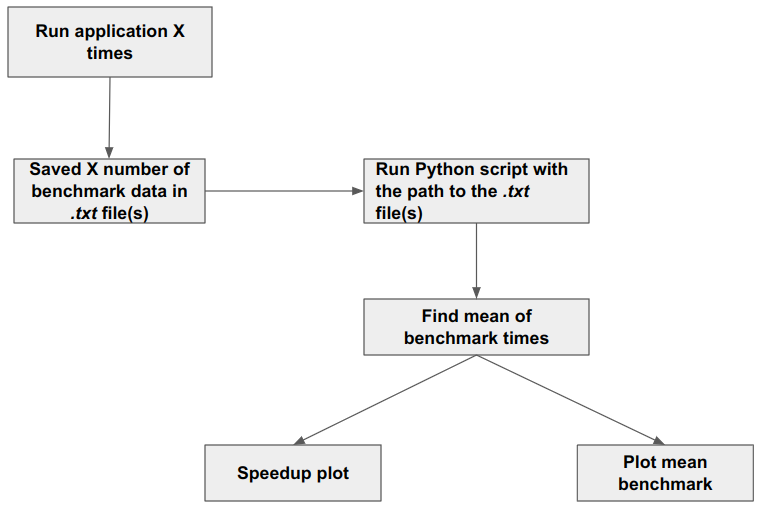
\includegraphics[width=0.5\textwidth]{~/Documents/Part_D_Modules/Individual_Project/Individual_report/figures/benchmarking_method.png} % Adjust the path and width as needed
	\caption{Benchmark results collection strategy.}
	\label{fig:results_collection} % Use this label to reference the figure
\end{figure}

\section{Objective 2: \texttt{MobileNet}}
% Step 1: MobileNet setup
% Step 2: Valgrind results
% Step 3: OpenMP parallelisations and SIMD
% Step 4: Raspberry Pi different compilations

Setting up MobileNet from the \texttt{GitHub} repository\cite{mobilenet_repo} was a time consuming task. Details about the setting up process can be found in the [Appendix Listing ~\ref{lst:mobilenet_updates}]. Once setup the \texttt{MobileNet} project needed to be profiled with \texttt{Callgrind} function profiler to find bottlenecks and possible parallelisation points. To use \texttt{Callgrind}, the project was compiled with debug information and no optimisations. This required setting the build type as \texttt{Debug} and adding \texttt{-g} and \texttt{-O0} optimisation flags in the \texttt{CMakeLists.txt} file. \texttt{Callgrind} results showed that functions from the convolution and batch normalisation layer had the highest self-cost. The functions with the highest self-cost were \texttt{ConvLayer::forward()}, \texttt{BatchNormalLayer::forward()} and \texttt{ConvLayer::Addpad()}. The detailed \texttt{Calgrind} profiling results can be seen in [Appendix Figure ~\ref{fig:mobilenet_profiling}]. 

The CPU intensive function inside the convolution layer contained a number of nested \texttt{for} loops with large iterations. \texttt{OpenMP} library was used to parallelise the \texttt{for} loops. The \texttt{collapse} clause and dynamical scheduling type of the parallel \texttt{for} loop from the \texttt{OpenMP} library were implemented inside the \texttt{ConvLayer::forward()} function. In the OpenMP library, the \texttt{parallel for} directive, enhanced by the \texttt{collapse(3)} clause and \texttt{dynamic} scheduling, efficiently manages the execution of nested loops in parallel. By collapsing three nested loops into a single sequence, the \texttt{collapse} clause simplifies load balancing across multiple threads by increasing the pool of iterations available for distribution. Concurrently, the \texttt{dynamic} scheduling type assigns iterations to threads in real-time, adapting to varying execution times among iterations and ensuring an even workload distribution\cite{openmp_guide}. 

To parallelise the other two functions \texttt{BatchNormalLayer::forward()} and \texttt{ConvLayer::Addpad()} only the \texttt{collapse} clause was utilised. The \texttt{ConvLayer::forward()} function contained some computations which were a good candidate for SIMD optimisations, these were more straight forward than compared to objective 1 as \texttt{OpenMP} library allows a simple way of using SIMD without the developer having to worry about \texttt{AVX2} or \texttt{NEON} instructions. For the Raspberry Pi processor it was decided to parallelise only the \texttt{ConvLayer::forward()}, \texttt{BatchNormalLayer::forward()} functions and not use the SIMD enhancements, as SIMD instruction's performance gains are more limited on embedded processors due to the narrower registers\cite{embedded_processors_reduced_simd_performance}. Having said that results from parallelising all the three functions and SIMD enhanced code were compared to find the optimal solution. This is discussed in the results and discussion section. 

To address the different compilations, the \texttt{CMake} file was altered. A macro \texttt{EMBEDDED\_PROC} was added. To compile the \texttt{MobileNet} project for \texttt{x86} processors the macro \texttt{EMBEDDED\_PROC} was set to \texttt{OFF}, this applies parallelisation to all three functions along with the SIMD enhancements. To compile the \texttt{MobileNet} project for Raspberry Pi processor the user can specify the \texttt{EMBEDDED\_PROC} to \texttt{ON}, this would parallelise only the two functions discussed and not apply SIMD enhancements. This can be seen in lines 15-18 in listing ~\ref{lst:mobilenet_parallel}. The parallelisation of the other two functions \texttt{BatchNormalLayer::forward()} and \texttt{ConvLayer::Addpad()} was very similar to \texttt{ConvLayer::forward} and can be found in [Appendix Listing ~\ref{lst:mobilenet_function1_parallel} and ~\ref{lst:mobilenet_function2_parallel}]. 

\begin{lstlisting}[
	caption={Parallelising the \texttt{ConvLayer::forward()} function and applying SIMD depending on the macro \texttt{EMBEDDED\_PROC}.},
	label={lst:mobilenet_parallel}
	]
void ConvLayer::forward(float *pfInput)
{
// collapse 3 "for" loops and use dynamic scheduling 
#pragma omp parallel for collapse(3) schedule(dynamic)
for (int g = 0; g < m_nGroup; g++)
{
	for (int nOutmapIndex = 0; nOutmapIndex < m_nOutputGroupNum; nOutmapIndex++)
	{
		for (int i = 0; i < m_nOutputWidth; i++)
		{
			
// other code to be ignored ... 
			
// Only use OpenMP SIMD optimizations if EMBEDDED_PROC is not defined 
			#ifndef EMBEDDED_PROC
			#pragma omp simd reduction(+:fSum)
			#endif
			for (int n = 0; n < m_nKernelWidth; n++)
			{
				nKernelIndex = nKernelStart + m * m_nKernelWidth + n;
				nInputIndex = nInputIndexStart + m * m_nInputPadWidth + n;
				fSum += m_pfInputPad[nInputIndex] * m_pfWeight[nKernelIndex];
			}
		}
	}              
}

}
\end{lstlisting}

In line 16 of the code snippet above(listing ~\ref{lst:mobilenet_parallel}) the reduction clause on the \texttt{fSum}, this ensured that after vectorized operations, the partial results held in different elements of the SIMD vector register are correctly summed up into the single scalar \texttt{fSum}. This avoids any manual management of these partial results, simplifying the code and ensuring correctness.

Moreover the arrays must also be aligned to make full use of the SIMD clause, this is important in several key ways. First, it ensures efficient utilisation of the CPU's cache lines, reducing cache misses by aligning data accesses with the processor’s cache system, thereby accelerating data retrieval. Second, it facilitates efficient SIMD operations, as modern SIMD instructions require data to be aligned with the size of their registers—here, 256 bits or 32 bytes—to prevent penalties from misalignment, such as additional cycles for data realignment. Alignment also prevents faults that occur when data is accessed at addresses not aligned to the required boundaries, particularly on systems where such misalignment leads to crashes. Lastly, by aligning memory accesses with the hardware's memory interface, the code optimises the throughput and maximizes the memory bandwidth usage. Together, these factors ensure that the SIMD-optimised processes in the convolutional layer computations are performed with maximal efficiency and stability. A 32-byte alignment was used for arrays \texttt{m\_pfInputPad} and  \texttt{m\_pfWeight}, this is shown in Listing  ~\ref{lst:mobilenet_array_alignment}.

\begin{lstlisting}[
	caption={Making arrays that are 32-byte aligned for SIMD clause.},
	label={lst:mobilenet_array_alignment}
	]
ConvLayer::ConvLayer(/*Constructor arguments not shown ... */) 
{
// ignore other code ... 

// Creating arrays which are 32-byte aligned for SIMD optimisations 
size_t alignment = 32;
size_t inputPadSize = m_nInputNum * m_nInputPadWidth * m_nInputPadWidth * sizeof(float);
size_t weightSize   = m_nOutputNum * m_nInputGroupNum * m_nKernelSize * sizeof(float);
size_t outputSize   = m_nOutputNum * m_nOutputSize * sizeof(float);

m_pfInputPad = static_cast<float*>(aligned_alloc(alignment, inputPadSize));
m_pfWeight   = static_cast<float*>(aligned_alloc(alignment, weightSize));
}
\end{lstlisting}

The \texttt{MobileNet} application was designed with three command line arguments. The first argument determines whether to classify only one image or all images in the \texttt{data} folder. The second argument specifies whether the runtime should be saved to a \texttt{.txt} file, and the third sets the number of threads used. For data collection, the time taken to classify a single image was recorded while varying the number of threads. The number of threads utilized by the application was adjusted using the command line and \texttt{OpenMP}'s \texttt{omp\_set\_num\_threads()} function. Additionally, \texttt{MobileNet} includes an option to save the application's runtime to a designated \texttt{.txt} file. For benchmarking, the project was compiled with the \texttt{-O3} optimisation flag and was executed 103 times with different thread counts; the runtime and speedup plots were derived from the average of the 100 timing results stored in the \texttt{.txt} file. The method of data collection largely mirrors the process shown in figure~\ref{fig:results_collection}, with the exception that the \texttt{taskset} command was not employed to adjust the number of CPU cores; instead, thread adjustments were made through the command line. The detailed code snippet of the command line arguments can be found in the [Appendix Listing ~\ref{lst:mobilenet_command_line_arguments}].  

\section{Objective 3: \texttt{DeBaTE-FI} platform}
% Talk about profiling the application 
% C++ libraries for telnetpp and integration into the Debate-FI via Pybind-11
% Multi-processing and mutli-threaidng design improvement 

The application was profiled to find bottlenecks and possible points of optimisations. The tool \texttt{py-spy} was used to profile the application and save the output as a \texttt{.json} file\cite{py-spy}. The results were then viewed using the \texttt{speedscope} web application\cite{speedscope_app}. Since the application used multi-processing, the required processes were identified and their process \texttt{pid} was used to run \texttt{py-spy}, as shown below in Listing~\ref{lst:py_spy_application}:

\begin{lstlisting}[
	caption={Running \texttt{py-spy} on the specified process.},
	label={lst:py_spy_application}
	]
	py-spy record --pid <PID> --format speedscope -o profile.json 
\end{lstlisting}


Profiling results showed that the functions from \texttt{Python}'s \texttt{Telnetlib} library had the highest self-cost. To optimize the application, a \texttt{C++} open-source \texttt{Telnet} library was utilized. The \texttt{C++} library, called \texttt{telnetpp},\cite{telnetpp_library} along with \texttt{serverpp},\cite{serverpp_library} was integrated into the application using the tool \texttt{pybind11}. \texttt{pybind11} is a lightweight library for integrating \texttt{C++} into \texttt{Python} applications\cite{pybind11}. The \texttt{telnetpp} library required some functions for it to be integrated into the application; thus, a wrapper class in \texttt{C++} was created that allowed \texttt{telnetpp} to seamlessly replace the previous \texttt{telnetlib} \texttt{Python} library. The wrapper \texttt{C++} class was named \texttt{telnetlibcpp} for consistency. This \texttt{C++} class is shown in the following UML class diagram (Figure~\ref{fig:telnetlibcpp_UML}). The main functions used, \texttt{Readout()}, \texttt{Exec()}, and \texttt{write()}, have the exact same names as the functions from the \texttt{Python} library. Profiling results and detailed code snippet about the \texttt{C++} functions can be found in [Appendix ~\ref{sec:app_obj3}]. 

\begin{figure}[htbp] % Positioning preference: here, top, bottom, page
	\centering
	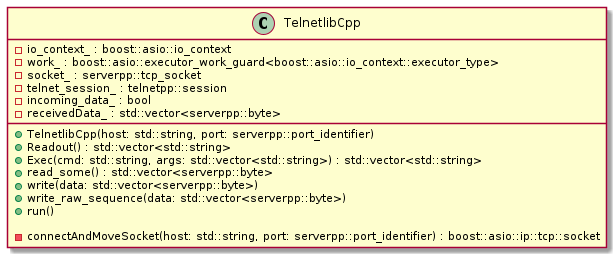
\includegraphics[width=1\textwidth, height=15cm]{~/Documents/Part_D_Modules/Individual_Project/Individual_report/figures/telnetlib_C++_class.png} % Adjust the path and width as needed
	\caption{\texttt{C++} class to emulate \texttt{Python's} \texttt{telnetlib} library functions.}
	\label{fig:telnetlibcpp_UML} % Use this label to reference the figure
\end{figure}

Using \texttt{CMake} and \texttt{pybind11} the \texttt{C++} class was compiled into a shared library(\texttt{.so}) file which was then moved into the same directory as the application. This allowed the \texttt{python} application to call the \texttt{C++} functions and use the \texttt{telnetpp} \texttt{C++} library. 

Another solution was developed which aimed to optimise the application's multi-processing and multi-threading. A simplified version of the application's architecture is shown below in the UML sequence diagram(Figure ~\ref{fig:original_application_arch}):

\begin{figure}[htbp] % Positioning preference: here, top, bottom, page
	\centering
	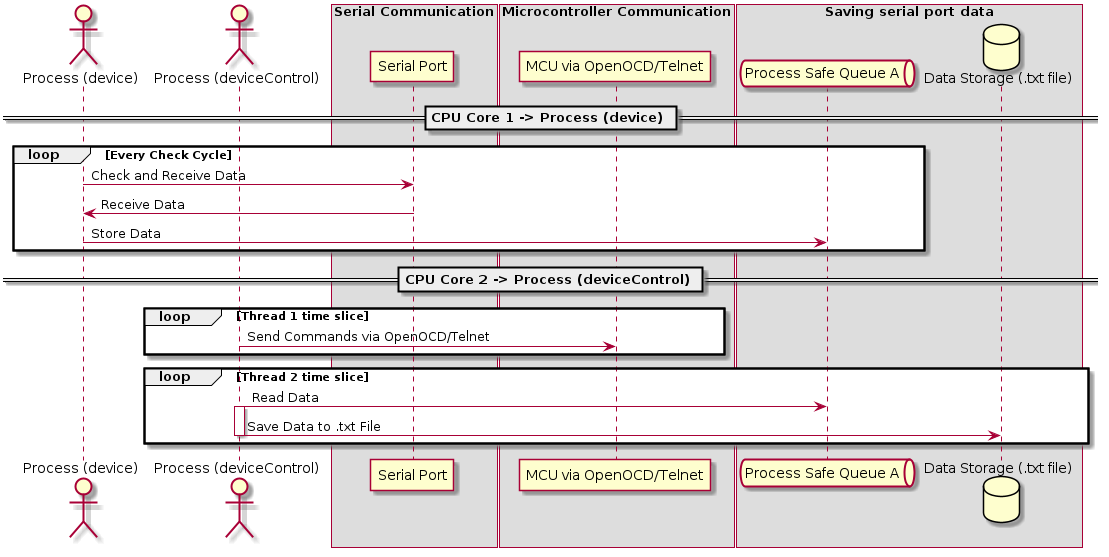
\includegraphics[width=1\textwidth, height=15cm]{~/Documents/Part_D_Modules/Individual_Project/Individual_report/figures/original_process_design.png} % Adjust the path and width as needed
	\caption{The sequence of the original application architecture. CPU Core 2 has to split CPU time between handling serial port data and sending commands.}
	\label{fig:original_application_arch} % Use this label to reference the figure
\end{figure}

Figure ~\ref{fig:original_application_arch} summarises how the original application had a convoluted design leading to poor performance:

\begin{enumerate}
	\item Two classes \texttt{device} and \texttt{deviceControl} spawned processes. 
	\item The \texttt{deviceControl} process had its workload split between sending commands to MCU and saving serial port data to \texttt{.txt} file.  
	\item The \texttt{device} process seem to be performing a redundant task of saving serial port data into a queue. 
\end{enumerate}

This design was improved as follows:

\begin{enumerate}
	\item Two classes \texttt{device} and \texttt{deviceControl} spawn processes with each having their own designated tasks.
	\item The \texttt{deviceControl} process now only sends data to the MCU.   
	\item The \texttt{device} process only focuses on receiving data from the serial port and saving it to the \texttt{.txt} file. 
\end{enumerate}

The key in the above improved design is removing the redundant work done as previously both of the processes were handling the serial port data. Handling serial port data does not require two processes it can be done using only one. When threads are used inside a process CPU time is split between the two threads. In the improved design both processes only perform one task and more importantly the \texttt{deviceControl} process has a reduced workload, this is important as the CPU time will be fully allocated to sending commands to the MCU . The challenge here was to make sure both of the processes were synchronised. This was accomplished using the \texttt{Event()} object from the \texttt{multiprocessing} \texttt{Python} library. When the \texttt{deviceControl} process started it sent a signal to the \texttt{device} process, to start checking and storing serial port data, and when the \texttt{deviceControl} process finished it sent a signal to stop the \texttt{device} process, stopping the \texttt{device} process would then save the accumulated serial port data into the \texttt{.txt} file. This can be visualised in the following UML sequence diagram (Figure ~\ref{fig:improved_application_design}):

\begin{figure}[htbp] % Positioning preference: here, top, bottom, page
	\centering
	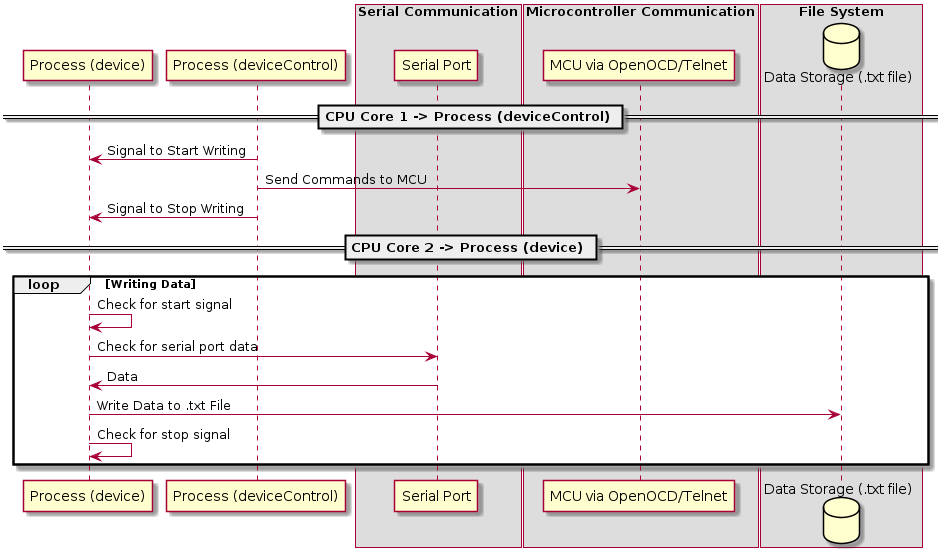
\includegraphics[width=1\textwidth, height=15cm]{~/Documents/Part_D_Modules/Individual_Project/Individual_report/figures/improved_process_design.png} % Adjust the path and width as needed
	\caption{The improved multi-processing design of the application. CPU Core 2 now allocates all the CPU time to sending commands to the MCU.}
	\label{fig:improved_application_design} % Use this label to reference the figure
\end{figure}

Results were collected using 4 \texttt{STM32F767ZI} MCUs for both of these solutions. In collaboration with Alex Henneman, results using the main setup(see figure ~\ref{fig:debate_fi_setup}) that utilised 36 MCUs running the second solution were also collected to verify the performance observed on the local setup. To collect benchmark data the application was run only once with varying number of boards and the run time was saved into a \texttt{.csv} file. The run time usually spanned in minutes thereby making multiple runs extremely time consuming, moreover the variation in run times was negligible unlike the applications in the first two objectives where the run times were in milliseconds and were more prone to variation. The benchmark collection strategy was similar to the one shown in figure ~\ref{fig:results_collection} except the application was run only once and the times were saved in a \texttt{.csv} file instead of a \texttt{.txt} file. 

\begin{figure}[htbp] % Positioning preference: here, top, bottom, page
	\centering
	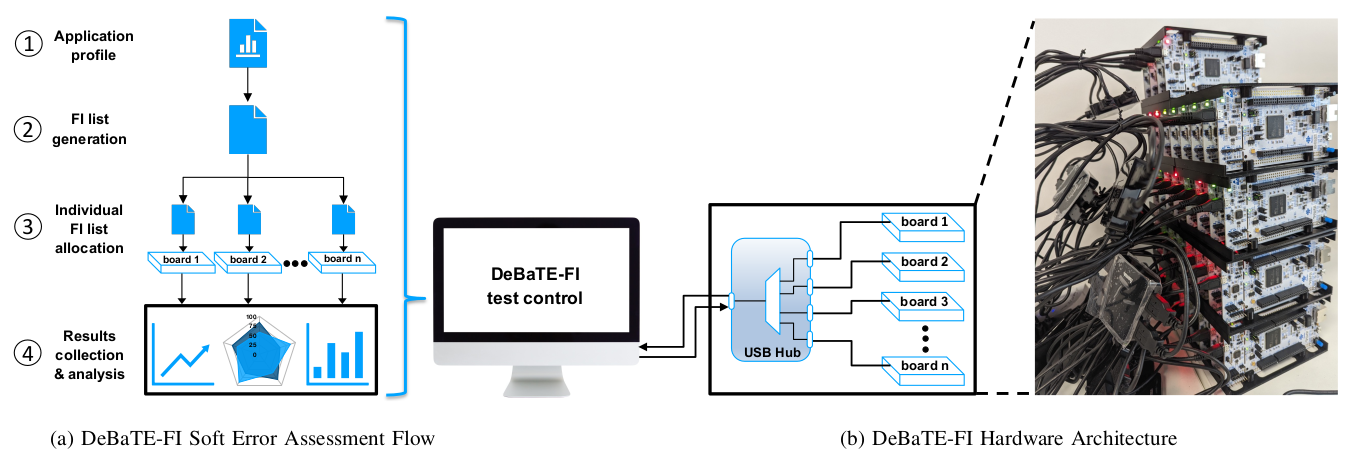
\includegraphics[width=1\textwidth, height=15cm]{~/Documents/Part_D_Modules/Individual_Project/Individual_report/figures/debate_fi_setup.png} % Adjust the path and width as needed
	\caption{\texttt{DeBaTE-FI} platform application on the main setup using 36 \texttt{STM32} boards\cite{debate_fi_publication}.}
	\label{fig:debate_fi_setup} % Use this label to reference the figure
\end{figure}

\chapter{Results and Discussion(8-10 pages)}
\section{Objective 1: \texttt{mpbenchmark}}

Results from the proposed solution collected from desktop(\texttt{x86} processor) are shown below, they are presented in the legend ``C++" and ``C++(SIMD Optimised)". A benchmark plot along with a speedup plot are shown in figures ~\ref{fig:mpbenchmark_desktop_plot} and ~\ref{fig:mpbenchmark_desktop_speedup_plot} respectively. 

\begin{figure}[htbp] % Positioning preference: here, top, bottom, page
	\centering
	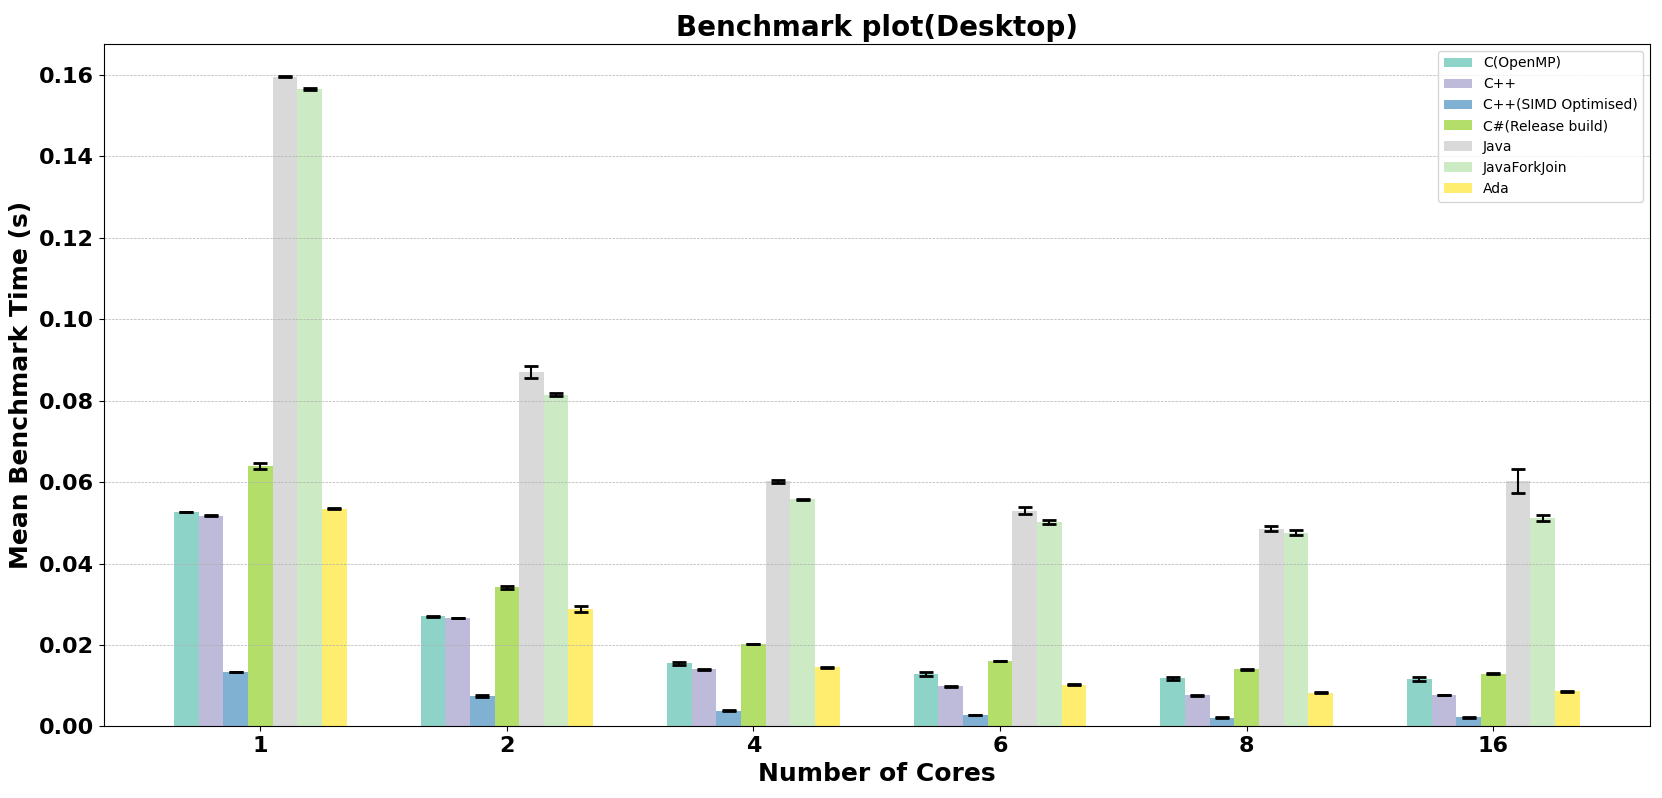
\includegraphics[width=1\textwidth, height=20cm]{~/Documents/Part_D_Modules/Individual_Project/Individual_report/figures/mpbenchmark_desktop.png} % Adjust the path and width as needed
	\caption{Mean benchmark plot of \texttt{mpbenchmark} collected from \texttt{x86} processor in seconds. The error bars represent 95\% confidence interval. (Lower is better).}
	\label{fig:mpbenchmark_desktop_plot} % Use this label to reference the figure
\end{figure}


\begin{figure}[htbp] % Positioning preference: here, top, bottom, page
	\centering
	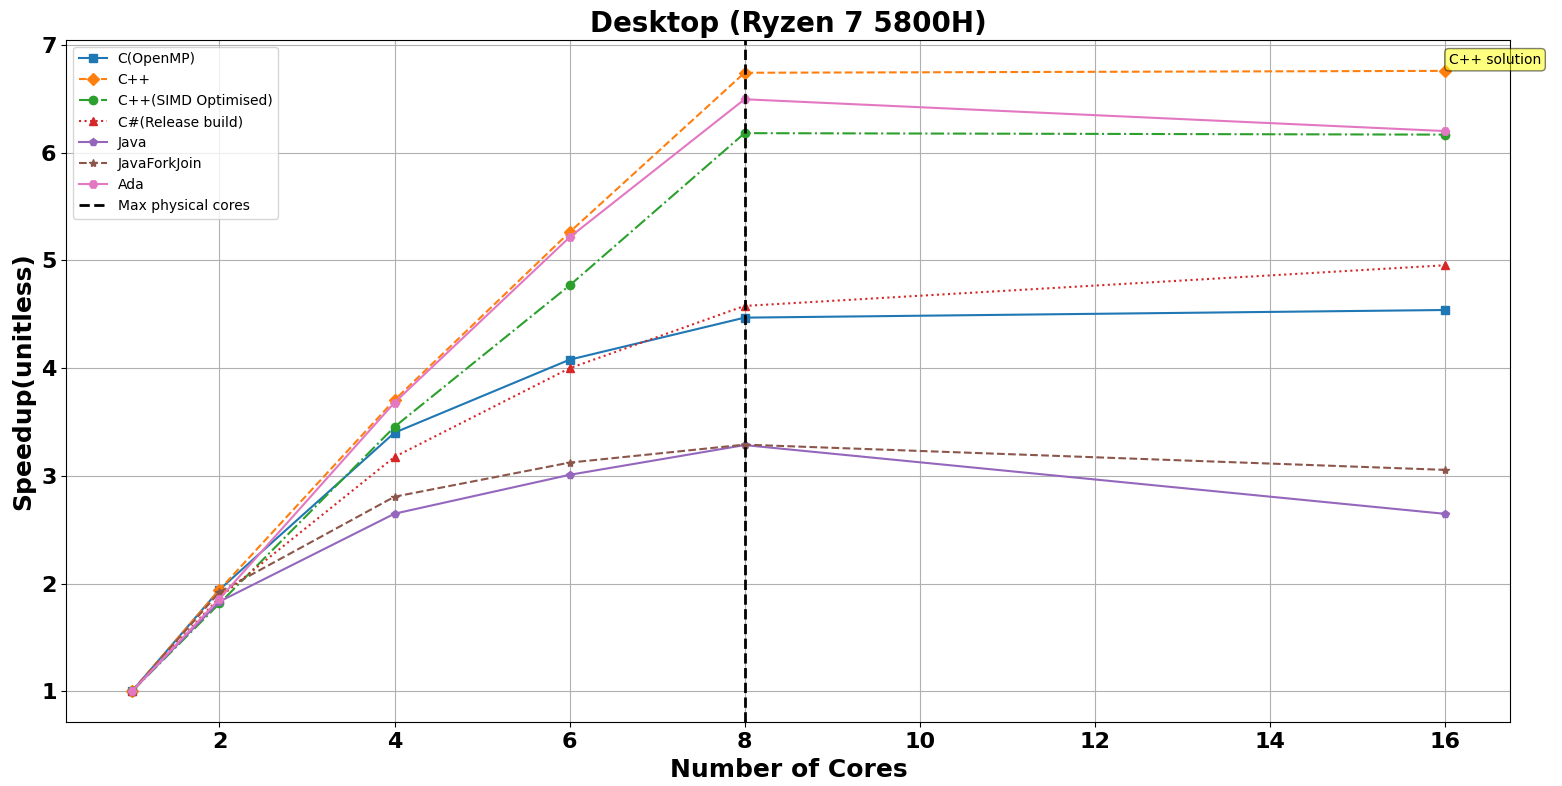
\includegraphics[width=1\textwidth, height=20cm]{~/Documents/Part_D_Modules/Individual_Project/Individual_report/figures/mpbenchmark_desktop_speedup.png} % Adjust the path and width as needed
	\caption{Speedup plot collected from \texttt{x86} processor. The vertical black line shows the maximum physical cores of the processor. (Higher is better).}
	\label{fig:mpbenchmark_desktop_speedup_plot} % Use this label to reference the figure
\end{figure}

On desktop(\texttt{x86}) processor, \texttt{AVX2} instructions were used to implement SIMD intrinsics therefore we compare the decimal precision with the original unoptimised SIMD code, see table ~\ref{tab:c++_avx2_pi}.

\begin{table}[htbp]
	\centering
	\begin{tabular}{|c|c|c|}
		\hline
		\textbf{Programming language/configuration} & \textbf{Decimal value of $\pi$} & \textbf{Mean run time using maximum threads(s)} \\ \hline
		\texttt{C++}             & 3.1415926535897643 &  0.007659 \\ \hline
		\texttt{C++/AVX2}   & 3.1415926535899033 &  0.002173  \\ \hline
		\texttt{C}                 & 3.1415926535897643 & 0.011577 \\ \hline
		\texttt{Ada}             & 3.1415926535897643 &  0.008623\\ \hline
	\end{tabular}
	\label{tab:c++_avx2_pi}
	\caption{Comparing the decimal precision of the \texttt{AVX2} enhanced solution with the original.}
\end{table}

% Talk about C++ solution outperforming the original in both run times and speedup 
% C++ SIMD enhanced outperformed even more with a lower speedup.
% Talk about SMT's benefits if any
% Discuss AVX2's decimal precision

The proposed \texttt{C++} solution outperformed the original implementations in \texttt{C} and \texttt{Ada} by over 11\%, marking a significant reduction in runtime. Additionally, it achieved a higher speed-up compared to the \texttt{Ada} solution, as illustrated in figure~\ref{fig:mpbenchmark_desktop_speedup_plot}. The SIMD-enhanced solution achieved a remarkable runtime reduction of over 70\%, significantly outperforming all other solutions. However, this version did not show as large a speedup when run with an increased number of threads, which is not surprising given the already low runtime with a single thread. Moreover, the \texttt{AVX2}-enhanced code demonstrated decimal precision up to 12 decimal places, with discrepancies appearing from the 13th decimal place onwards, as shown in table~\ref{tab:c++_avx2_pi}. This suggests a slight consideration that using \texttt{AVX2} instructions might lead to reduced precision for calculations requiring high decimal accuracy. However, the reduction in decimal precision has been minor, and its effects on the application have been largely inconsequential. Given the dramatic improvement in performance with \texttt{AVX2} instructions, the minor loss of decimal precision seems negligible compared to the benefits. Both solutions have met their objectives, with the first achieving superior speed-up and the second providing insights into CPU performance when SIMD intrinsics are utilized.

Another noteworthy observation is the lack of performance gain when scaling from 8 to 16 cores. The processor used supports simultaneous multi-threading (SMT), commonly branded as ``Hyper-threading" for Intel CPUs, which is typical in modern \texttt{x86} processors. SMT theoretically allows each physical core to execute two threads, and an 8-core processor with SMT would appear to have 16 cores. However, the proposed solutions, along with other compiled languages like \texttt{C} and \texttt{Ada}, showed negligible performance gains by utilizing the virtual cores. \texttt{Java} experienced a slight performance degradation, while \texttt{C\#} was the only language to demonstrate a performance increase. Using the results from the \texttt{x86} processor, we can conclude that the additional cores provided by SMT did not enhance performance and, in some cases, even degraded it.

Results obtained from the latest Raspberry Pi 5 (\texttt{Cortex A-76} processor) are shown in figures ~\ref{fig:mpbenchmark_rpi5_plot} and ~\ref{fig:mpbenchmark_rpi5_speedup_plot}. The results obtained from the Raspberry Pi 4(\texttt{Cortex A-72} processor) can be found in appendix (figures ~\ref{fig:mpbenchmark_rpi4_plot} and ~\ref{fig:mpbenchmark_rpi4_speedup_plot}).

\begin{figure}[htbp] % Positioning preference: here, top, bottom, page
	\centering
	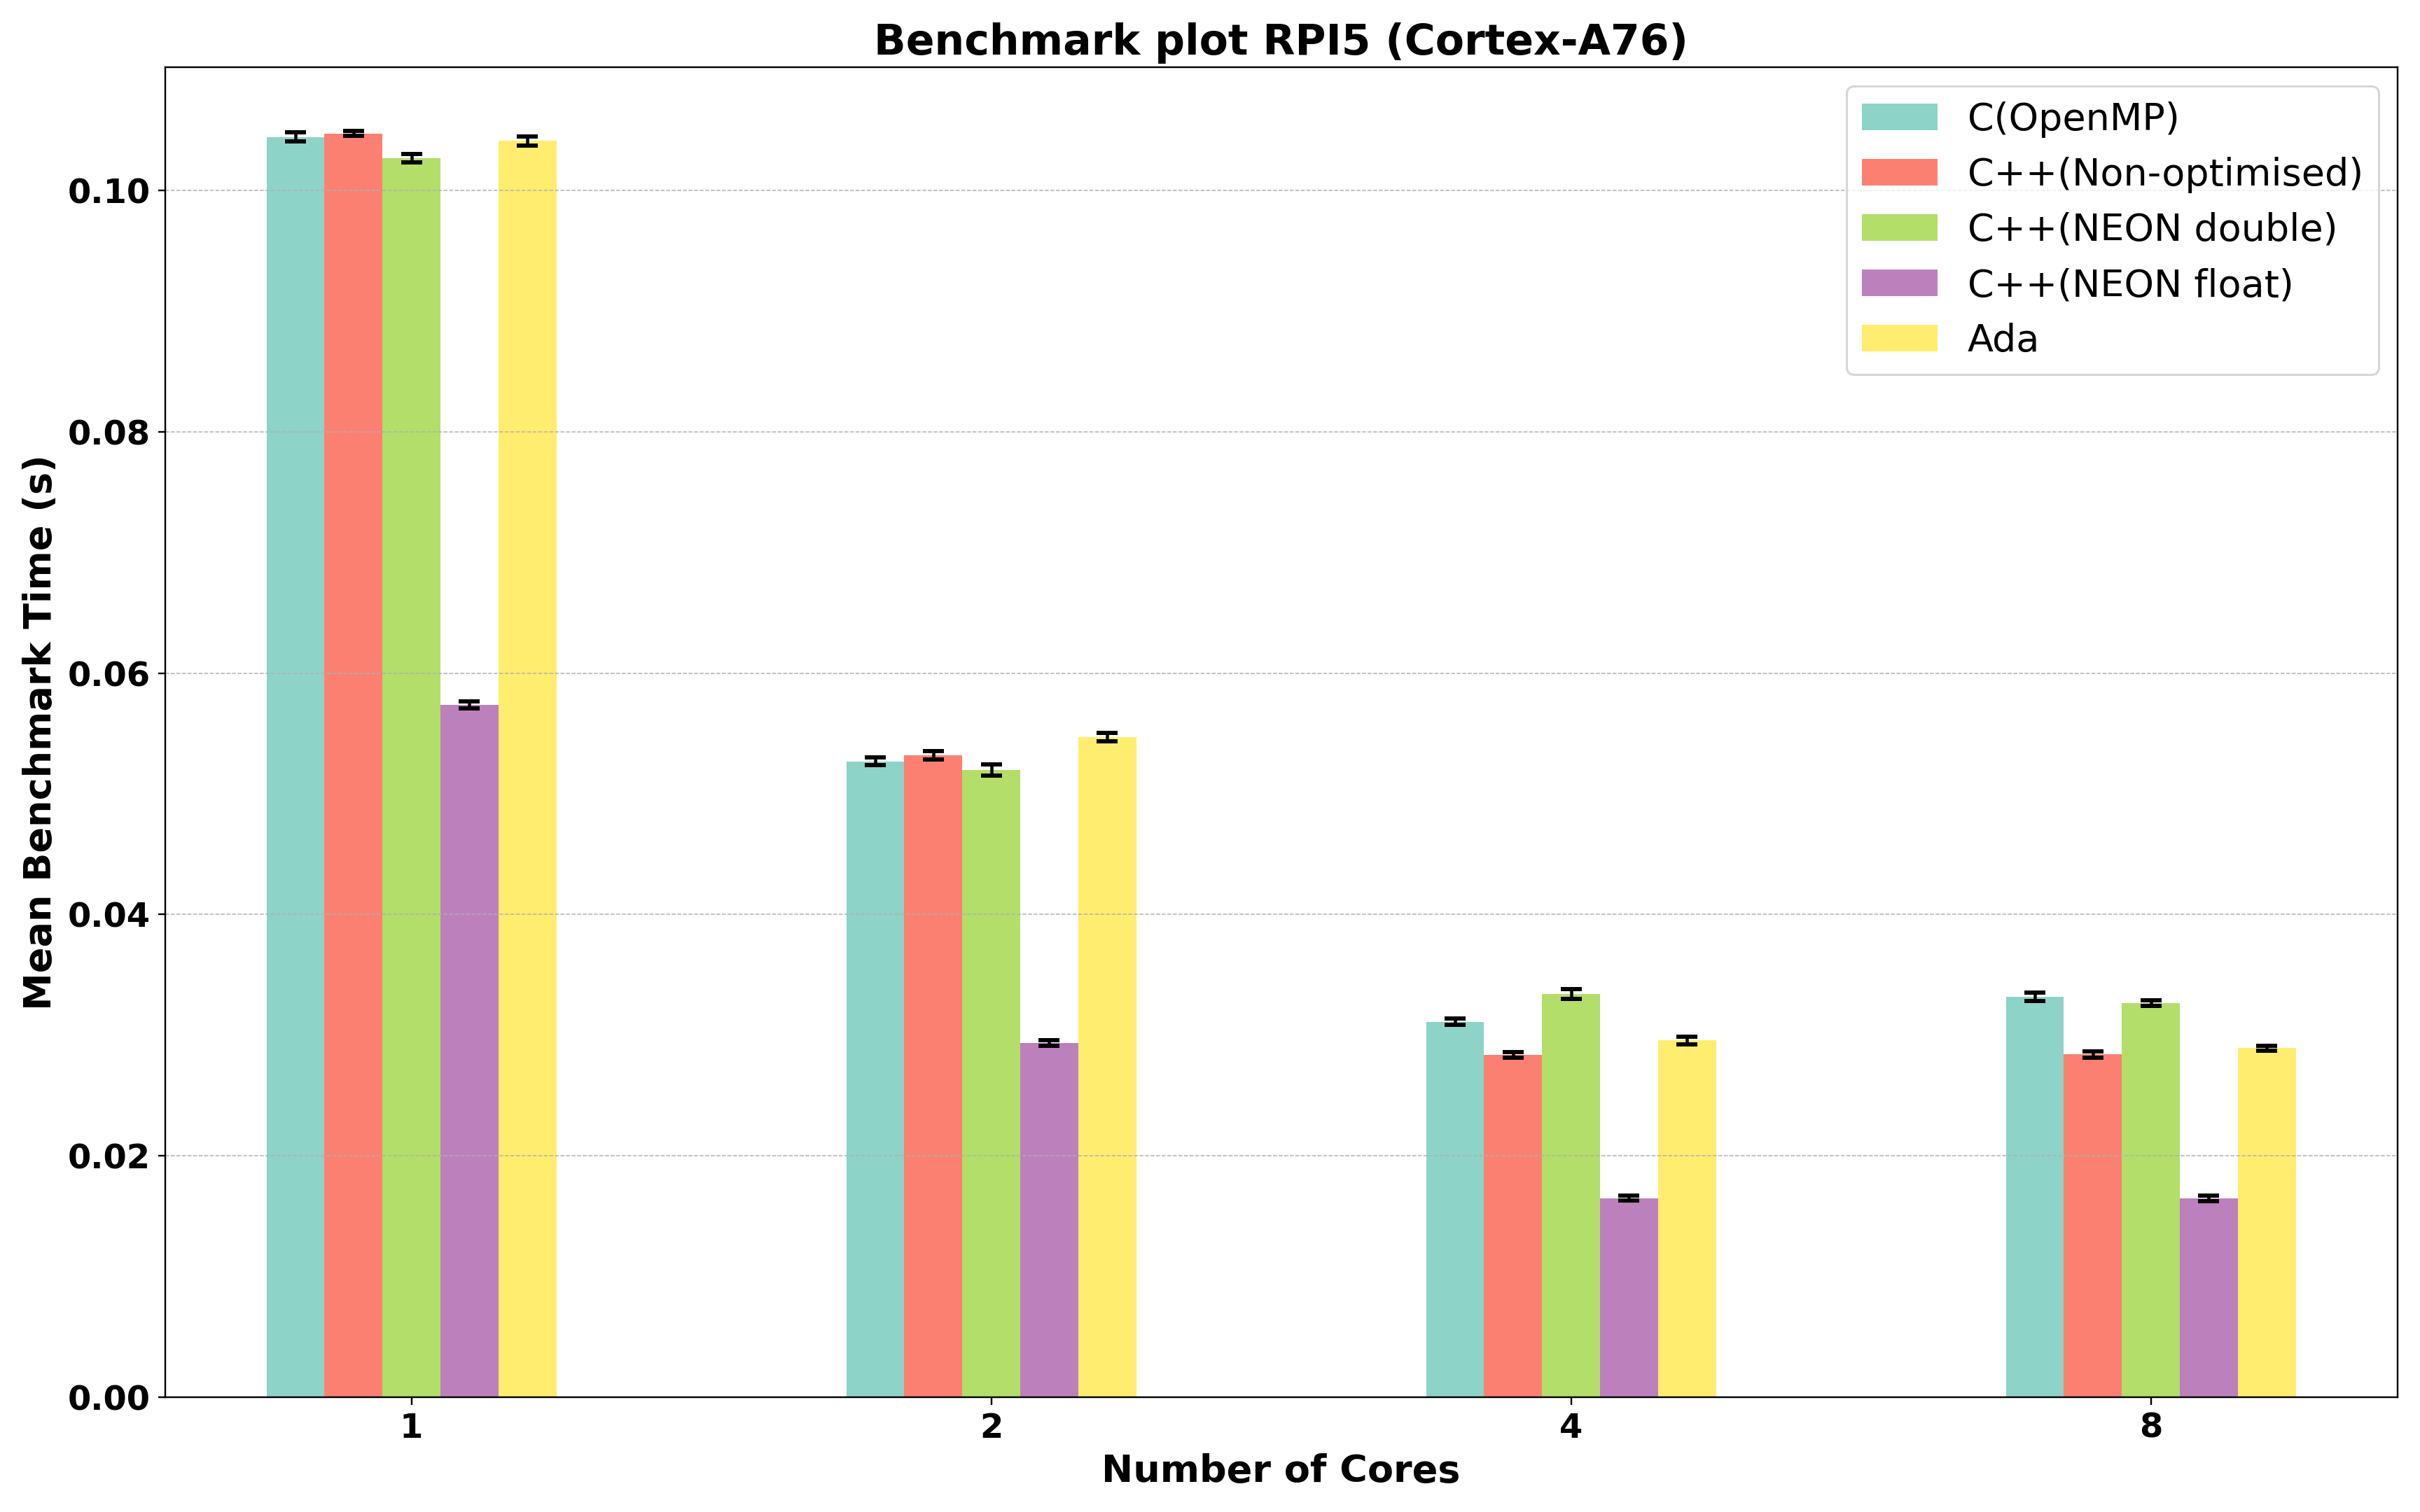
\includegraphics[width=1\textwidth, height=10cm]{~/Documents/Part_D_Modules/Individual_Project/Individual_report/figures/mpbenchmark_rpi5.png} % Adjust the path and width as needed
	\caption{Mean benchmark plot of results collected from Raspberry Pi 5(in seconds). The error bars represent 95\% confidence interval. (Lower is better).}
	\label{fig:mpbenchmark_rpi5_plot} % Use this label to reference the figure
\end{figure}

\begin{figure}[htbp] % Positioning preference: here, top, bottom, page
	\centering
	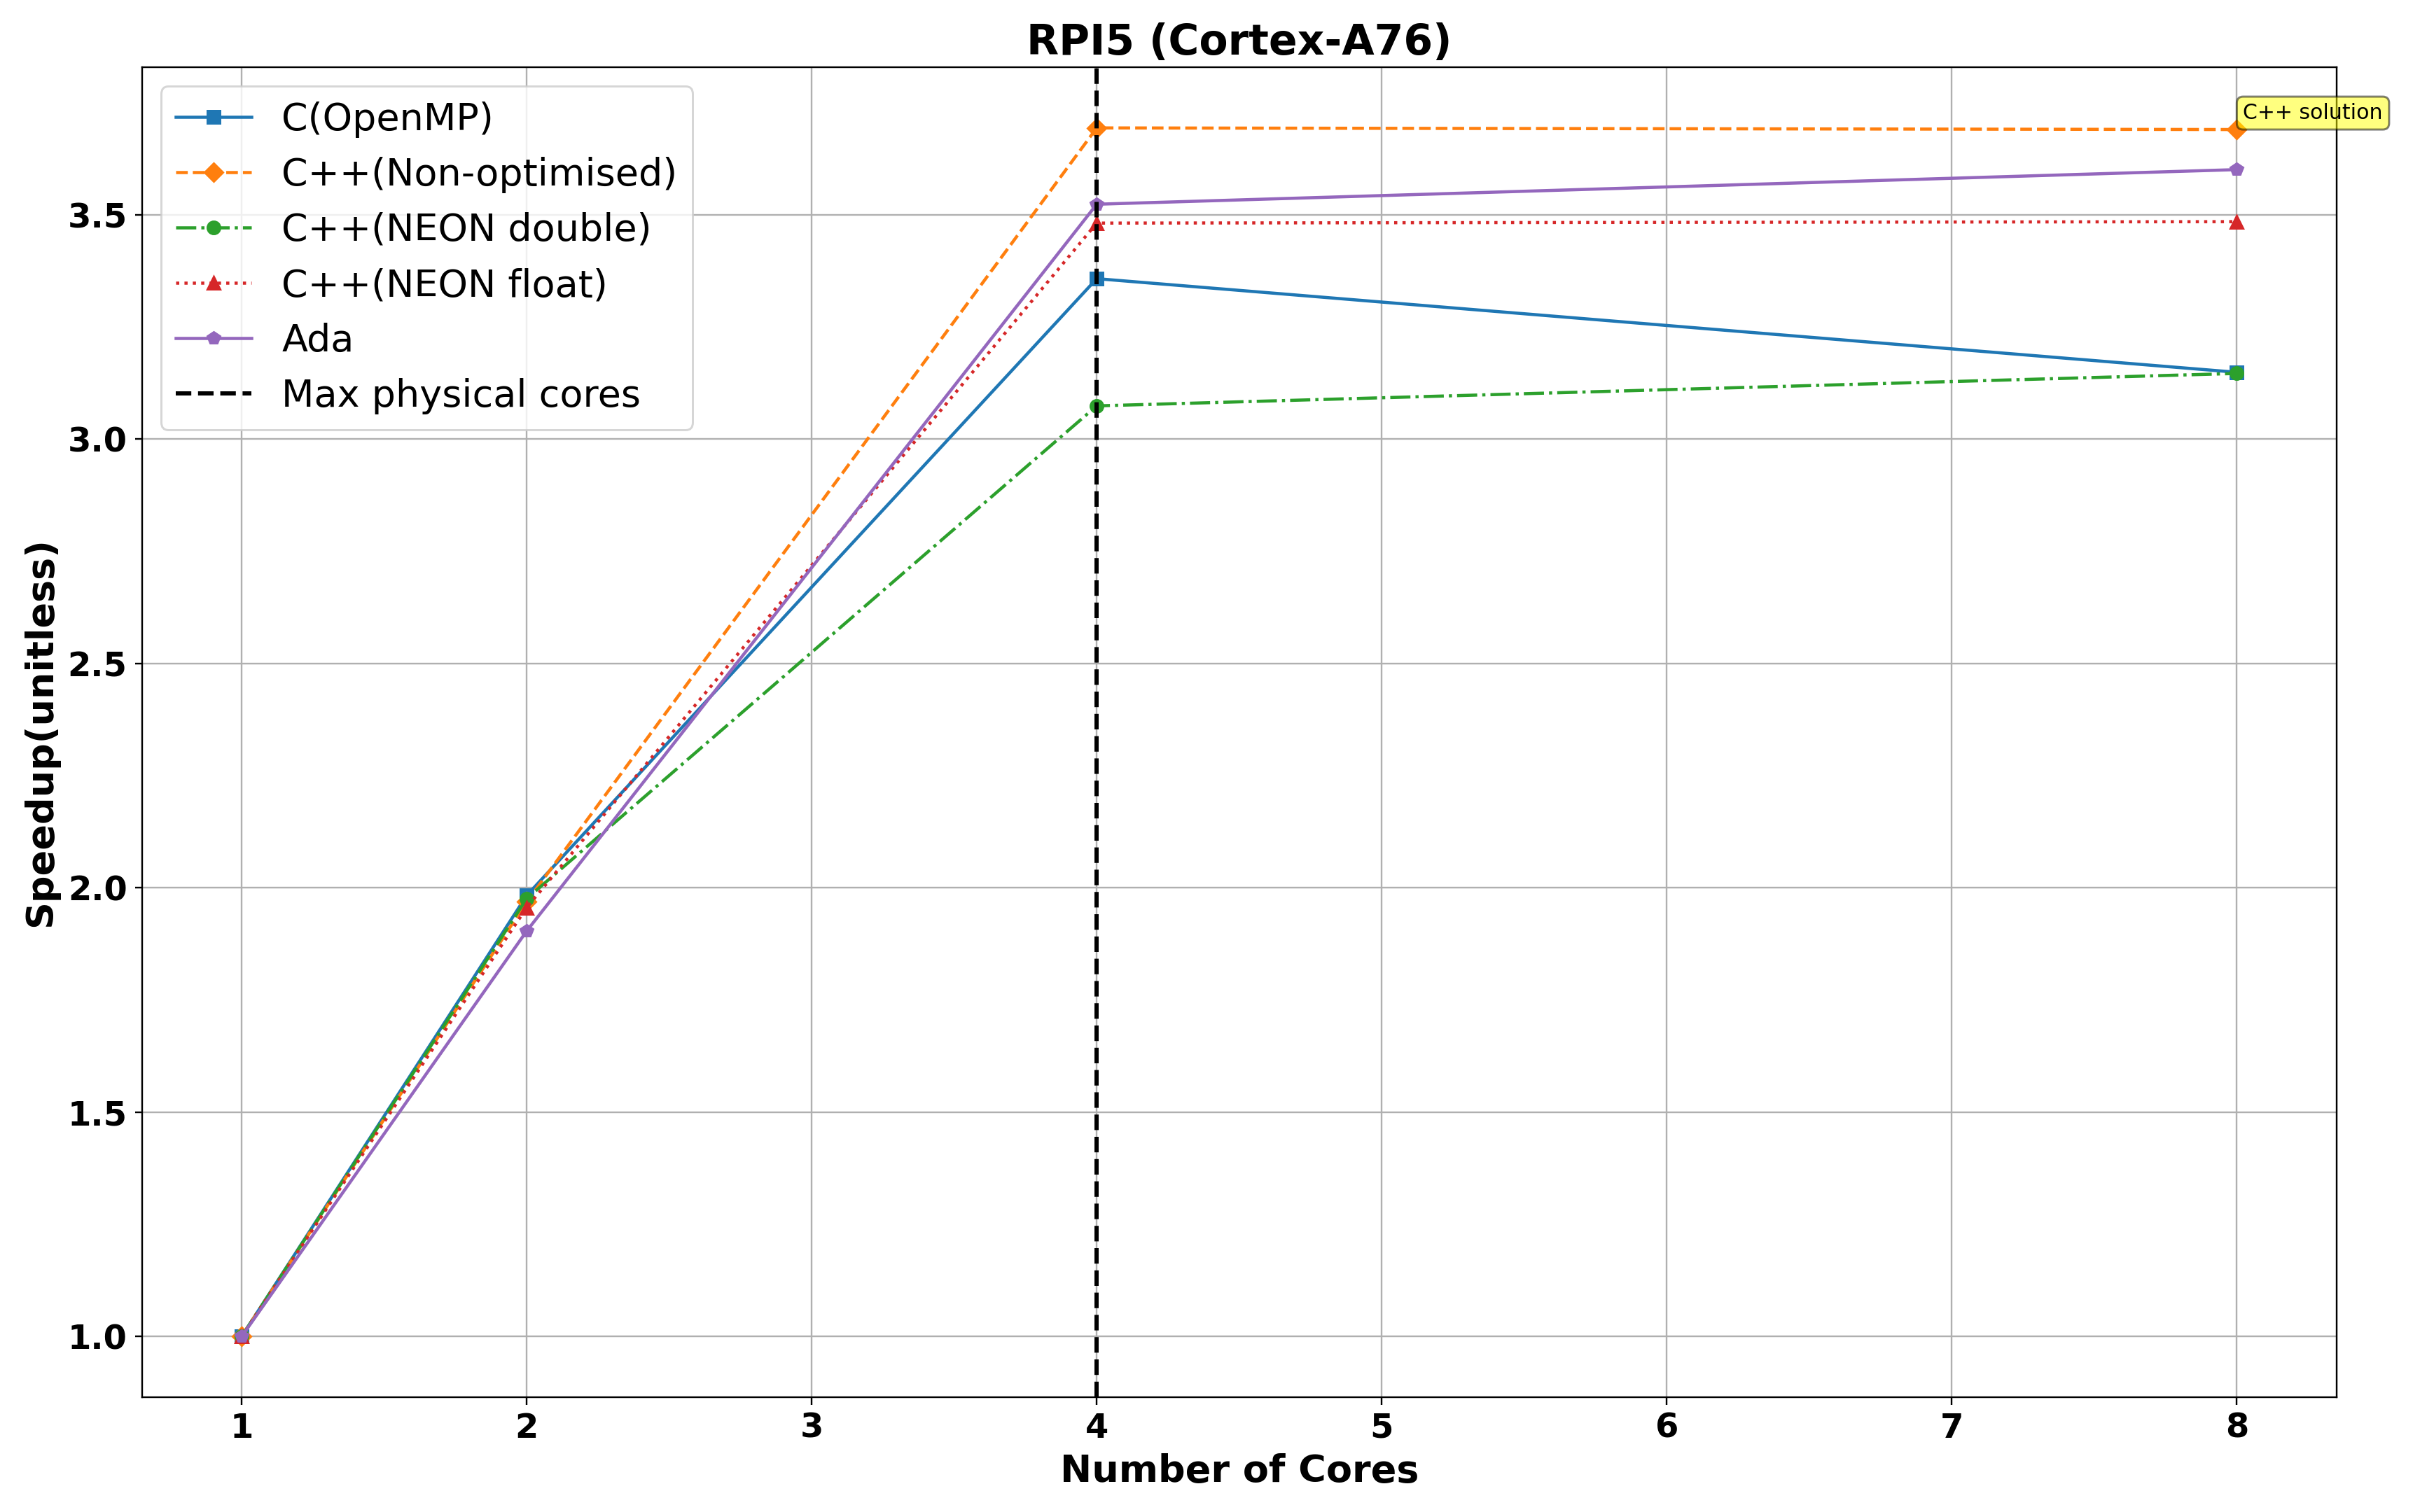
\includegraphics[width=1\textwidth, height=10cm]{~/Documents/Part_D_Modules/Individual_Project/Individual_report/figures/mpbenchmark_rpi5_speedup.png} % Adjust the path and width as needed
	\caption{Speedup plot collected from Raspberry Pi 5 processor. The vertical black line shows the maximum physical cores of the processor. (Higher is better).}
	\label{fig:mpbenchmark_rpi5_speedup_plot} % Use this label to reference the figure
\end{figure}

The decimal precision of using single and double precision floating point \texttt{NEON} instructions on the Raspberry Pi processors is compared in table ~\ref{tab:c++_neon_pi}.

\begin{table}[htbp]
	\centering
	\begin{tabular}{|c|c|c|c|}
		\hline
		\textbf{Programming language/configuration} & \textbf{Decimal value of $\pi$} & \textbf{Run time RPI5(s)} & \textbf{Run time RPI4(s)} \\ \hline
		\texttt{C++}                                                   & 3.1415926535897643 & 0.028356  & 0.115569 \\ \hline
		\texttt{C++/single-precision NEON}              & 3.141531467437744   &  0.016477 & 0.056352 \\ \hline
		\texttt{C++/double-precision NEON}             & 3.14159265358986     & 0.033399  & 0.116423 \\ \hline
		\texttt{C}                                                        & 3.1415926535897643 & 0.031107  & 0.116538\\ \hline 
		\texttt{Ada}                                                    & 3.1415926535897643  & 0.029549  & 0.117536 \\ \hline
	\end{tabular}
	\label{tab:c++_neon_pi}
	\caption{Comparing the decimal precision of the \texttt{NEON} enhanced solutions. RPI5 - Raspberry Pi 5, RPI4- Raspberry Pi 4. Mean benchmark time in seconds collected using maximum cores on the system(4 cores).}
\end{table}

% Talk about the proposed solution's performance in PI5 and PI4. 
% Talk about the speedup
% Talk about NEON solutions and their respective decimal precision.
% Can include the comparision with other solutions in the appendix, like Java and C# and Raspberry Pi 3 

The proposed solution outperformed both the \texttt{C} and \texttt{Ada} solutions in terms of runtime and speedup. On the Raspberry Pi 5, a slight reduction in runtime (about 4\%) and a notable improvement in speedup were observed. The results on the Raspberry Pi 4 were less impressive, showing only a 1\% improvement in performance and a marginal increase in speedup. Nevertheless, the proposed \texttt{C++} solution outperformed the original solutions in terms of runtime and speedup on both Raspberry Pi devices, although the improvement was marginal on the Raspberry Pi 4.

The \texttt{NEON} enhanced solutions using single precision floating-point produced over a 40\% reduction in time at the cost of lower speedup across threads and a reduced decimal precision to four decimal places. On the Raspberry Pi 5, the \texttt{NEON} solution using double precision failed to reduce runtime and produced the worst overall speedup across varying numbers of threads. On the Raspberry Pi 4, the \texttt{NEON} double precision solution did not reduce the runtime and produced a similar speedup to other solutions. However, the double precision solutions did offer far superior decimal precision, up to 12 decimal places. Given \texttt{NEON} instructions' reduced support for double precision floating points, developers must choose between single precision for significantly improved performance but lower decimal precision, and double precision, which did not improve performance on the tested embedded processors. These results are summarized in table~\ref{tab:c++_neon_pi}.

Benchmarks allow us to compare the latest Raspberry Pi 5 (\texttt{Cortex A-76}) against the older Raspberry Pi 4 (\texttt{Cortex A-72}). The \texttt{Cortex A-76} performed 75\% faster in terms of runtime when comparing the proposed \texttt{C++} solution, roughly \texttt{4x} faster. The \texttt{Cortex A-76} processor offered a 42\% reduction in runtime when \texttt{NEON(float)} enhanced code was used compared to a 51\% reduction in runtime for the \texttt{Cortex A-72}. Both processors exhibited a lower speedup when \texttt{NEON} instructions were used, similar to what was observed with the \texttt{x86} processor. The superior performance of the \texttt{Cortex A-76} may be attributed to a faster clock speed of 2.4 GHz compared to the 1.5GHz of the older \texttt{Cortex A-72} \cite{rasp_pi5_pi4_comparision}.

The proposed \texttt{C++} solution surpassed the previously developed \texttt{mpbenchmark}\cite{mpbenchmark_paper} on both \texttt{x86} and \texttt{ARM} processors. It offered better speedup across threads, and an alternate novel \texttt{SIMD} enhanced version (where the application decides whether to use \texttt{AVX2} or \texttt{NEON} depending on the processor type) can be utilized to analyse the CPUs' SIMD performance and scalability. This unprecedented improvement is part of an upcoming publication.

\section{Objective 2: \texttt{MobileNet}}
After parallelising \texttt{MobileNet} the results collected from desktop(\texttt{x86} processor) were compared with SIMD optimisations and without them. The benchmark and speedup plot are shown in figures ~\ref{fig:mobilenet_desktop_plot} and ~\ref{fig:mobilenet_desktop_speedup}. 

\begin{figure}[htbp] % Positioning preference: here, top, bottom, page
	\centering
	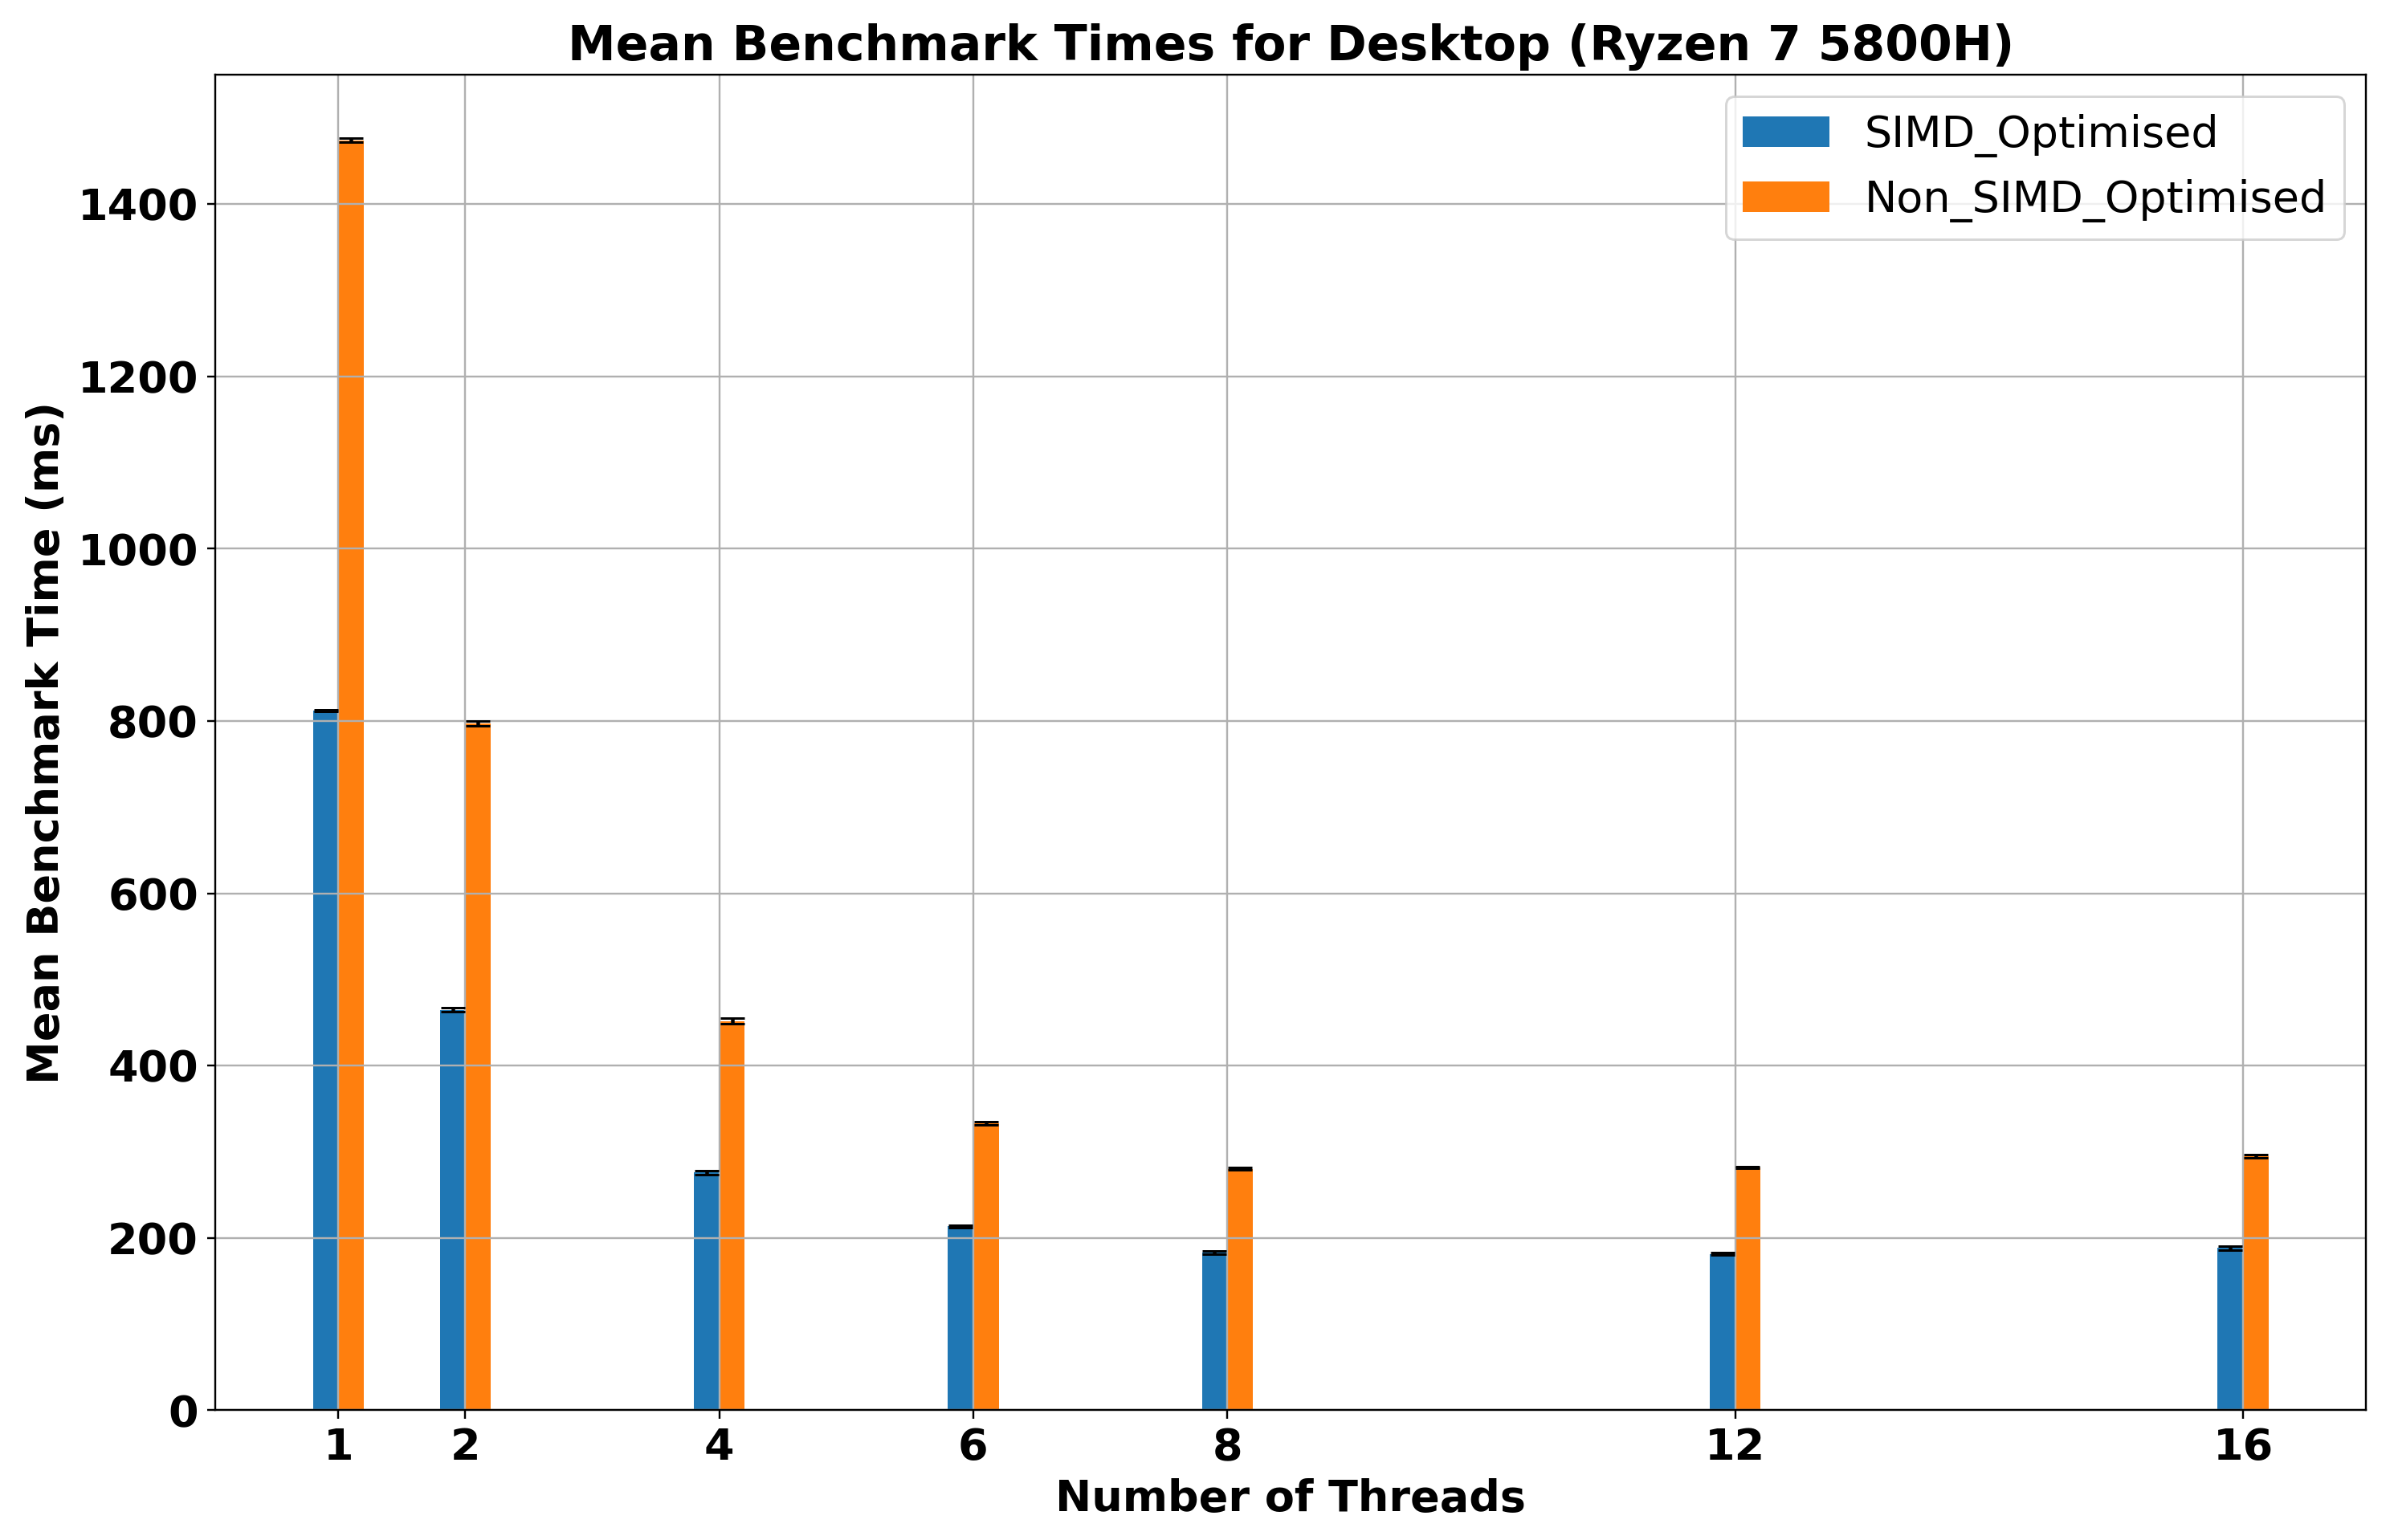
\includegraphics[width=1\textwidth, height=20cm]{~/Documents/Part_D_Modules/Individual_Project/Individual_report/figures/mobilenet_desktop.png} % Adjust the path and width as needed
	\caption{Mean benchmark plot of results collected from \texttt{x86} processor(in milliseconds). (Lower is better).}
	\label{fig:mobilenet_desktop_plot} % Use this label to reference the figure
\end{figure}

\begin{figure}[H] % Positioning preference: here, top, bottom, page
	\centering
	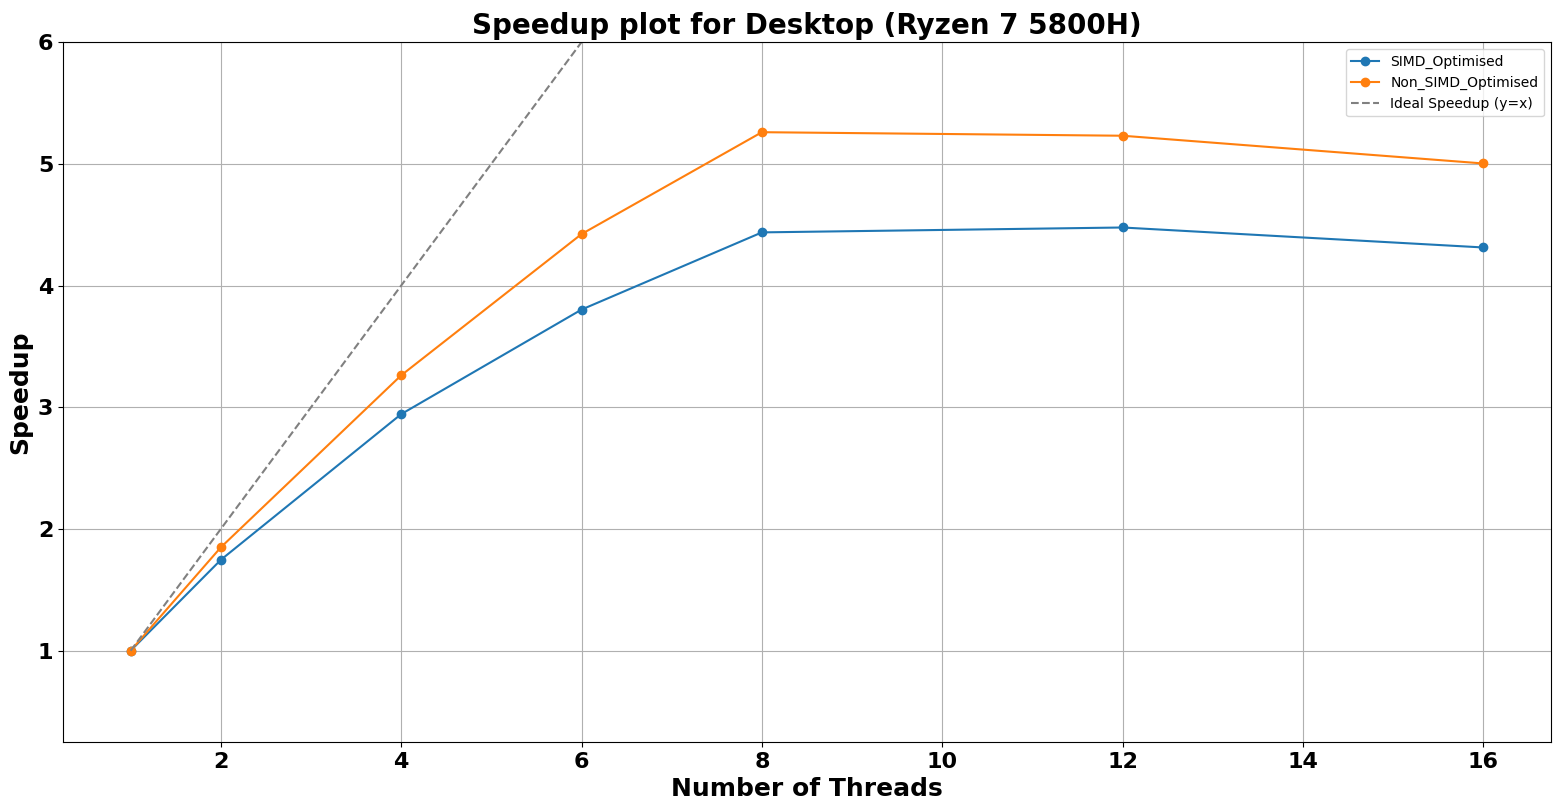
\includegraphics[width=1\textwidth, height=20cm]{~/Documents/Part_D_Modules/Individual_Project/Individual_report/figures/mobilenet_desktop_speedup.png} % Adjust the path and width as needed
	\caption{Speedup plot comparing the two solutions with results collected from \texttt{x86} processor. (Higher is better).}
	\label{fig:mobilenet_desktop_speedup} % Use this label to reference the figure
\end{figure}

The mean benchmark time of the original \texttt{MobileNet} application\cite{mobilenet_repo} was 1474.2 ms(using the \texttt{-O3} optimisation flag). The benchmark time using the maximum threads(16) with SIMD was 188.24ms and without SIMD it was 294.68ms. The SIMD optimisations are turned on and off as shown in listing  ~\ref{lst:mobilenet_parallel}. This presents a drastic reduction in run time of 87.2\% and 80.0\% for the SIMD and non-SIMD solutions respectively. Using multi-threading on the desktop processor yielded exceptional results and a dramatic improvement of the application. The results also indicate a performance degradation when using threads greater than 8 which is the maximum physical cores on the system. Both of the solutions produced a slight degradation of performance when going from 8 to 16 threads, suggesting once again the virtual cores from SMT did not yield in performance gains. 

The performance on the Raspberry Pi devices was a little more nuanced. The results of having different parallel regions and SIMD optimisations turned on or off were compared. The plots have the following legends:

\begin{enumerate}
	\item \texttt{3\_Parallel\_Regions\_SIMD}: all three functions \texttt{ConvLayer::forward}, \texttt{BatchNormalLayer::forward} and \texttt{ConvLayer::Addpad} have been parallelised with SIMD optimisations.
	\item \texttt{3\_Parallel\_Regions}: all three functions \texttt{ConvLayer::forward}, \texttt{BatchNormalLayer::forward} and \texttt{ConvLayer::Addpad} have been parallelised without SIMD optimisations.
	\item \texttt{2\_Parallel\_Regions\_SIMD}: only two functions \texttt{ConvLayer::forward} and \texttt{BatchNormalLayer::forward} have been parallelised with SIMD optimisations.
	\item \texttt{2\_Parallel\_Regions}: only two functions \texttt{ConvLayer::forward} and \texttt{BatchNormalLayer::forward} have been parallelised without SIMD optimisations.
\end{enumerate}

The results for Raspberry Pi 5 are shown in figures ~\ref{fig:mobilenet_rpi5_plot} and ~\ref{fig:mobilenet_rpi5_speedup}. The results for Raspberry Pi 4 can be found in appendix (figures ~\ref{fig:mobilenet_rpi4_plot} and ~\ref{fig:mobilenet_rpi4_speedup}). 

\begin{figure}[htbp] % Positioning preference: here, top, bottom, page
	\centering
	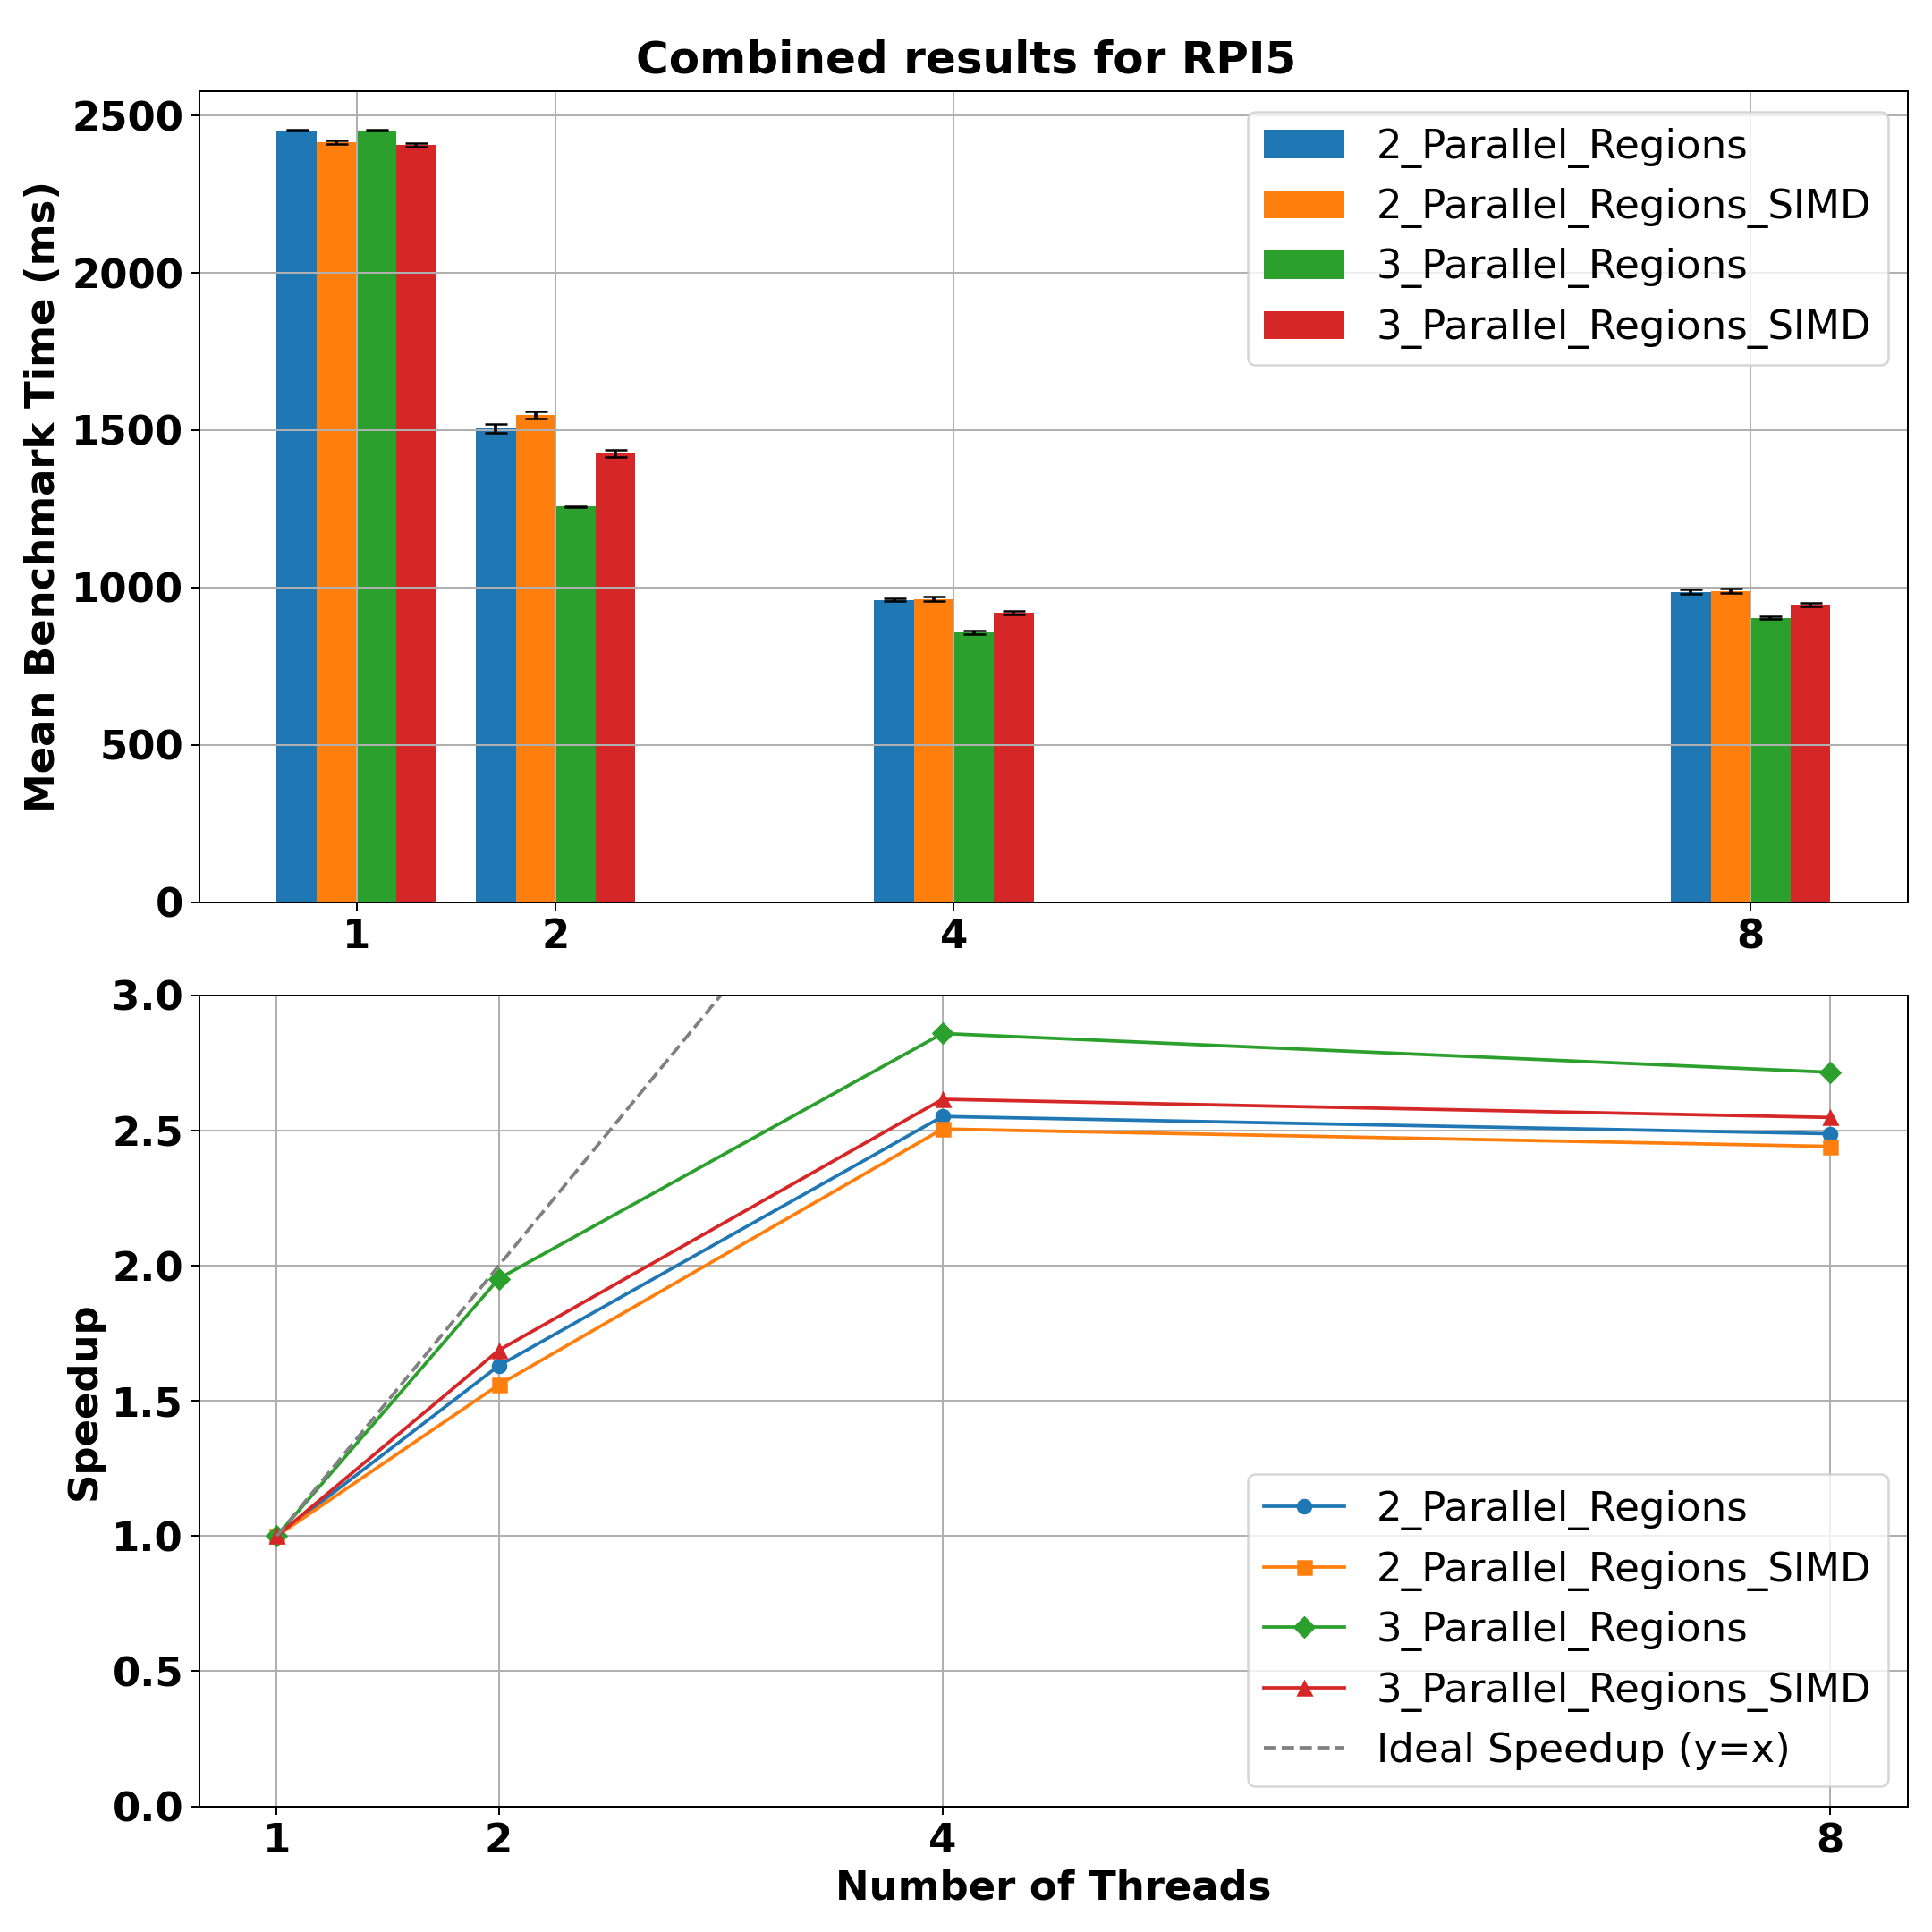
\includegraphics[width=1\textwidth, height=20cm]{~/Documents/Part_D_Modules/Individual_Project/Individual_report/figures/mobilenet_rpi5.png} % Adjust the path and width as needed
	\caption{Mean benchmark plot of results collected from \texttt{Cortex A-76} processor(in milliseconds). (Lower is better).}
	\label{fig:mobilenet_rpi5_plot} % Use this label to reference the figure
\end{figure}

\begin{figure}[htbp] % Positioning preference: here, top, bottom, page
	\centering
	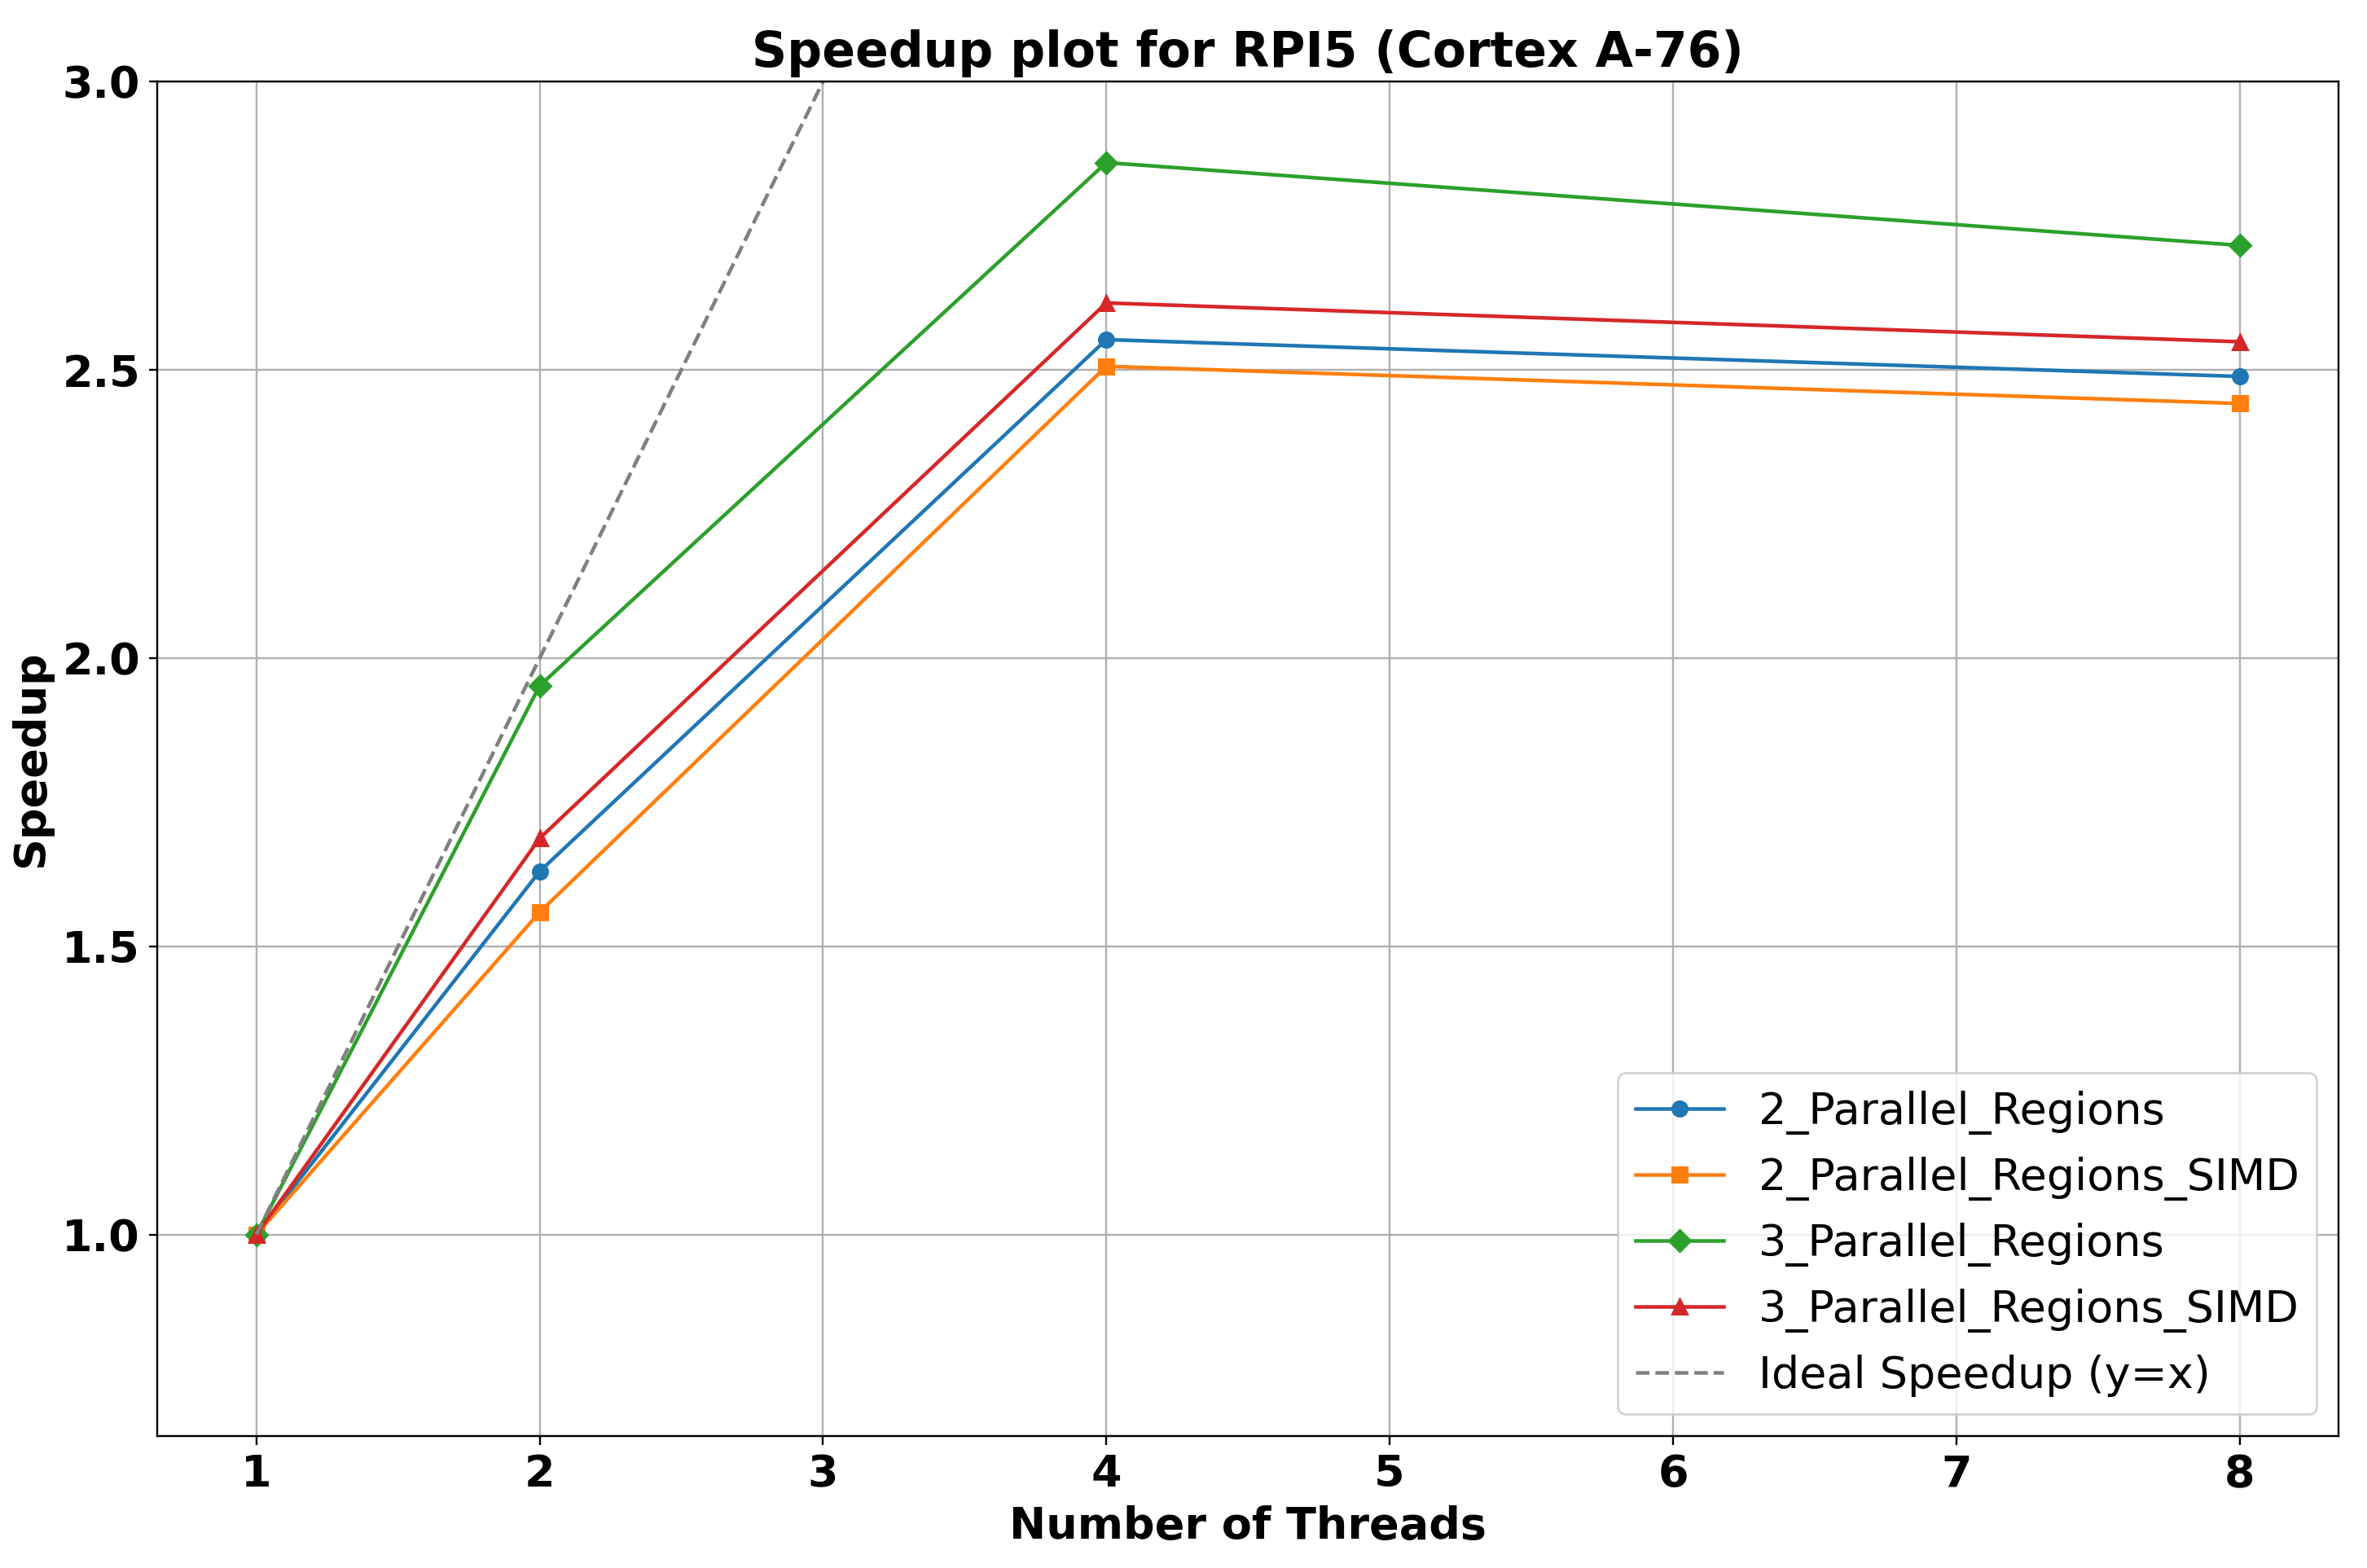
\includegraphics[width=1\textwidth, height=20cm]{~/Documents/Part_D_Modules/Individual_Project/Individual_report/figures/mobilenet_rpi5_speedup.png} % Adjust the path and width as needed
	\caption{Speedup plot comparing different solutions with results collected from \texttt{Cortex A-76} processor. (Higher is better).}
	\label{fig:mobilenet_rpi5_speedup} % Use this label to reference the figure
\end{figure}


\begin{table}[htbp]
	\centering
	\begin{tabular}{@{}lccc@{}}
		\toprule
		\textbf{Metric} & \textbf{Desktop} & \textbf{RPI5} & \textbf{RPI4} \\ \midrule
		% Row 1
		Original run time(ms)&1474.2&2462.33 &5108.77 \\
		% Row 2
		Lowest run time(ms)&188.24 &858.10 &2050.78 \\
		% Row 3
		Best speedup&5.26 &2.86 &2.79 \\
		% Row 4
		Optimal threads&8 &4 & 4\\
		% Row 5
		Performance gain versus original(\%)&87.2&65.2 & 59.90\\
		% Row 6
		Performance gain versus RPI4(\%)&90.8 &58.2 &0 \\
		\bottomrule
	\end{tabular}
	\caption{Comparing performance metrics across CPUs.}
	\label{tab:performance_comparison}
\end{table}

The results indicate that the optimal configuration for the Raspberry Pi 5 is \texttt{3\_Parallel\_Regions} without the use of SIMD optimisations. This resulted in the lowest run time and best overall speedup when compared to other configurations. For the Raspberry Pi 4 the results were harder to interpret, the lowest run time was achieved with \texttt{2\_Parallel\_Regions} but the best speedup was achieved with \texttt{2\_Parallel\_Regions\_SIMD}. Surprisingly SIMD optimisations on both of the Raspberry Pi devices did not result in a reduction in run time contrary to what was observed in objective 1. When comparing the two processors the \texttt{Cortex A-76} performed 58\% faster and offered the best performance with three parallel regions and also achieved a slightly better speedup(\texttt{2.86} versus \texttt{2.76}). Summarised results can be found in table ~\ref{tab:performance_comparison}. These results indicate that the \texttt{Cortex A-76} is better able to take advantage of parallelised regions. 

Contrasting to the Raspberry Pi devices the best performance on desktop was achieved with 3 parallel regions and SIMD optimisations. This presents an interesting challenge to the developer when porting this application on embedded devices, results collected from the Raspberry Pi devices showcase the need for tailoring the multi-threading architecture according to the target CPU to achieve optimal performance. Strangely the SIMD optimisations from the \texttt{OpenMP} library did not improve performance on the Raspberry Pi devices, this can be further investigated by manually implementing \texttt{NEON} instructions and compare its effects, similar to the method in objective 1. Both of the Raspberry Pi devices required slightly different configurations to achieve optimal performance. Optimal performance would be crucial in embedded processors part of drones and/or unnamed aerial vehicles(UAVs)\cite{drones_UAV_MLDL}. 

\section{Objective 3: \texttt{DeBaTE-FI} platform}
% First talk about the results collected from pc and using 4 STM32 boards 
% Explain the legend of the plots both run time and speedup 
% Then talk about the performance gain on the main setup 

Results collected from the local setup using four \texttt{STM32F767ZI} boards are shown in the following plots. The legend of the plots in in figures ~\ref{fig:debate_fi_plot} and ~\ref{fig:debate_fi_speedup} represent:

\begin{enumerate}
	\item \texttt{Original} : the unchanged \texttt{DeBaTE-FI} platform application. 
	\item \texttt{Python\_Optimised\_C++\_library} : the application with the optimised multi-processing design and using the \texttt{C++} \texttt{telnet} library.
	\item \texttt{Python\_Optimised} : the application with the optimised multi-processing design with the original \texttt{Python} \texttt{telnet} library.
	\item \texttt{Python\_Unoptimised\_C++\_library} : the application with the original architecture but with the \texttt{C++} \texttt{telnet} library.
\end{enumerate}

\begin{figure}[htbp] % Positioning preference: here, top, bottom, page
	\centering
	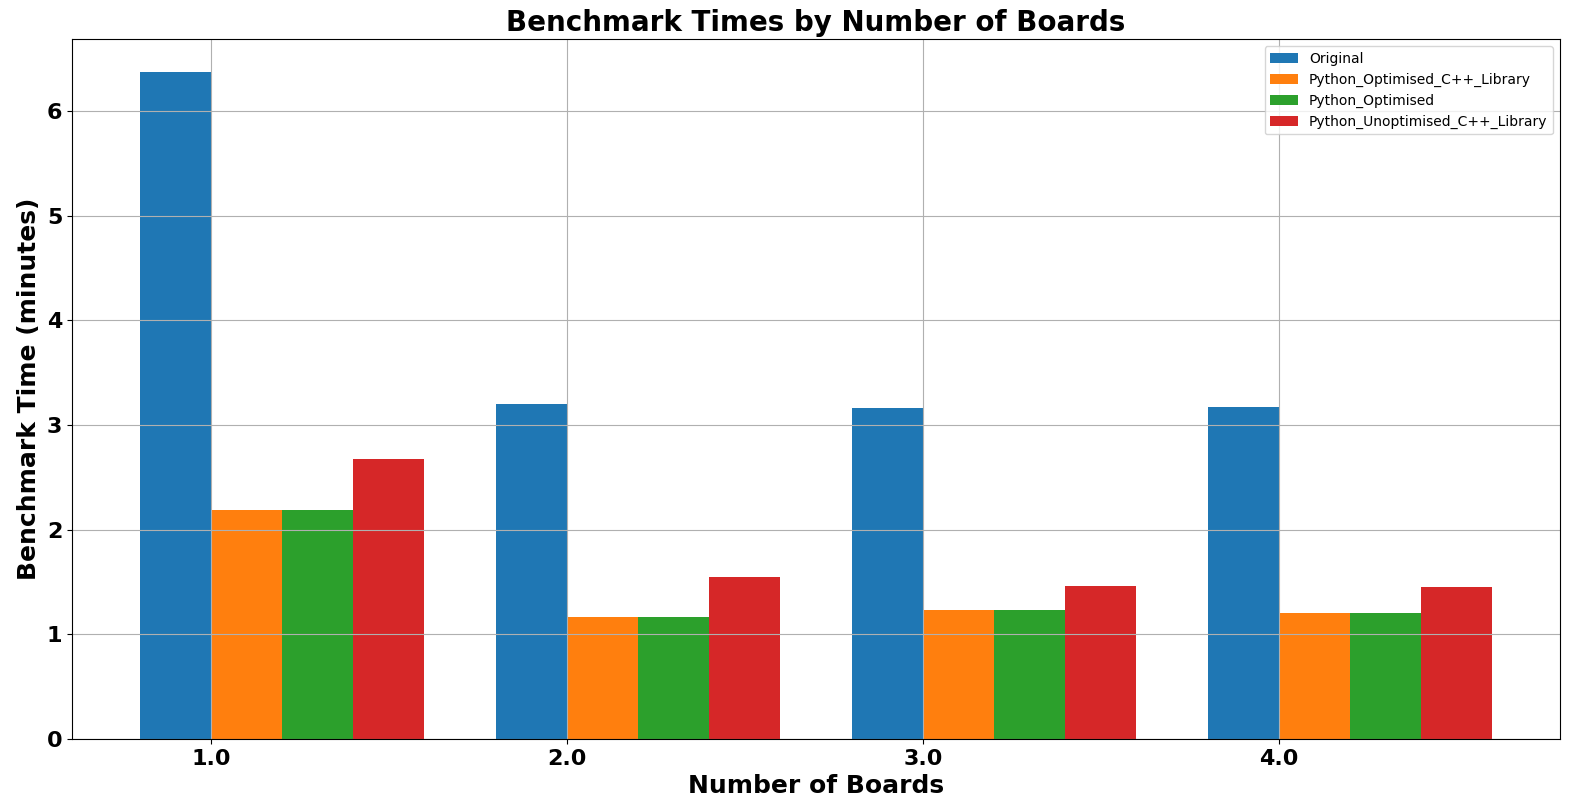
\includegraphics[width=1\textwidth, height=20cm]{~/Documents/Part_D_Modules/Individual_Project/Individual_report/figures/debate_fi.png} % Adjust the path and width as needed
	\caption{Benchmark plot comparing different solutions with runtime in minutes. (Lower is better).}
	\label{fig:debate_fi_plot} % Use this label to reference the figure
\end{figure}

\begin{figure}[htbp] % Positioning preference: here, top, bottom, page
	\centering
	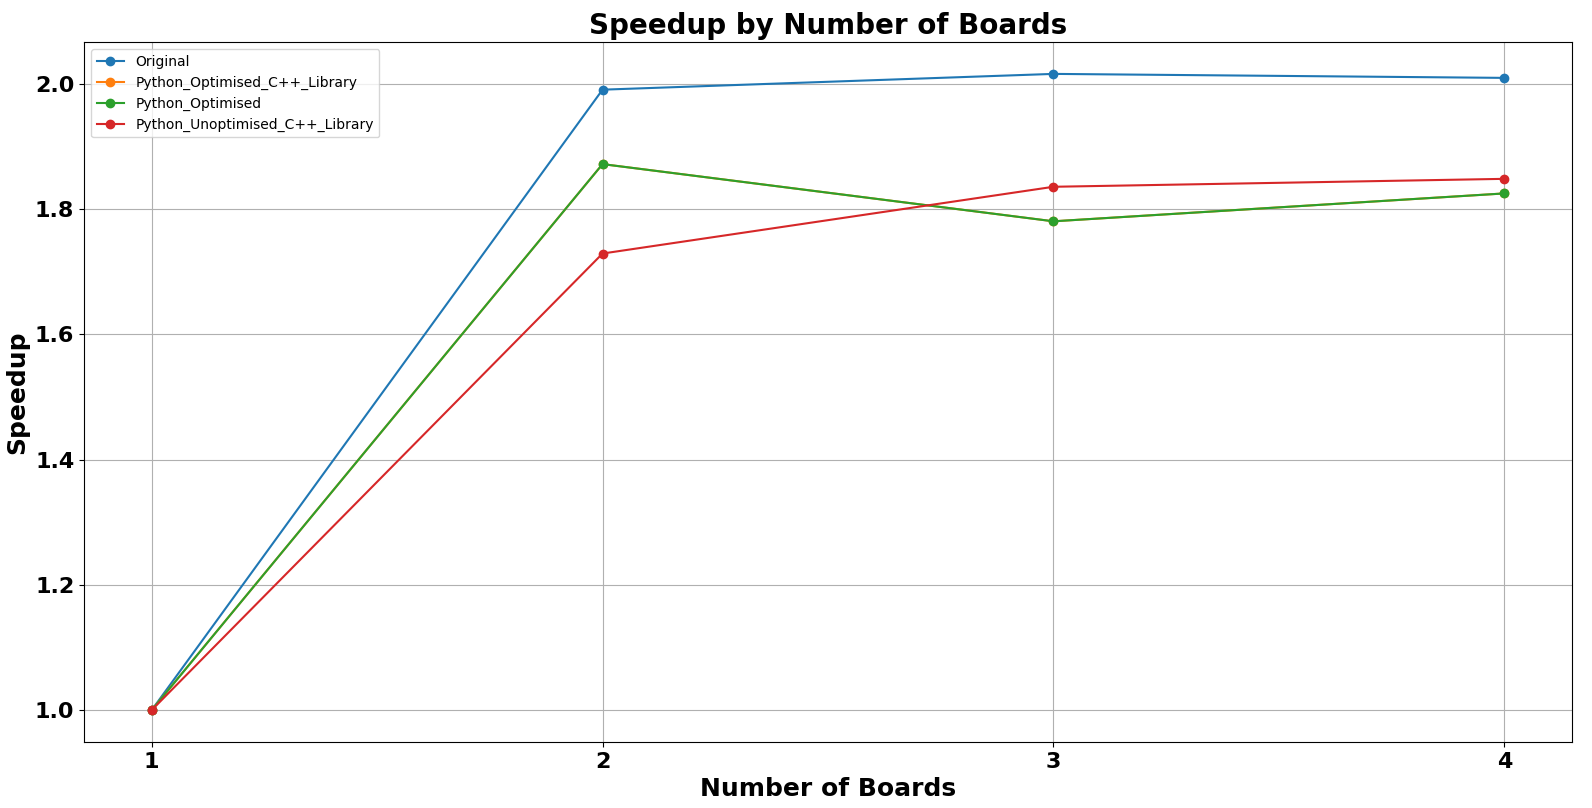
\includegraphics[width=1\textwidth, height=20cm]{~/Documents/Part_D_Modules/Individual_Project/Individual_report/figures/debate_fi_speedup.png} % Adjust the path and width as needed
	\caption{Speedup plot comparing the different solutions. (Higher is better).}
	\label{fig:debate_fi_speedup} % Use this label to reference the figure
\end{figure}

The \texttt{Python\_Unoptimised\_C++\_library} solution achieved a 55\% reduction in runtime, reducing it to 1.45 minutes from 3.17 minutes. However, it resulted in a lower speedup compared to the original, likely due to the limited runtime achieved using only one board. Conversely, the \texttt{Python\_Optimised} solution delivered the most substantial reduction in runtime of 62\% (1.20 minutes compared to 3.17 minutes). Despite this, it also exhibited a lower speedup, which began to degrade after the incorporation of 2 boards. These results were derived from only 5 test scenarios to mitigate the prolonged runtime of the application. The findings indicate that the \texttt{Python\_Optimised} solution reached a plateau, showing no further improvements beyond the use of 2 boards. This plateau may be attributed to the limited runtime where adding additional boards did not yield performance gains, suggesting that the optimal performance with this improved solution can be achieved using only 2 boards instead of 4.

Surprisingly, no significant performance improvement was observed with the \texttt{Python\_Optimised\_C++\_library} solution. Given previous results, one might expect that integrating the \texttt{C++} library into the application would enhance performance, and that optimizing the multiprocessing design would further boost efficiency. Combining the two was anticipated to yield an even larger performance increase, yet this did not occur. In the \texttt{Python\_Optimised} solution, adding the \texttt{C++} library did not enhance performance; in fact, the performance was identical to when the \texttt{C++} library was not included. This outcome raises an intriguing question: why did only the original \texttt{DeBaTE-FI} platform benefit from integrating the \texttt{C++} library, while no performance gain was observed when the \texttt{C++} library was incorporated into the \texttt{Python\_Optimised} solution? Investigating this discrepancy will be crucial for future efforts to further optimize the software.

All three developed solutions significantly improved the performance of the \texttt{DeBaTE-FI} platform. The \texttt{Python\_Optimised} solution is particularly convenient as it eliminates the need to compile the \texttt{C++} code into a shared library (\texttt{.so}) file. The \texttt{C++} class can be used in the application as the standard \texttt{telnet} library, replacing the older \texttt{Telnetlib} \texttt{Python} library which was deprecated in \texttt{Python 3.11} and is slated for removal in version \texttt{3.13}\cite{PythonTelnetlib}. Additionally, the \texttt{C++} library facilitates the creation of custom functions and allows for prioritization of performance. Therefore, this project proposes the use of the newly developed \texttt{C++} library (\texttt{Telnetlibcpp}) when the \texttt{DeBaTE-FI} platform's code is updated to accommodate later versions of \texttt{Python}.

Results from the main setup (figure~\ref{fig:debate_fi_setup}) using the \texttt{Python\_Optimised} solution are presented in table~\ref{tab:debate_metrics}. A 43.5\% performance gain was observed, compared to the 62.1\% improvement noted in the local setup. This still represents a significant enhancement in performance. To further investigate the proposed solution, it would be beneficial to analyse results using a varying number of boards and their respective speed-ups in the main setup. This analysis could help determine the ideal number of boards for optimal performance. Additionally, no results were collected using single-board computers (SBCs) like the Raspberry Pi, primarily due to the time constraints of this project. Investigating the performance of the proposed solution on SBCs could be another valuable area of exploration.

\begin{table}[htbp]
	\centering
	\begin{tabular}{@{}lcc@{}} % 'l' for left-aligned text, 'c' for centered text
		\toprule
		\textbf{Metric} & \textbf{Local setup} & \textbf{Main setup} \\
		\midrule
		\texttt{STM32} Test Boards & 4 & 36 \\
		Test scenarios & 5 & 1000 \\
		Original solution run time(min) & 3.17 & 234.47 \\
		Optimised solution run time(min) & 1.20 & 132.4 \\
		Performance improvement(\%) & 62.1 & 43.5 \\
		\bottomrule
	\end{tabular}
	\caption{Comparison of benchmark metrics on the local versus the main setup(figure~\ref{fig:debate_fi_setup}).}
	\label{tab:debate_metrics}
\end{table}


\chapter{Conclusion(2 pages)}
% Your conclusion content here.
% commentary and interpretation of the main outcomes or findings, relative significance of findings, implications of results, limitations and future work.

% mpbenchmark: novel solution, C++ and SIMD suitable for both desktop and embedded processors to assess multi-core performance. State of the art acheivement, limitation would be how short the application is for more high-end CPUs. Future work could involve having a larger portion of application benchmark. SMT failed to deliver performance on x86 processor.

The first objective was met with strong results, surpassing the initial aim. A novel benchmark was developed using modern \texttt{C++}, which exceeded the capabilities of the previous \texttt{mpbenchmark}\cite{mpbenchmark_paper} in several aspects especially those implementations in \texttt{C} and \texttt{Ada}. The novel software design was modular and object-oriented, enhancing scalability. An alternate solution was also developed to assess CPU performance using SIMD intrinsics, with the application automatically selecting \texttt{AVX2} or \texttt{NEON} based on the CPU type. Results from desktop (\texttt{x86}) processors indicated negligible performance gains when utilizing SMT (or Intel's ``Hyper-threading"). The latest Raspberry Pi 5, equipped with the \texttt{Cortex A-76} processor, significantly outperformed the older Raspberry Pi 4's \texttt{Cortex A-72} by 75\%. On \texttt{ARM}-based CPUs, using single-point decimal precision with \texttt{NEON} instructions resulted in a 42-51\% performance gain but limited precision to four decimal places, posing a trade-off between performance and decimal precision.

Future research and development would focus on enhancing the benchmark to include more complex and demanding calculations to better assess the performance of high-end CPUs. The \texttt{x86} processor used in this project completed the benchmark application in less than 10 milliseconds, which might lead to a slightly misleading assessment of CPU capabilities if the application is too simplistic, despite utilizing multiple threads. While this benchmark is effective for testing on embedded processors, it may be insufficient for assessing the performance of modern high-end CPUs, which now often feature more than 10 physical cores.

% MobileNet: novel solution and a dramatic performance boost. Desktop SMT failed to deliver again. On embedded devices need to tailor the solution to the target CPU. Limitation would be to improve the MobileNet to include the usage of modern C++ features. Future work would involve investigating SIMD optimisation on embedded/ARM CPUs for optimal performance. 
The second objective achieved novel results. The popular image classification algorithm \texttt{MobileNet}\cite{mobilenet_paper}\cite{mobilenet_repo} was parallelized using the \texttt{OpenMP} library. This optimized application provided a substantial 87\% reduction in runtime on the test \texttt{x86} processor when all system threads were utilized, though SMT did not yield any performance gains. On Raspberry Pi devices, performance improvements were more complex, and optimal performance was achieved when the application's multi-threaded architecture was specifically tailored to the target CPU. The optimized \texttt{MobileNet} application saw performance gains of 59.9\% and 65.2\% on Raspberry Pi 4 and 5, respectively, when all system threads were employed. However, the use of SIMD optimizations on the Raspberry Pi devices did not result in a significant performance improvement. In terms of application runtime, the latest Raspberry Pi 5 outperformed the Raspberry Pi 4 by 58\%. Furthermore, the optimal configuration on the Raspberry Pi 5 involved utilizing three parallel regions of the application instead of only two on the Raspberry Pi 4, indicating that the \texttt{Cortex A-76} processor is better suited to exploit the \texttt{OpenMP} library's parallel regions.

Future work would focus on improvements to the \texttt{MobileNet} application’s software design. Enhancements could aim to increase modularity and leverage modern \texttt{C++} features. Another area for investigation is to determine why the \texttt{OpenMP} library's SIMD clause did not yield performance gains. This could be explored by manually employing \texttt{NEON} instructions and benchmarking the application to analyse the effects.

% DeBate-FI: unprecendented performance improvement in both local setup and the main setup. Limitation would redesigning the code of the application to make it more modular. Future work would be to collect more results from the main setup and use the C++ library instead of the Python obsolete telnet library. 
The third objective, the most challenging of all, was also met with strong results, achieving and even surpassing the initial aims. The \texttt{DeBaTE-FI} platform's application software, specifically its multiprocessing and multithreading capabilities, was optimized to reduce runtime and enhance scalability. The optimised solution successfully reduced runtime by 62.1\% in the local setup. In the main setup, the optimized solution achieved a 43.5\% reduction in runtime, confirming that the performance improvements are consistent beyond the local environment. Both results demonstrate significant and unprecedented improvements in performance. Additionally, an alternative solution was developed, which involved integrating an open-source \texttt{C++} library into the \texttt{Python} application for \texttt{telnet} communication. This solution also showed strong performance gains in the local setup, though not as substantial as the optimized \texttt{Python} solution, and it was not tested in the main setup due to project time constraints. However, the developed \texttt{C++} library can replace the existing, obsolete \texttt{Python} \texttt{telnetlib} library currently used by the \texttt{DeBaTE-FI} platform. Thus, this project not only enhanced the performance of the \texttt{DeBaTE-FI} platform but also offers a high-performance library that can be integrated into the \texttt{DeBaTE-FI} platform to replace its existing \texttt{telnet} library.

Future work would involve collecting more detailed results using the main setup to further analyze the optimized solution's performance. This task is time-consuming due to the long runtime of this application. Another area worth researching is the optimization of the application's design, which currently remains convoluted and challenging to enhance, fix bugs, and potentially discover further optimizations for improved performance. The project also proposes using the developed \texttt{C++} library for \texttt{telnet} communication to replace the application's soon-to-be deprecated \texttt{telnetlib} \texttt{Python} library.


% Ensure bibliography starts on a new page and add it to the ToC.
\clearpage % Ensures bibliography starts on a new page.
\phantomsection % Ensures that the hyperlink anchor is correctly placed here.
\addcontentsline{toc}{chapter}{References}
\bibliographystyle{IEEEtran}
\bibliography{references} % Assumes your bibliography is in the 'references.bib' file.

% Ensure appendices start on a new page and add it to the ToC.
\newpage
\chapter{Appendices(Not completed)}
\begin{appendices}
	\section{System and Raspberry Pi specifications}
\label{sec:sysetm_specs}

The following setup was used to collect results and benchmarking data:

\begin{table}[htbp]
	\centering
	\begin{tabular}{@{}lccc@{}}
		\toprule
		\textbf{Specification} & \textbf{Desktop} & \textbf{RPI5} & \textbf{RPI4 Model B} \\ 
		\midrule
		Processor             & AMD Ryzen 7 5800H & Cortex A-76 & Cortex A-72 \\
		Processor Type          & x86                      & ARM            & ARM \\
		Processor Speed        & 3.2 - 4.4 GHz       & 2.4 GHz       & 1.5 GHz\\
		Cores/Threads            & 8/16                    & 4/4                & 4/4 \\
		RAM Size                   & 16GB                  & 8GB              & 4GB \\
		RAM Type                  & DDR4                  & LPDDR4       & LPDDR4 \\
		RAM Speed                & 3200 MT/s           & 4267 MT/s    &3200 MT/s \\
		Operating System      & Ubuntu Linux 22.04.4 LTS & Debian Linux 12 (bookworm) &  Debian Linux 12 (bookworm)\\
		GCC Compiler           & 11.4.0               & 12.2.0        &  12.2.0\\
		GNAT Compiler         & 10.5.0               & 12.2.0        &  12.2.0\\
		Java Compiler            & 11.0.22            & 17.0.10      &  17.0.10\\
		C\# (.NET SDK)         & 7.0.117             & 6.8.0.15     &  6.8.0.15\\
		\bottomrule
	\end{tabular}
	\caption{Specifications and software Versions of Desktop and Raspberry Pi Systems}
	\label{tab:spec_comparisons}
\end{table}

\section{Objective 1: \texttt{mpbenchmark}}

Profiling results using \texttt{Valgrind/Calgrind} are shown in figure ~\ref{fig:mpbenchmark_profiled}.

\begin{figure}[H] % Positioning preference: here, top, bottom, page
	\centering
	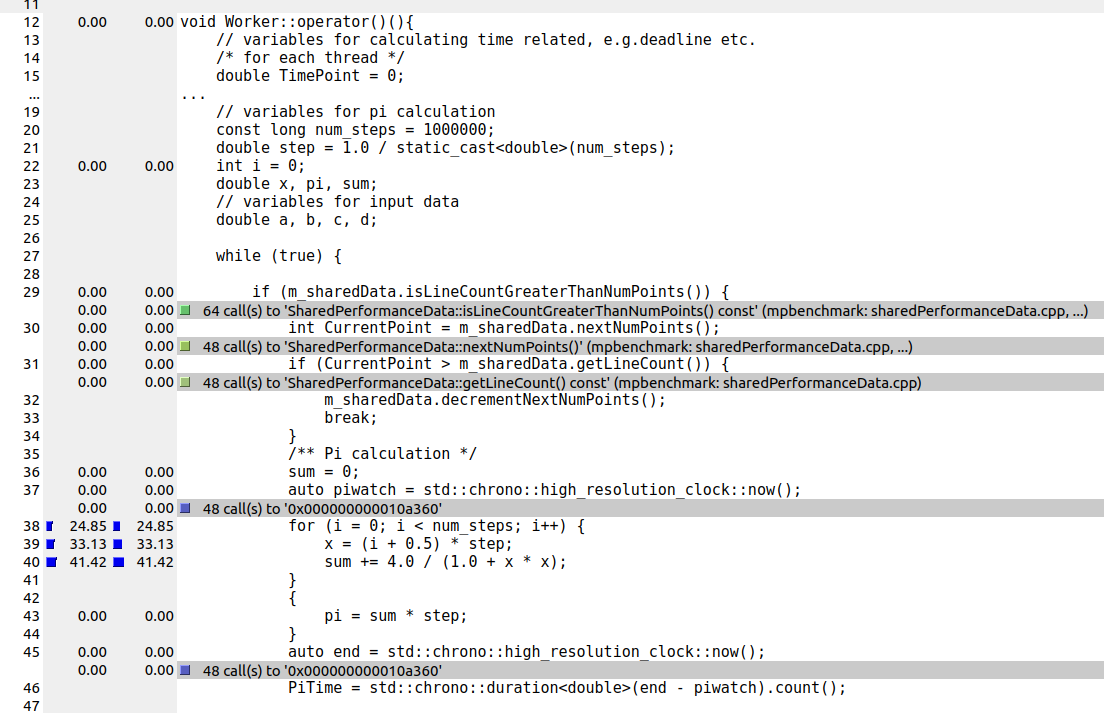
\includegraphics[width=1\textwidth, height=20cm]{~/Documents/Part_D_Modules/Individual_Project/Individual_report/figures/valgrind_mpbenchmark.png} % Adjust the path and width as needed
	\caption{\texttt{Calgrind} profiling results on the \texttt{mpbenchmark} application. Ir - Instruction Fetch, CEst - Cycle estimation.}
	\label{fig:mpbenchmark_profiled} % Use this label to reference the figure
\end{figure} 

Code for implementing the approximation of $\pi$ using single and double point floating precision with \texttt{NEON} instructions are shown in listings ~\ref{lst:neon_float} and ~\ref{lst:neon_double}.

\begin{lstlisting}[
	caption={Approximation of $\pi$ using single point precision \texttt{NEON} instructions.},
	label={lst:neon_float}
	]
double Worker::approximatePi(){
	double pi = 0.0;
	static constexpr long num_steps = 1000000;
	static constexpr double step = 1.0 / static_cast<double>(num_steps);
	
	#if defined(__AVX2__)
	// Insert AVX2 specific code here ...

	#elif defined(__ARM_NEON)
	// Insert NEON specific code here
	float32_t f_step = 1.0f / static_cast<float32_t>(num_steps); // Using float for NEON
	float32x4_t vec_step = vdupq_n_f32(f_step);
	float32x4_t vec_half_step = vdupq_n_f32(0.5f * f_step);
	float32x4_t vec_one = vdupq_n_f32(1.0f);
	float32x4_t vec_four = vdupq_n_f32(4.0f);
	float32_t sum = 0.0f; // Using float for NEON
	
	for (int i = 0; i < num_steps; i += 4) {
		float32x4_t vec_i = vsetq_lane_f32(i + 3, vsetq_lane_f32(i + 2, vsetq_lane_f32(i + 1, vsetq_lane_f32(i, vdupq_n_f32(0.0f), 0), 1), 2), 3);
		float32x4_t vec_x = vaddq_f32(vmulq_f32(vec_i, vec_step), vec_half_step);
		float32x4_t vec_temp = vdivq_f32(vec_four, vaddq_f32(vec_one, vmulq_f32(vec_x, vec_x)));
		sum += vaddvq_f32(vec_temp); // Horizontal sum of vector elements
	}
	
	pi = sum * f_step;
	#else
	// Insert regular code here ...
	#endif
	return pi;
}
\end{lstlisting}


\begin{lstlisting}[
	caption={Approximation of $\pi$ using double point precision \texttt{NEON} instructions.},
	label={lst:neon_double}
	]
	double Worker::approximatePi(){
		double pi = 0.0;
		static constexpr long num_steps = 1000000;
		static constexpr double step = 1.0 / static_cast<double>(num_steps);
		
		#if defined(__AVX2__)
		// Insert AVX2 specific code here ...
		
		#elif defined(__ARM_NEON)
		// Insert NEON specific code here
		float64x2_t vec_step = vdupq_n_f64(step);
		float64x2_t vec_half_step = vdupq_n_f64(0.5 * step);
		float64x2_t vec_one = vdupq_n_f64(1.0);
		float64x2_t vec_four = vdupq_n_f64(4.0);
		float64_t sum = 0.0;
		
		for (int i = 0; i < num_steps; i += 2) {
			// Since direct lane setting for float64x2_t via intrinsics like vsetq_lane_f64 isn't straightforward,
			// We compute x and its index scalarly and then load them into vectors.
			double x0 = (i + 0.5) * step;
			double x1 = (i + 1.5) * step;
			float64x2_t vec_x = {x0, x1}; // Directly initialize the vector with double values.
			
			float64x2_t vec_temp = vdivq_f64(vec_four, vaddq_f64(vec_one, vmulq_f64(vec_x, vec_x)));
			sum += vaddvq_f64(vec_temp); // Horizontal sum of vector elements.
		}
		
		pi = sum * step;
		#else
		// Insert regular code here ...
		#endif
		return pi;
	}
\end{lstlisting}

To use \texttt{AVX2} instructions for the application, the following changes were made to the \texttt{CMakeLists.txt} file, however no changes were required to use \texttt{NEON} instructions, see listing ~\ref{lst:cmake_simd}.

\begin{lstlisting}[
	language=bash,
	caption={Adding \texttt{-mavx2 -mfma} flags to the \texttt{CMake} file to allow the project to use \texttt{AVX2} instructions.},
	label={lst:cmake_simd}
	]
	# Compiler optimizations
	include(CheckCXXCompilerFlag)
	
	# Check and enable AVX2 and FMA for x86_64 architecture
	CHECK_CXX_COMPILER_FLAG("-mavx2" COMPILER_SUPPORTS_AVX2)
	CHECK_CXX_COMPILER_FLAG("-mfma" COMPILER_SUPPORTS_FMA)
	if (COMPILER_SUPPORTS_AVX2 AND COMPILER_SUPPORTS_FMA)
	target_compile_options(${PROJECT_NAME} PRIVATE -mavx2 -mfma)
	endif()
	
	if (CMAKE_SYSTEM_PROCESSOR MATCHES "arm" OR CMAKE_SYSTEM_PROCESSOR MATCHES "aarch64")
	# For ARMv8-A (aarch64), NEON is always available. No need for -mfpu=neon
	# We can set architecture-specific flags if necessary, but for NEON, it's not required.
	endif
\end{lstlisting}

Results collected from Raspberry Pi 4 can be seen in figures ~\ref{fig:mpbenchmark_rpi4_plot} and ~\ref{fig:mpbenchmark_rpi4_speedup_plot}. 

\begin{figure}[H] % Positioning preference: here, top, bottom, page
	\centering
	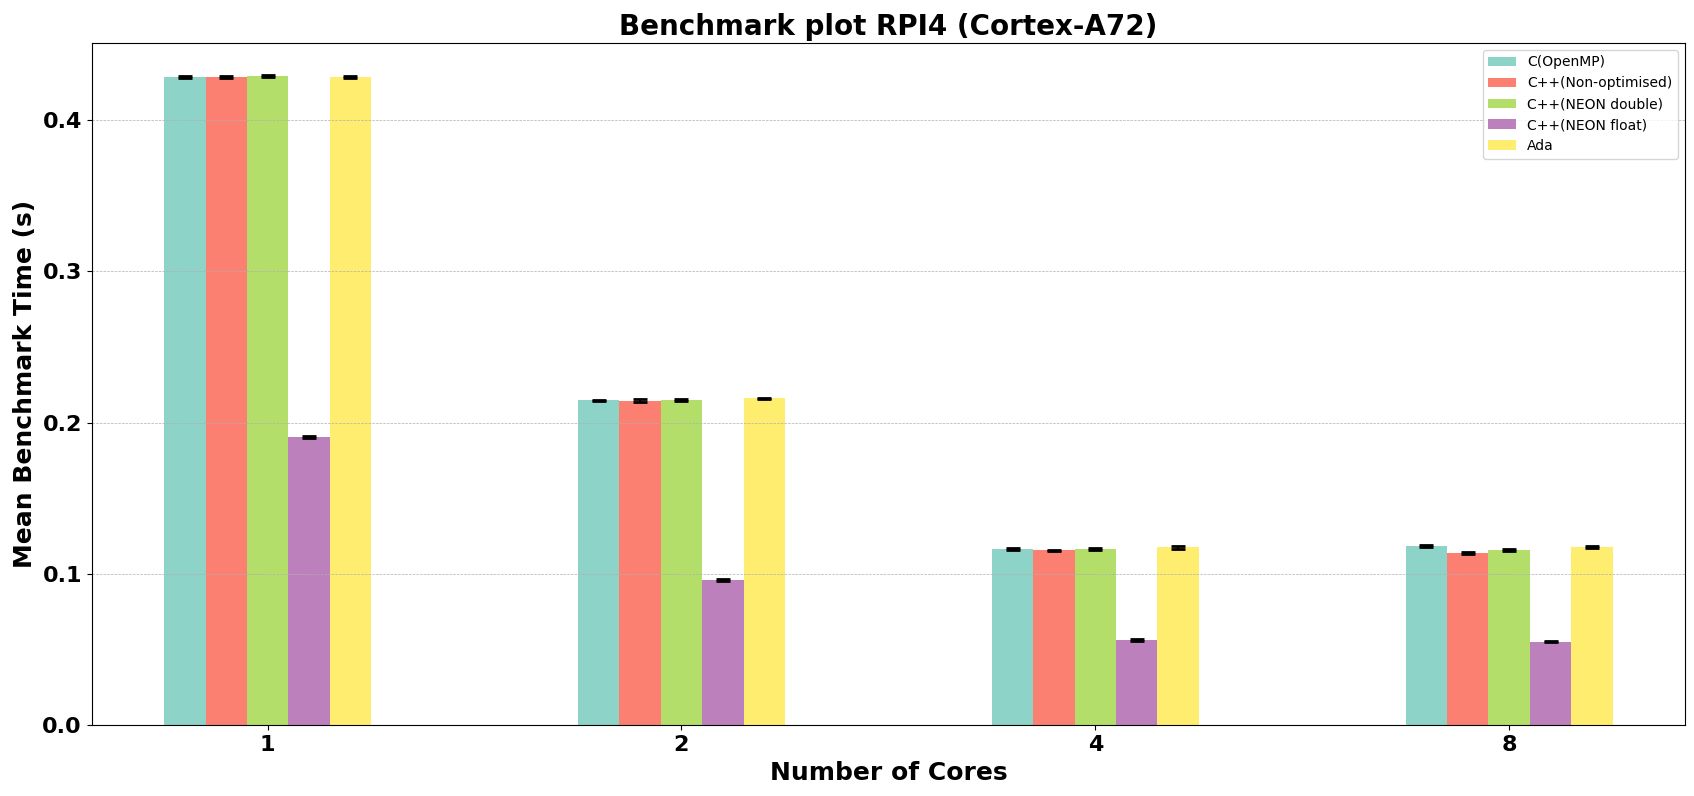
\includegraphics[width=1\textwidth, height=20cm]{~/Documents/Part_D_Modules/Individual_Project/Individual_report/figures/mpbenchmark_rpi4.png} % Adjust the path and width as needed
	\caption{Mean benchmark plot of results collected from Raspberry Pi 4(in seconds). The error bars represent 95\% confidence interval. (Lower is better).}
	\label{fig:mpbenchmark_rpi4_plot} % Use this label to reference the figure
\end{figure}

\begin{figure}[H] % Positioning preference: here, top, bottom, page
	\centering
	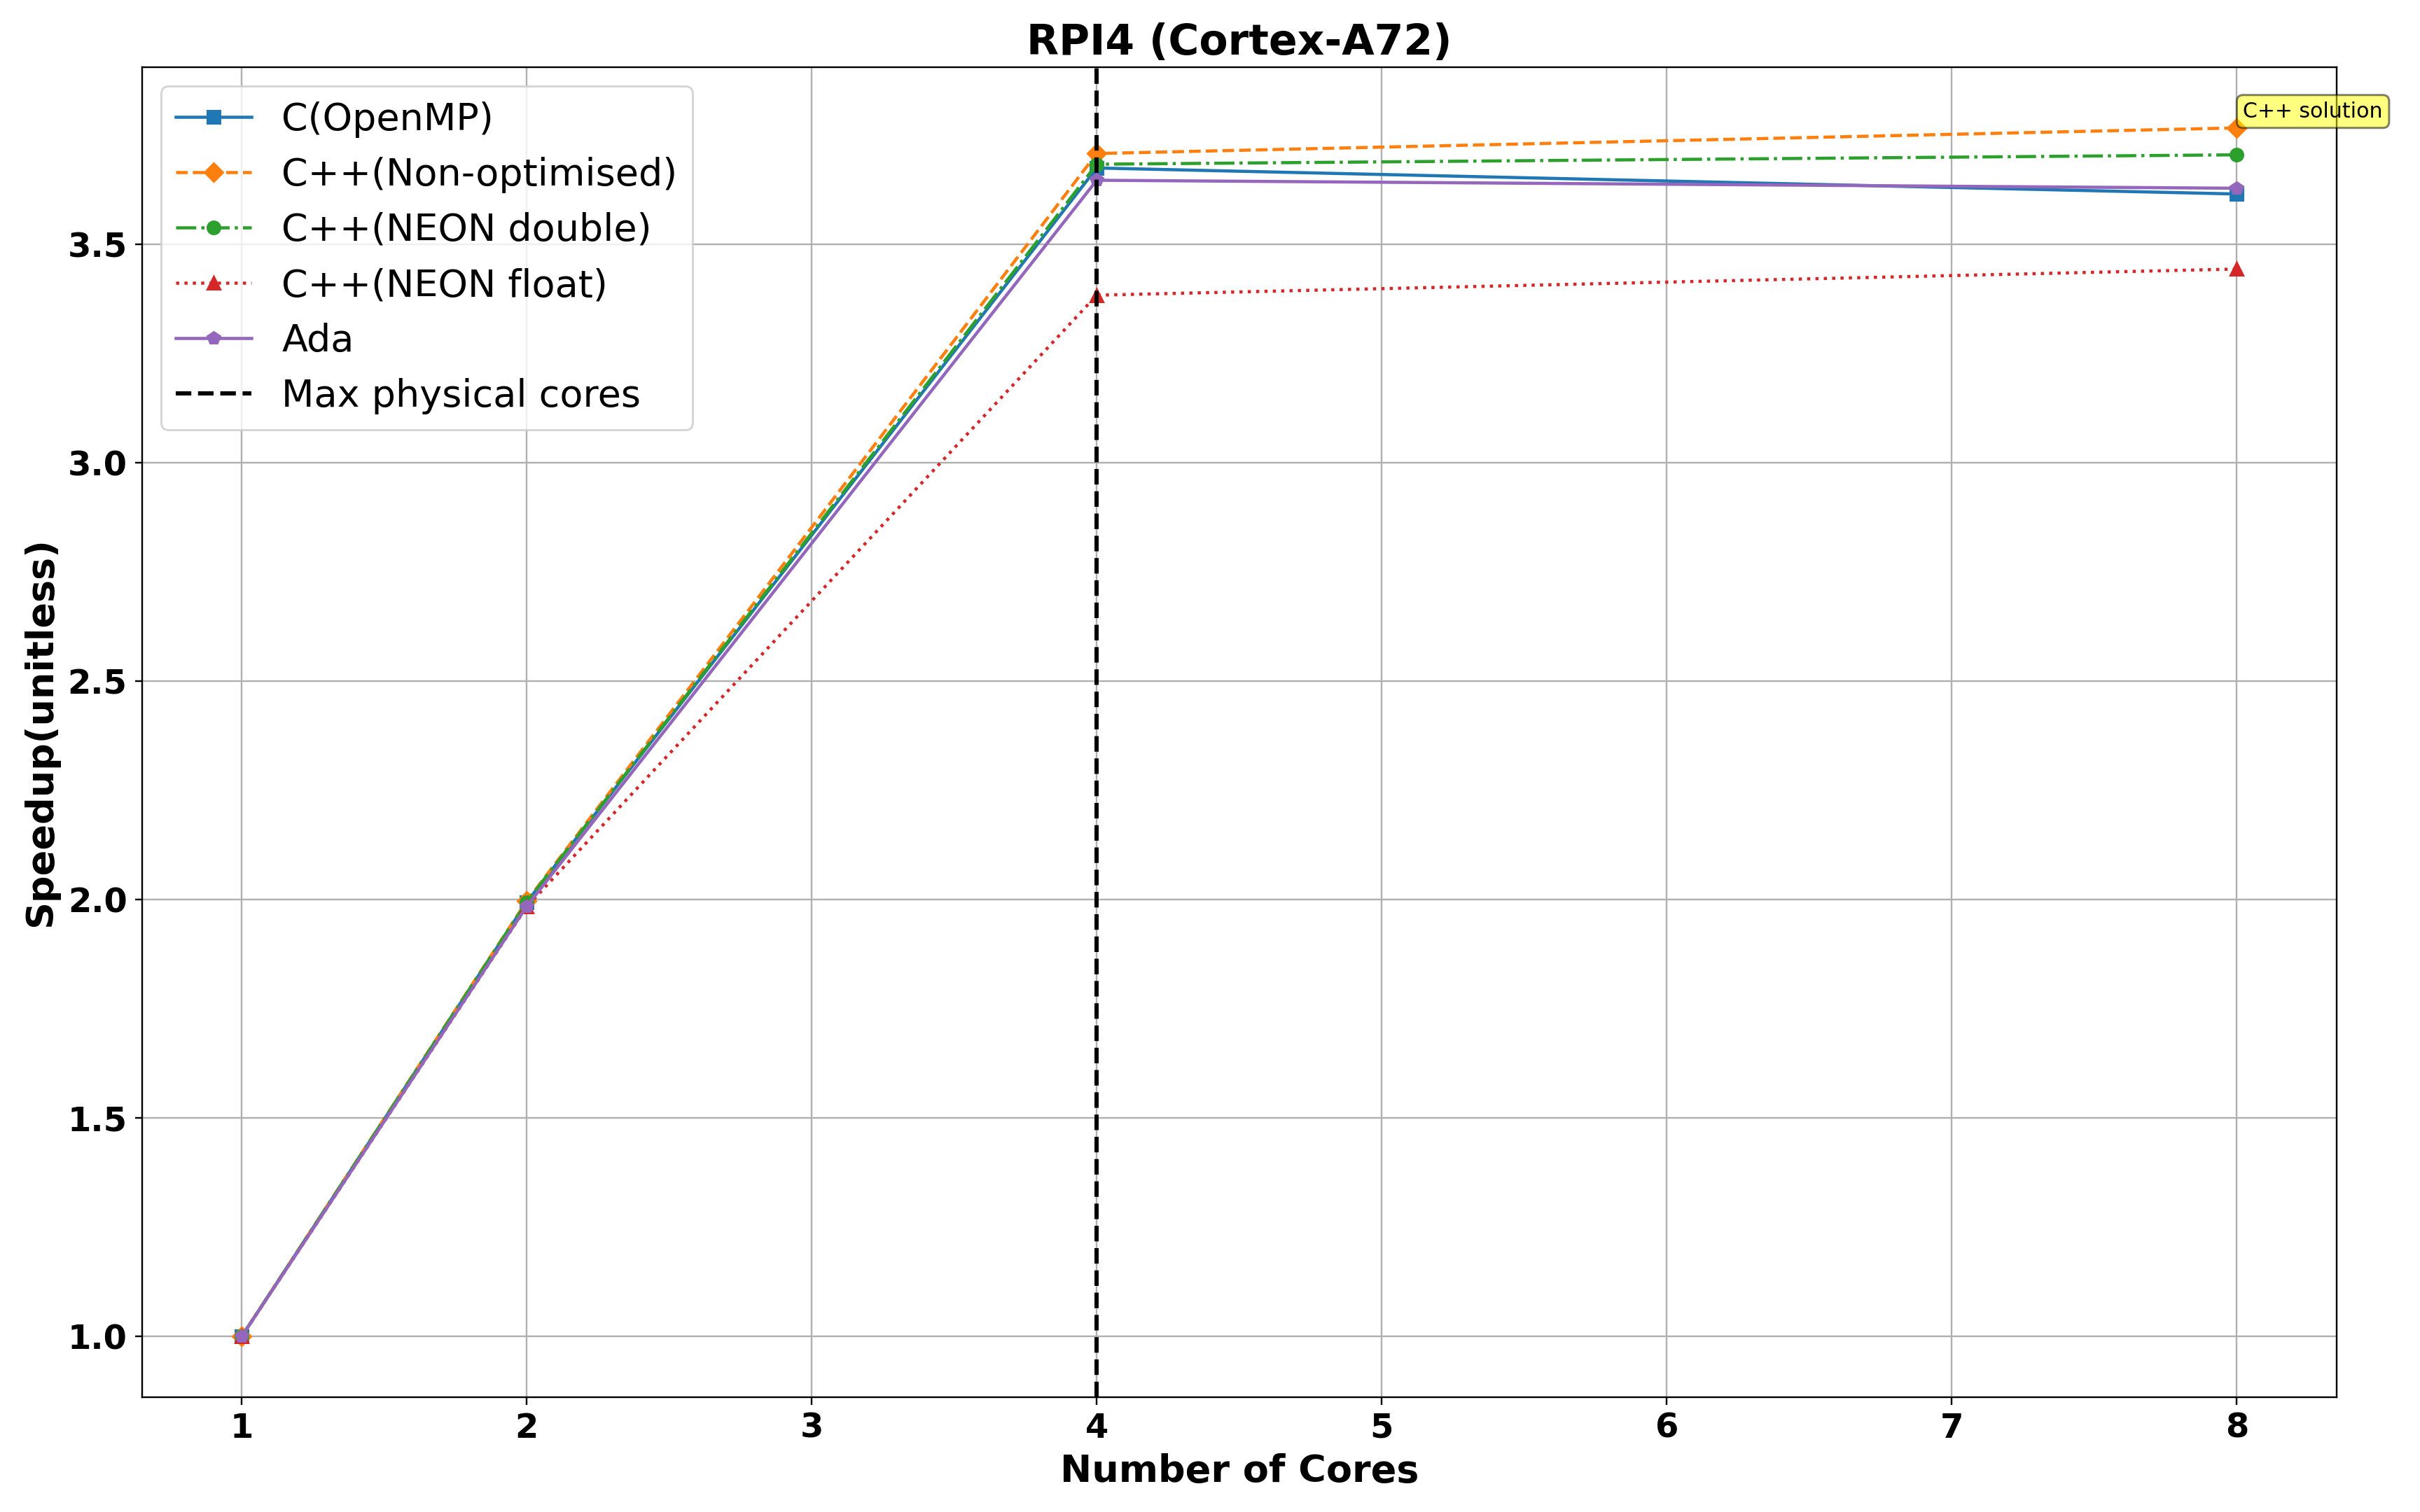
\includegraphics[width=1\textwidth, height=20cm]{~/Documents/Part_D_Modules/Individual_Project/Individual_report/figures/mpbenchmark_rpi4_speedup.png} % Adjust the path and width as needed
	\caption{Speedup plot collected from Raspberry Pi 4 processor. The vertical black line shows the maximum physical cores of the processor. (Higher is better).}
	\label{fig:mpbenchmark_rpi4_speedup_plot} % Use this label to reference the figure
\end{figure}

\section{Objective 2: \texttt{MobileNet}}

The \texttt{MobileNet} repository\cite{mobilenet_repo} contained some outdated portions of the code which were updated, certain parts of the code contained Chinese language which were translated into English and \texttt{CMake} build software was used to setup the \texttt{MobileNet} application. 

The main updates required to the original \texttt{MobileNet} repository\cite{mobilenet_repo} were inside the \texttt{readdata.cpp} file (listing ~\ref{lst:mobilenet_updates}). 

\begin{lstlisting}[
	caption={Updating the \texttt{ReadData::ReadInput()} function to use the latest \texttt{OpenCV} functions.},
	label={lst:mobilenet_updates}
	]
float* ReadData::ReadInput(const char* pcName) {
	std::cout << "Reading Picture: " << pcName << "..." << std::endl;
	
	// Use cv::Mat for image representation
	cv::Mat srcImage = cv::imread(pcName, cv::IMREAD_UNCHANGED);
	if (srcImage.empty()) {
		std::cerr << "Error: Image not loaded." << std::endl;
		return nullptr;
	}
	
	// Resize image
	cv::Mat dstImage;
	cv::resize(srcImage, dstImage, cv::Size(m_nInputWidth, m_nInputHeight), 0, 0, cv::INTER_LINEAR);
	
	int nOutputIndex = 0;
	
	for (int i = 0; i < dstImage.rows; i++) {
		for (int j = 0; j < dstImage.cols; j++) {
			nOutputIndex = i * m_nInputWidth + j;
			cv::Vec3b pixel = dstImage.at<cv::Vec3b>(i, j);
			m_pfInputData[nOutputIndex] = static_cast<float>(pixel[0]) - m_pfMean[nOutputIndex];
			m_pfInputData[nOutputIndex + m_nImageSize] = static_cast<float>(pixel[1]) - m_pfMean[nOutputIndex + m_nImageSize];
			m_pfInputData[nOutputIndex + 2 * m_nImageSize] = static_cast<float>(pixel[2]) - m_pfMean[nOutputIndex + 2 * m_nImageSize];
		}
	}
	
	std::cout << "Reading Picture Done..." << std::endl;
	
	return m_pfInputData;
}
\end{lstlisting}

The application was modified to have three command line arguments, this served primarily to make testing and collecting benchmark results easier for development purposes. The three arguments are as follows and can be seen in code in listing ~\ref{lst:mobilenet_command_line_arguments}:

\begin{enumerate}
	\item \texttt{test\_all}: This argument can be altered to either test one image or test all images in the data folder.  
	\item \texttt{write\_to\_file}: This argument is for writing benchmark data to a \texttt{.txt} file, this was useful for development purposes. It is recommended to leave this blank, so the project does not save any benchmark data. 
	\item \texttt{threads}: The number of threads that will be used by the application. It can be left blank to use the maximum number of available threads.  
\end{enumerate}

\begin{lstlisting}[
	caption={Altering the \texttt{MobileNet} application to use three command line arguments. \texttt{./mobilenet [test\_all] [write\_to\_file] [threads]}},
	label={lst:mobilenet_command_line_arguments}
	]
	int main(int argc, char* argv[])
	{
		//---------------------------Command line app logic
		bool testAllImages = false;
		bool writeDataToFile = false;  // Declare the variable to handle write to file logic
		bool g_DebugMode = true;       // Default debug mode setting
		int numThreads = 1;            // Default to 1 thread unless specified
		
		if (argc > 1) {
			std::string firstArg(argv[1]);
			testAllImages = (firstArg == "test_all");
		}
		if (argc > 2) {
			std::string secondArg(argv[2]);
			writeDataToFile = (secondArg == "write_to_file");
			g_DebugMode = !writeDataToFile; 
		}
		if (argc > 3) {
			numThreads = std::atoi(argv[3]);
			if (numThreads <= 0) {
				numThreads = omp_get_max_threads();  // Ensure OpenMP is included if used
			}
		}
		//--------------------------------------------------
		// Further logic and operations can follow here
	}
\end{lstlisting}


\texttt{Calgrind} profiling results from the \texttt{MobileNet} application show the following functions with the highest self-cost, these were \texttt{ConvLayer::forward}, \texttt{BatchNormalLayer::forward} and \texttt{ConvLayer::Addpad} as seen in figure ~\ref{fig:mobilenet_profiling}.

\begin{figure}[H] % Positioning preference: here, top, bottom, page
	\centering
	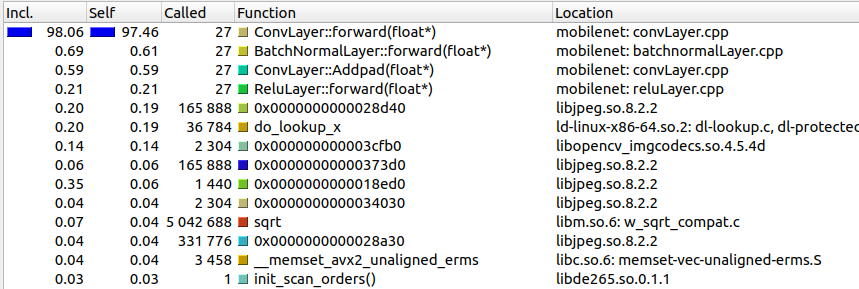
\includegraphics[width=1\textwidth, height=20cm]{~/Documents/Part_D_Modules/Individual_Project/Individual_report/figures/mobilenet_profiling.png} % Adjust the path and width as needed
	\caption{\texttt{Calgrind} profiling results, functions with the highest self-cost.}
	\label{fig:mobilenet_profiling} % Use this label to reference the figure
\end{figure}


The parallelisation of functions \texttt{BatchNormalLayer::forward} and \texttt{ConvLayer::Addpad} can be found in listings ~\ref{lst:mobilenet_function1_parallel} and ~\ref{lst:mobilenet_function2_parallel}.

\begin{lstlisting}[
	caption={Parallelising the \texttt{BatchNormalLayer::forward()} function.},
	label={lst:mobilenet_function1_parallel}
	]
void BatchNormalLayer::forward(float *pfInput) 
{
	#pragma omp parallel for collapse(2) shared(m_nInputNum, m_nInputSize, pfInput, m_pfOutput, m_pfFiller, m_pfMean, m_pfVar, m_pfBias) 
	for (int i = 0; i < m_nInputNum; i++)
	{
		for (int j = 0; j < m_nInputSize; j++)
		{
			int nOutputIndex = i * m_nInputSize + j;
			
			m_pfOutput[nOutputIndex] = m_pfFiller[i] * ((pfInput[nOutputIndex] - m_pfMean[i])
			/ sqrt(m_pfVar[i] + 1e-5)) + m_pfBias[i];
		}
	}
}
\end{lstlisting}


\begin{lstlisting}[
	caption={Parallelising the \texttt{ConvLayer::Addpad()} function If the \texttt{EMBEDDED\_PROC} is not set.},
	label={lst:mobilenet_function2_parallel}
	]
void ConvLayer::Addpad(float *pfInput)
{
	// Only use OpenMP pragmas if EMBEDDED_PROC is not defined, such as on a laptop/desktop CPU 
	#ifndef EMBEDDED_PROC
	#pragma omp parallel for collapse(2)
	#endif
	for (int m = 0; m < m_nInputNum; m++)
	{
		for (int i = 0; i < m_nInputPadWidth; i++)
		{
			for (int j = 0; j < m_nInputPadWidth; j++)
			{
				if ((i < m_nPad) || (i >= m_nInputPadWidth - m_nPad))
				{
					m_pfInputPad[m * m_nInputPadSize + i * m_nInputPadWidth + j] = 0;
				}
				else if ((j < m_nPad) || (j >= m_nInputPadWidth - m_nPad))
				{
					m_pfInputPad[m * m_nInputPadSize + i * m_nInputPadWidth + j] = 0;
				}
				else
				{
					m_pfInputPad[m * m_nInputPadSize + i * m_nInputPadWidth + j] = pfInput[m * m_nInputSize + (i - m_nPad) * m_nInputWidth + (j - m_nPad)];
				}
			}
		}
	}
}
\end{lstlisting}

% Addition of command line arguments
% Valgrind results 
% All the parallelised code

Results collected from Raspberry Pi 4 can be seen in figures ~\ref{fig:mobilenet_rpi4_plot} and ~\ref{fig:mobilenet_rpi4_speedup}. 

\begin{figure}[H] % Positioning preference: here, top, bottom, page
	\centering
	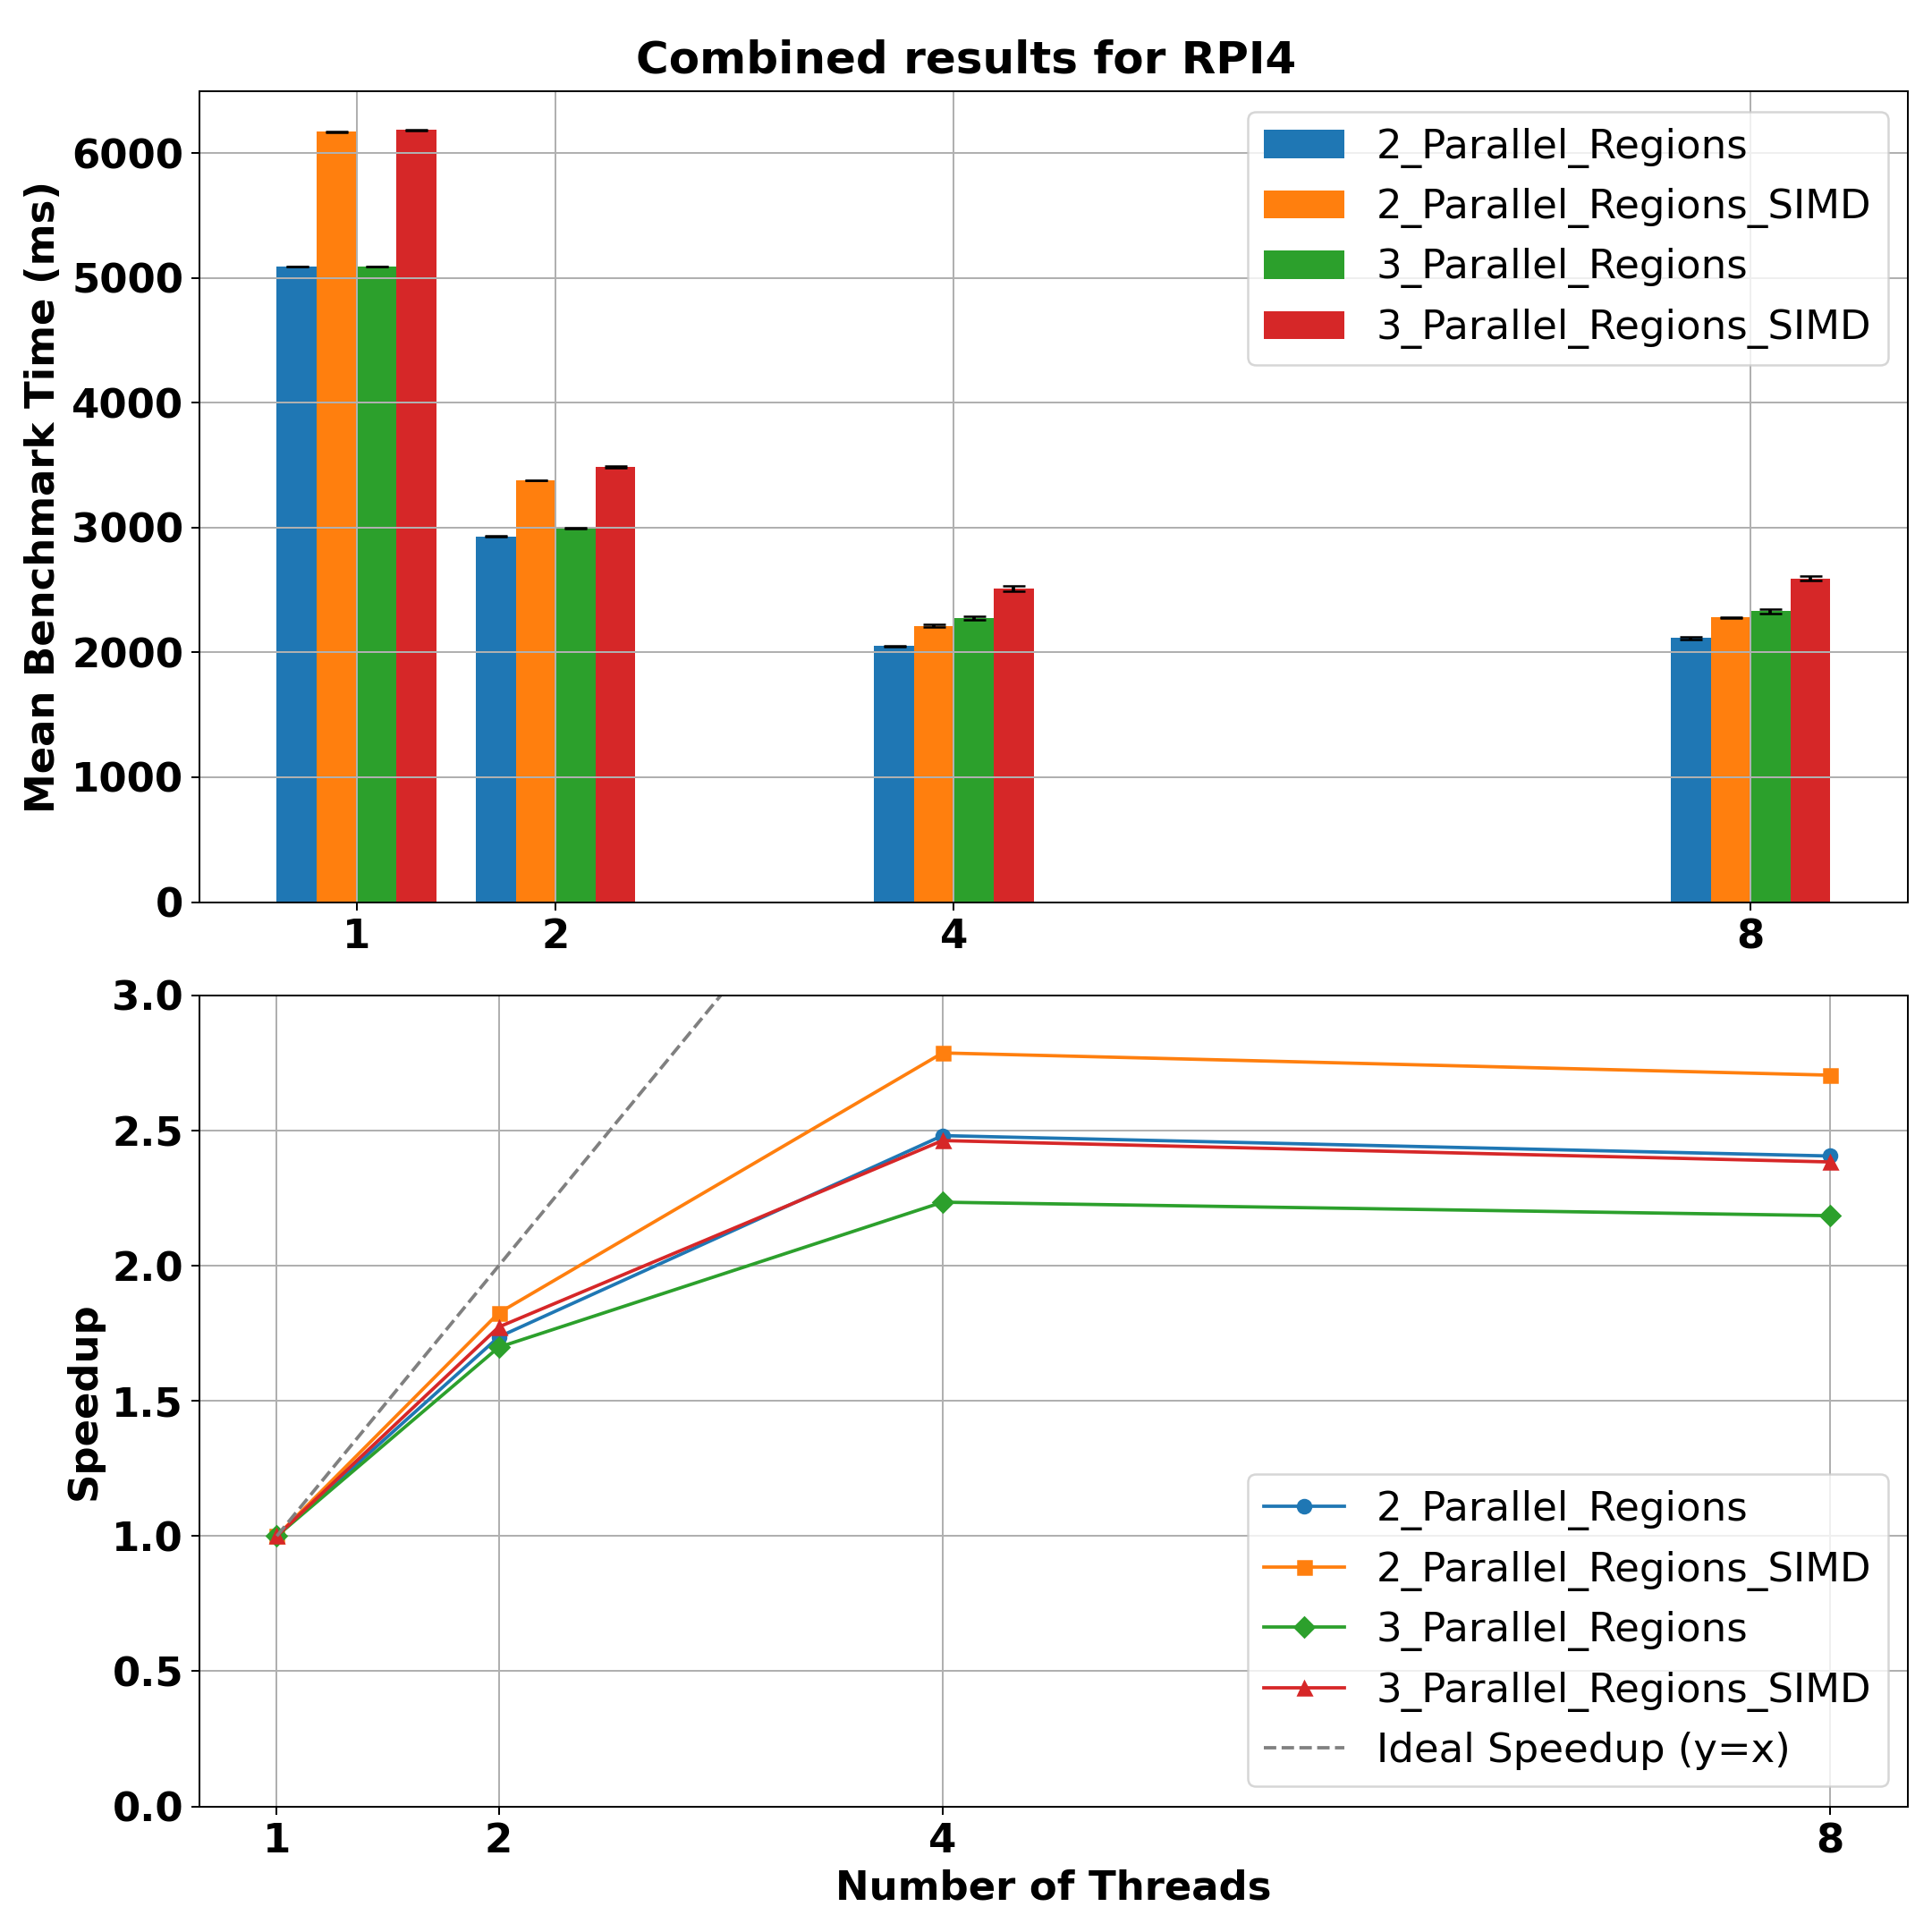
\includegraphics[width=1\textwidth, height=20cm]{~/Documents/Part_D_Modules/Individual_Project/Individual_report/figures/mobilenet_rpi4.png} % Adjust the path and width as needed
	\caption{Mean benchmark plot of results collected from \texttt{Cortex A-72} processor(in milliseconds). (Lower is better).}
	\label{fig:mobilenet_rpi4_plot} % Use this label to reference the figure
\end{figure}

\begin{figure}[H] % Positioning preference: here, top, bottom, page
	\centering
	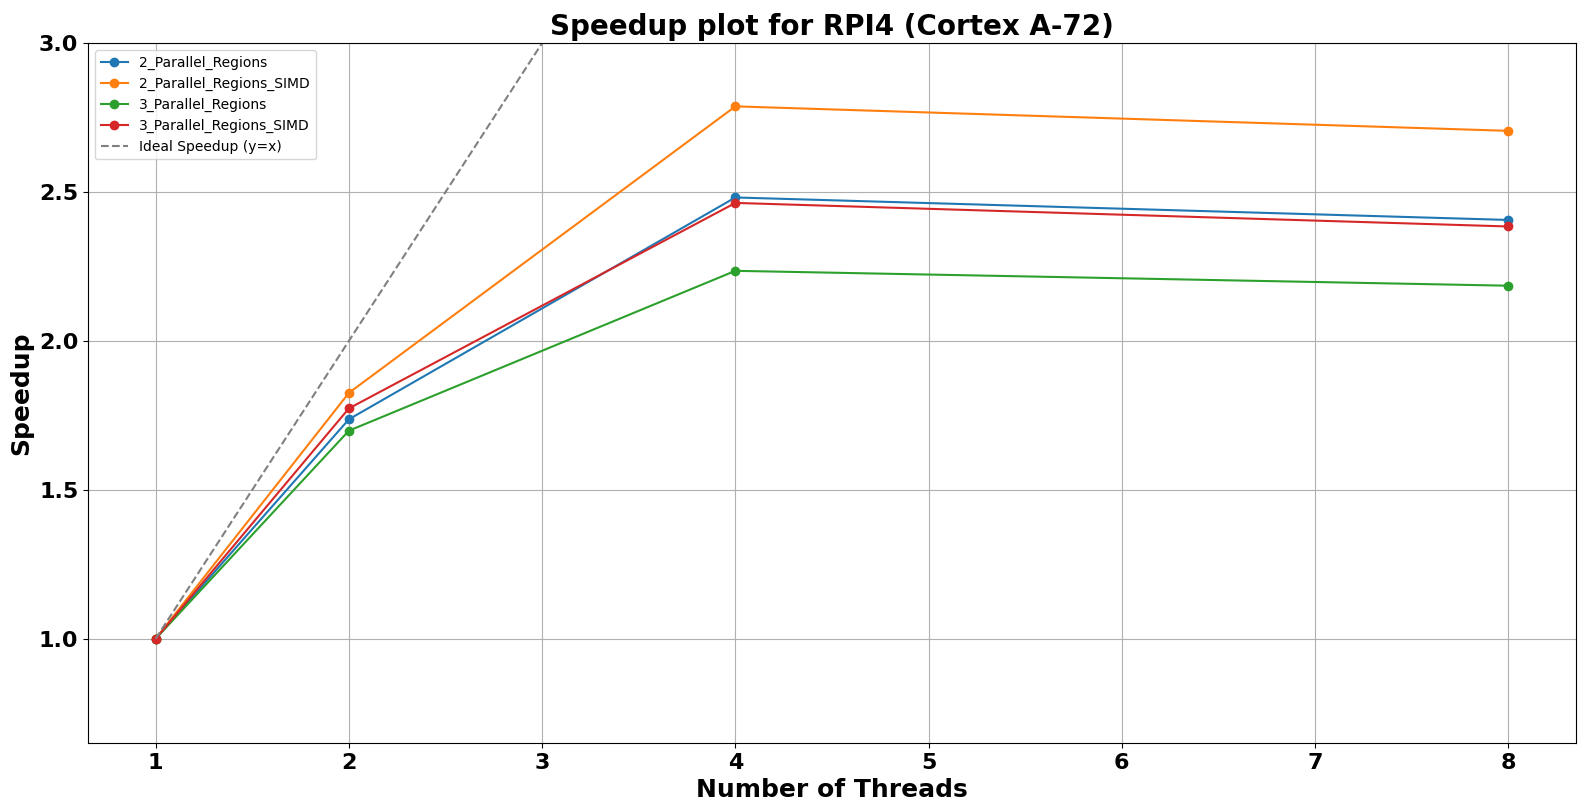
\includegraphics[width=1\textwidth, height=20cm]{~/Documents/Part_D_Modules/Individual_Project/Individual_report/figures/mobilenet_rpi4_speedup.png} % Adjust the path and width as needed
	\caption{Speedup plot comparing different solutions with results collected from \texttt{Cortex A-72} processor. (Higher is better).}
	\label{fig:mobilenet_rpi4_speedup} % Use this label to reference the figure
\end{figure}

\section{Objective 3: \texttt{DeBaTE-FI} platform}
\label{sec:app_obj3}

The application was profiled using \texttt{py-spy} tool. The application spawned multiple processes, therefore they were profiled separately. Profiling results from the process responsible for the GUI of the application are shown in figure ~\ref{fig:debate_profile_1} and the profiling results from the process responsible for communicating with the MCUs are shown in figure ~\ref{fig:debate_profile_2}.

\begin{figure}[H] % Positioning preference: here, top, bottom, page
	\centering
	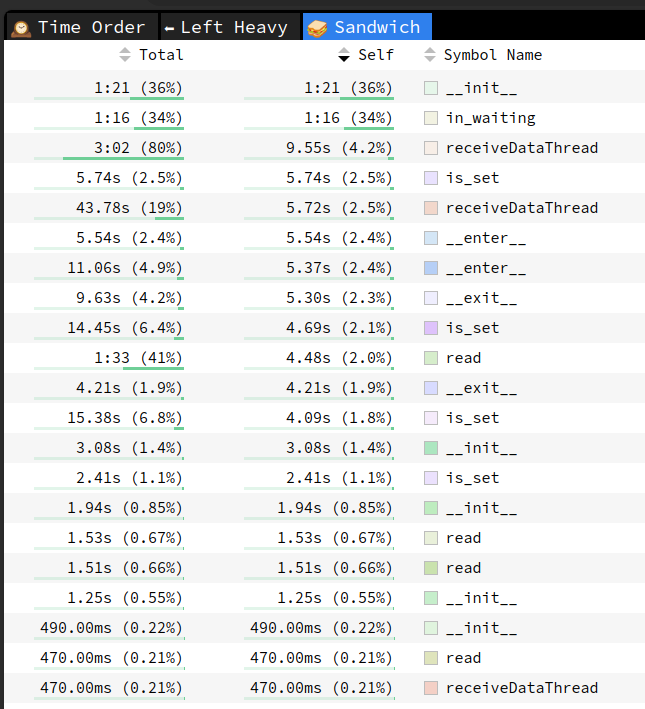
\includegraphics[width=1\textwidth, height=20cm]{~/Documents/Part_D_Modules/Individual_Project/Individual_report/figures/debate_fi_platform_app.png} % Adjust the path and width as needed
	\caption{Profiling results for the application GUI process visualised in \texttt{speedscope} web application\cite{speedscope_app}. }
	\label{fig:debate_profile_1} % Use this label to reference the figure
\end{figure}

\begin{figure}[H] % Positioning preference: here, top, bottom, page
	\centering
	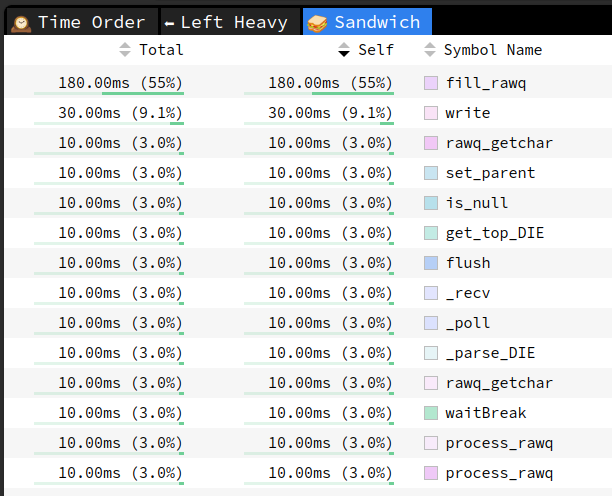
\includegraphics[width=1\textwidth, height=20cm]{~/Documents/Part_D_Modules/Individual_Project/Individual_report/figures/debate_fi_platform_openocd.png} % Adjust the path and width as needed
	\caption{Profiling results for the \texttt{OpenOCD/telnet} process visualised in \texttt{speedscope} web application\cite{speedscope_app}.}
	\label{fig:debate_profile_2} % Use this label to reference the figure
\end{figure}


The \texttt{C++} wrapper was created by emulating the \texttt{Python's} \texttt{telnetlib} library.Using the code in listing ~\ref{lst:open_ocd_class} the following functions require emulation:

\begin{enumerate}
	\item \texttt{read\_some()}
	\item \texttt{write()}
	\item \texttt{Exec()}
	\item \texttt{Readout()}
\end{enumerate}


\begin{lstlisting}[
	caption={Functions used from \texttt{Python's} \texttt{telnetlib} library.},
	label={lst:open_ocd_class}
	]
	
import telnetlib

class OpenOCD:
	def __init__(self, Host="localhost", Port=4444):
		try:
			self.tn = telnetlib.Telnet(Host, Port)
		except ConnectionRefusedError as e:
			print("ERROR: Could not open port",Port)
			raise e
		self.Readout()

#
# Communication functions
#
	def Readout(self):
		s = ''
		Lines = []
		while True:
			s += self.tn.read_some().decode('UTF-8') # 'telnetlib' function called
			l = s.splitlines()
		if len(l) > 1:
			for s in l[:-1]:
				if len(s) > 0:
					Lines.append(s)
			s = l[-1]
	if s == '> ':
		return Lines

	def Exec(self, Cmd, *args):
		Text = Cmd
		for arg in args:
			if arg:
				Text += ' ' + arg
		Text += '\n'
		self.tn.write(bytearray(Text, 'UTF-8')) # 'telnetlib' function called
		return self.Readout()
\end{lstlisting}

Using the open-source \texttt{telnet} libraries in \texttt{C++}: \texttt{telnetpp}\cite{telnetpp_library} and \texttt{serverpp}\cite{serverpp_library} the necessary functions were created in the wrapper class seen in figure ~\ref{fig:telnetlibcpp_UML}. Listing ~\ref{lst:c++_telnetlibcpp} shows the code:

\begin{lstlisting}[
	caption={\texttt{C++} wrapper class to integrate with the \texttt{Python} application. Emulating functions \texttt{read\_some()}, \texttt{write()}, \texttt{Exec()} and \texttt{Readout()}. },
	label={lst:c++_telnetlibcpp}
	]
std::vector<serverpp::byte> TelnetlibCpp::read_some() {
	incoming_data_ = false; // Ensure the flag is reset before starting the async operation
	receivedData_.clear(); // Clear previous data
	// Return a copy of the data or move receivedData as appropriate
	telnet_session_.async_read([this](gsl::span<const serverpp::byte> data) {
		if (!data.empty()) {
			// Directly assign the data since receivedData is a member variable
			receivedData_.assign(data.begin(), data.end());
		}
		incoming_data_ = true; // Indicate that data has been received or the operation is complete
	});
	// Efficiently wait for the async operation to complete using io_context.run_one()
	while (!incoming_data_) {
		io_context_.run_one();
	}
	// Return a copy of the data or move receivedData as appropriate
	return receivedData_;
}

void TelnetlibCpp::write(const std::vector<serverpp::byte>& data) {
	// Assuming 'serverpp::byte' is compatible with 'telnetpp::byte'
	// Wrap the data in a 'telnetpp::bytes' variant to create a 'telnetpp::element'
	telnetpp::bytes byte_data(data.data(), data.size());
	telnetpp::element elem = byte_data;  // Implicitly converts to variant
	
	// Now call the write method with the constructed element
	telnet_session_.write(elem);
}

std::vector<std::string> TelnetlibCpp::Exec(const std::string& cmd, const std::vector<std::string>& args) {
	std::string text = cmd;
	for (const auto& arg : args) {
		if (!arg.empty()) {
			text += ' ' + arg;
		}
	}
	text += '\n';
	
	// write(Cmd), write directly to avoid unnecessary conversions 
	telnetpp::bytes byte_data(reinterpret_cast<const std::uint8_t*>(text.data()), text.size());
	telnetpp::element elem = byte_data;
	telnet_session_.write(elem); 
	//-----------------------------------------------------------------------------------------
	
	// Read and return the output
	return Readout();
}

std::vector<std::string> TelnetlibCpp::Readout() {
	std::string s;
	std::vector<std::string> lines;
	
	while (true) {
		std::vector<std::uint8_t> byte_data = read_some();
		std::string chunk(byte_data.begin(), byte_data.end());
		
		s += chunk;
		
		size_t start_pos = 0;
		size_t pos;
		while ((pos = s.find('\n', start_pos)) != std::string::npos) {
			if (pos > start_pos) { // Ignore empty lines
				std::string line(s.begin() + start_pos, s.begin() + pos);
				line.erase(std::remove(line.begin(), line.end(), '\r'), line.end());
				line.erase(std::remove(line.begin(), line.end(), '\x00'), line.end());
				
				if (line.size())
				lines.push_back(std::move(line)); // Use move semantics to avoid copying
			}
			start_pos = pos + 1;
		}
		s.erase(s.begin(), s.begin() + start_pos); // Only erase the processed part
		
		if (s.find('>') != std::string::npos) {
			return lines; // Assuming lines are already filtered correctly
		}
	}
}

\end{lstlisting}

This was integrated into the \texttt{Python} application using a tool called \texttt{pybind11}. This required creating a \texttt{.cpp} file to allow the \texttt{C++} funtions to be called from the \texttt{Python} file, this is seen in listing ~\ref{lst:pybind_c++_file}.

\begin{lstlisting}[
	caption={Preparing our \texttt{C++} class \texttt{telnetlibcpp} using \texttt{pybind11} to be used with \texttt{Python}.},
	label={lst:pybind_c++_file}
	]
#include <pybind11/pybind11.h>
#include <pybind11/stl.h> // For automatic conversion of std::vector
#include "telnetlibcpp.hpp" // Include your class definition

namespace py = pybind11;

PYBIND11_MODULE(telnetlibcpp, m) {
	py::class_<TelnetlibCpp>(m, "TelnetlibCpp")
	.def(py::init<const std::string&, serverpp::port_identifier>())
	.def("Readout", &TelnetlibCpp::Readout) // Bind the Readout function
	// Bind the Exec function, using a lambda to handle optional vector<string> args
	.def("Exec", [](TelnetlibCpp& self, const std::string& cmd, const py::list& args) {
		std::vector<std::string> vecArgs;
		for (const auto& arg : args) {
			if (!arg.is_none()) {
				vecArgs.push_back(arg.cast<std::string>());
			} else {
				// Optionally, handle None values differently, e.g., by inserting an empty string
				// vecArgs.push_back("");
			}
		}
		return self.Exec(cmd, vecArgs);
	})
	.def("read_some", &TelnetlibCpp::read_some)
	.def("write", &TelnetlibCpp::write)
	.def("write_raw_sequence", &TelnetlibCpp::write_raw_sequence)
	.def("run", &TelnetlibCpp::run);
}
\end{lstlisting}

The final step was to compile the \texttt{C++} codes into a shared library(\texttt{.so}) file which was then placed in the directory of the \texttt{Python} application where it needed to be used. Listing ~\ref{lst:cmake_so_file} shows hows this shared library file was created. 

\begin{lstlisting}[
	caption={\texttt{CMake} file to produce a shared library(\texttt{.so}) file of our \texttt{C++} class.},
	label={lst:cmake_so_file}
	]
cmake_minimum_required(VERSION 3.14 FATAL_ERROR)
project(telnetlibcpp)

# Set the C++ standard
set(CMAKE_CXX_STANDARD 17)
set(CMAKE_CXX_STANDARD_REQUIRED ON)
set(CMAKE_EXPORT_COMPILE_COMMANDS ON)

# Optimization flag -O3 for Release builds
set(CMAKE_CXX_FLAGS_RELEASE "-O3")

# Include Pybind11
include(FetchContent)
FetchContent_Declare(
pybind11
GIT_REPOSITORY https://github.com/pybind/pybind11.git
GIT_TAG v2.6.1
)
FetchContent_MakeAvailable(pybind11)

# Find required Boost components in one call
find_package(Boost REQUIRED COMPONENTS container locale)
find_package(serverpp REQUIRED)
find_package(telnetpp 3.0.0 REQUIRED)
find_package(gsl-lite REQUIRED)

# Source files including the Pybind11 binding file
set(SOURCE_FILES
src/telnetlibcpp.cpp
src/pybind_module.cpp  # Your Pybind11 binding source file
)

# Compile as a shared library
add_library(telnetlibcpp SHARED ${SOURCE_FILES})

target_include_directories(telnetlibcpp PRIVATE include)

target_link_libraries(telnetlibcpp
PRIVATE
KazDragon::serverpp
KazDragon::telnetpp
Boost::container
Boost::locale
pybind11::module  # Link against Pybind11 module support
)

# Set output library name and ensure it doesn't have the 'lib' prefix
set_target_properties(telnetlibcpp PROPERTIES PREFIX "" OUTPUT_NAME "telnetlibcpp")
\end{lstlisting}


  % Assuming this file contains your appendices.
\end{appendices}


\end{document}



